% SIAM Article Template
\documentclass[onecolumn,final,a4paper,13pt,reqno]{siamart}

% Information that is shared between the article and the supplement
% (title and author information, macros, packages, etc.) goes into
% ex_shared.tex. If there is no supplement, this file can be included
% directly.

% Packages and macros go here
\usepackage{lipsum}
\usepackage{amsfonts}
\usepackage{graphicx}
\usepackage{epstopdf}
\usepackage{algorithmic}
\usepackage{xspace}
\usepackage{enumitem}
\usepackage[font=small]{caption}
\usepackage{subcaption}
\usepackage{pgfplots}
\usepackage{tikz}
\usepackage[top=3cm,bottom=3cm,left=2.5cm,right=2.5cm]{geometry}

% http://tex.stackexchange.com/questions/81834/whats-the-best-way-to-typeset-c-codes-in-latex
\usepackage{listings}
\usepackage{color}

\definecolor{mygreen}{rgb}{0,0.6,0}
\definecolor{mygray}{rgb}{0.5,0.5,0.5}
\definecolor{mymauve}{rgb}{0.58,0,0.82}

% https://en.wikibooks.org/wiki/LaTeX/Source_Code_Listings
\lstset{%
	language=C++,
	backgroundcolor=\color{white},
	basicstyle=\tiny,
	breakatwhitespace=false,
	breaklines=true,
	captionpos=t,
	commentstyle=\color{mygreen},
	deletekeywords={...},
	escapeinside={\%*}{*)},
	extendedchars=true,
	frame=single,
	keepspaces=true,
	keywordstyle=\color{blue},
	language=Octave,
	%otherkeywords={*,...},
	numbers=left,
	numbersep=5pt,
	numberstyle=\tiny\color{mygray},
	rulecolor=\color{black},
	showspaces=false,
	showstringspaces=false,
	showtabs=false,
	stepnumber=1,
	stringstyle=\color{mymauve},
	tabsize=4,
	title=\lstname
}

\lstdefinestyle{customcpp}{
	belowcaptionskip=0pt,
	breaklines=true,
	%frame=L,
	%xleftmargin=\parindent,
	language=C++,
	showstringspaces=false,
	basicstyle=\scriptsize\ttfamily,
	keywordstyle=\bfseries\color{green!40!black},
	commentstyle=\itshape\color{purple!40!black},
	identifierstyle=\color{blue},
	stringstyle=\color{orange},
}

\lstset{escapechar=@,style=customcpp}

% http://tex.stackexchange.com/questions/8092/placing-equation-number-on-left-with-reqno-option-in-amsart-document-class
\usepackage{environ}
\makeatletter
\NewEnviron{Lalign}{\tagsleft@true\begin{align}\BODY\end{align}}
\makeatother

% http://tex.stackexchange.com/questions/36278/box-around-theorem-statement
% http://tex.stackexchange.com/questions/188051/skipbelow-does-not-work-for-combination-of-mdframed-and-thmtools
%\usepackage{amsthm}
\usepackage{thmtools}
\usepackage{mdframed}

\declaretheoremstyle[
	postfoothook={\vskip 0.35cm},
	mdframed={
		skipabove=0.35cm,
		innerbottommargin=0.2cm,
		innertopmargin=0.2cm,
		innerleftmargin=0.2cm,
		innerrightmargin=0.2cm,
	}
]{skips}

\declaretheorem[style=skips,name={Theorem}]{theoremmd}
\declaretheorem[style=skips,name={Corollary}]{corollarymd}
\declaretheorem[style=skips,name={Lemma}]{lemmamd}
\declaretheorem[style=skips,name={Definition}]{definitionmd}

% http://tex.stackexchange.com/questions/4728/how-do-i-number-equations-only-if-they-are-referred-to-in-the-text
%\usepackage{mathtools}
%\mathtoolsset{showonlyrefs=true}
\usepackage{autonum}

% http://tex.stackexchange.com/questions/5223/command-for-argmin-or-argmax
\DeclareMathOperator*{\argmin}{arg\,min}

% http://tex.stackexchange.com/questions/23773/a-centered-plus-minus-symbol
\newcommand{\rpm}{\raisebox{.2ex}{$\scriptstyle\pm$}}

\ifpdf
  \DeclareGraphicsExtensions{.eps,.pdf,.png,.jpg}
\else
  \DeclareGraphicsExtensions{.eps}
\fi

\makeatletter
\DeclareRobustCommand\onedot{\futurelet\@let@token\@onedot}
\def\@onedot{\ifx\@let@token.\else.\null\fi\xspace}
\def\eg{{e.g}\onedot} \def\Eg{{E.g}\onedot}
\def\ie{{i.e}\onedot} \def\Ie{{I.e}\onedot}
\def\cf{{c.f}\onedot} \def\Cf{{C.f}\onedot}
\def\etc{{etc}\onedot} \def\vs{{vs}\onedot}
\def\wrt{w.r.t\onedot} \def\dof{d.o.f\onedot}
\def\etal{{et al}\onedot}

% proximal map operator
\DeclareRobustCommand{\prox}[1]{%
    \ifmmode
        \text{prox}_{#1}
    \else
        $\text{prox}_{#1}$
    \fi
}
\def\dom{\text{dom}}
\def\per{\text{per}}

% Declare title and authors, without \thanks
\newcommand{\TheTitle}{iPiano: Inertial Proximal Algorithm for Non-Convex Optimization} 
\newcommand{\TheAuthors}{D. Stutz}

% Sets running headers as well as PDF title and authors
\headers{\TheTitle}{\TheAuthors}

% Title. If the supplement option is on, then "Supplementary Material"
% is automatically inserted before the title.
\title{{\TheTitle}}

% Authors: full names plus addresses.
\author{
  David Stutz\thanks{Submitted as part of the seminar "Ausgew\"ahlte Themen der Bildverarbeitung'', WS 2015/2016, and advised by Prof. Berkels, AICES, RWTH Aachen University.}
}

\usepackage{amsopn}
\DeclareMathOperator{\diag}{diag}

% Optional PDF information
\ifpdf
\hypersetup{
  pdftitle={\TheTitle},
  pdfauthor={\TheAuthors}
}
\fi

\begin{document}

\maketitle

% http://tex.stackexchange.com/questions/133144/how-to-change-the-font-size-of-the-whole-abstract-in-the-article-class
\begin{abstract}
	This paper studies the minimization of non-convex and non-smooth composite functions. In particular, we discuss the algorithm proposed by Ochs \etal in \cite{OchsChenBroxPock:2013}, called iPiano. Following \cite{OchsChenBroxPock:2013}, we present a global convergence result for functions satisfying the Kurdyka-Lojasiewicz property \cite{Lojasiewicz:1993,Kurdyka:1998} which is based on the work by Attouch \etal~\cite{AttouchBolteSvaiter:2013}. Furthermore, we discuss the implementation of iPiano and apply the algorithm to image denoising and image segmentation. In contrast to \cite{OchsChenBroxPock:2013}, we use simple denoising functionals instead of Fields of Expert \cite{RothBlack:2009,ChenPockRanftlBischof:2013} to demonstrate that simple functionals may benefit from non-smooth and non-convex terms. Finally, we demonstrate the applicability of the algorithm to image segmentation based on a 2-phase field approximation of the Mumford-Shah functional \cite{Shen:2005}.
\end{abstract}

\section{Introduction}

% TODO introduce common functionals in the required form and motivate algorithm by l1 norm
% TODO references for this stuff
Many image processing and computer vision problems involve complex, possibly non-smooth and/or non-convex optimization problems. Solving these optimization problems efficiently is as important as attaining globally optimal solutions. On the one hand, this requires efficient algorithms and implementations, while on the other hand proving global convergence may require rather involved mathematics and stricter assumptions on the objective to be optimized. In the simplest case, \ie involving a convex and smooth objective, gradient-based approaches and proximal algorithms offer global convergence, see \cite{BoydVandenberghe:2004} and \cite{ParikhBoyd:2014} for details. Proximal algorithms are also applicable to non-smooth objectives, however, computing the proximal map may not necessary be trivial. More recently, splitting algorithms for non-smooth composite objectives have been studied, see \cite{CombettesPesquet:2011}. For non-convex objectives, establishing global convergence is -- in general -- much harder. Recent efforts focussed on objectives satisfying the Kurdyika-Lojasiewicz property \cite{Lojasiewicz:1993,Kurdyka:1998} for which certain algorithms have been shown to converge \cite{AttouchBolteSvaiter:2013}. In this paper, we study the algorithm proposed by Ochs \etal \cite{OchsChenBroxPock:2013} named iPiano meant for non-smooth and non-convex composite functions of the form introduced in Section \ref{subsec:problem}.

\subsection{Outline} We first present the general problem statement and the necessary mathematical background in Sections \ref{subsec:problem} and \ref{subsec:preliminaries}, respectively. Subsequently we briefly discuss relevant related work in Section \ref{sec:related-work}. In the main part, Section \ref{sec:ipiano}, we present the iPiano algorithm and several variants, present convergence analysis and discuss convergence rate as well as implementation details. Finally, in Section \ref{sec:applications}, we discuss applications before concluding in Section \ref{sec:conclusion}.

\subsection{Problem Statement}
\label{subsec:problem}

In this paper we focus on so-called composite functions (also called $C^1$-perturbations of convex functions) of the form
\begin{align}
	\min_{x \in \mathbb{R}^n} h(x) = \min_{x \in \mathbb{R}^n} (f(x) + g(x))\label{eq:problem}
\end{align}
where $f : \mathbb{R}^n \rightarrow \mathbb{R}$ is required to be in $C^1$ but might be non-convex, while $g : \mathbb{R}^n \rightarrow \mathbb{R} \cup \{\infty\}$ is required to be convex but might be non-smooth. We further require $f$ to have $L$-Lipschitz continuous gradient $\nabla f$. For the minimization problem in Equation \eqref{eq:problem} to be well-posed, we require $h$ to be bounded below by some value
\begin{align}
	-\infty < h_{\min} := \inf _{x \in \mathbb{R}^n} h(x)
\end{align}
Furthermore, $h$ is assumed to be coercive, \ie $h(x) \rightarrow \infty$ for $\|x\|_2 \rightarrow \infty$. With $\dom(g) := \{x \in \mathbb{R}^n | g(x) < \infty\}$ being the effective domain of $g$ and $\dom(g) \subset \dom(f)$, it follows that $\dom(h) = \dom(g)$ has to be convex.

% TODO: proper
\subsection{Preliminaries}
\label{subsec:preliminaries}

Before considering the first-order condition for Equation \eqref{eq:problem} we formally restate the requirement on $h$ to be coercive.

\begin{definitionmd}
	A function $h: \mathbb{R}^n \rightarrow \mathbb{R} \cup \{\infty\}$ is called coercive if there exist constants $p, C > 0$ and $q \geq 0$ such that
	\begin{align}
		h(x) \geq C \|x\|_2^p - q\quad \forall x \in \dom(h).
	\end{align}
\end{definitionmd}

Considering the minimization problem in Equation \eqref{eq:problem}, the first-order condition for $x^\ast \in \mathbb{R}^n$ to be a critical point of $h$ is
\begin{align}
	0 \in \partial h(x^\ast) \Leftrightarrow 0 \in \nabla f(x^\ast) + \partial g(x^\ast) \Leftrightarrow - \nabla f(x^\ast) \in \partial g(x^\ast)
\end{align}
where $\nabla f(x^\ast) + \partial g(x^\ast) := \{ \nabla f(x^\ast) + y | y \in \partial g(x^\ast)\}$ and $\partial g(x^\ast) \subset (\mathbb{R}^n)' = \mathbb{R}^n$ is the subdifferential of $g$ at position $x^\ast$ (note that $(\mathbb{R}^n)'$ refers to the dual space of $\mathbb{R}^n$). In the following, we consider $g$ to be proper, closed and convex:

\begin{definitionmd}
	The function $g :\mathbb{R}^n \rightarrow \mathbb{R} \cup \{\infty\}$ is
	\setlist[enumerate,1]{leftmargin=1.25cm}
	\begin{enumerate}[label=(\alph*)]
		\item convex if
	\end{enumerate}
	\begin{align}
		g(tx + (1 - t)\hat{x}) \leq tg(x) + (1- t)g(\hat{x})\quad\forall x,\hat{x} \in \mathbb{R}^n, t \in [0,1];
	\end{align}
	\begin{enumerate}[label=(\alph*)]
		\setcounter{enumi}{1}
		\item proper if $\dom(g) \neq \emptyset$;
		\item and closed if $\text{graph}(g) := \{(x, \xi) \in \mathbb{R}^n \times \mathbb{R} | g(x) \leq \xi\}$ is closed.
	\end{enumerate}
\end{definitionmd}
\setlist[enumerate,1]{leftmargin=0cm}

Furthermore, we expect $g$ to be lower semicontinuous, \ie for all $x \in \dom(g)$ it holds
\begin{align}
	\liminf_{x^{(n)} \rightarrow x} g(x^{(n)}) \geq g(x).
\end{align}
The first-order condition then follows directly from the following definition and the subsequent lemmata:

\begin{definitionmd}
	Let $g : \mathbb{R}^n \rightarrow \mathbb{R} \cup \{\infty\}$ be a proper convex and lower semi continuous function. Then, the subdifferential $\partial g(x)$ of $g$ at position $x \in \dom(g)$ is defined as
	\begin{align}
		\partial g(x) := \{w \in \mathbb{R}^n | g(x) + w^T(\hat{x} - x) \leq g(\hat{x}) \forall \hat{x} \in \mathbb{R}^n\}.\label{eq:subdiff}
	\end{align}\label{def:subgradient}
\end{definitionmd}

The above definition requires $g$ to be proper convex and lower semi continuous. In contrast, Ochs \etal originally introduce (following \cite[Def. 8.3]{Rockafellar:1970}) the Fr\'echet subdifferential, \ie
\begin{align}
	\hat{\partial} g(x) := \{w \in \mathbb{R}^n | \liminf\limits_{x^{(n)} \rightarrow x, x^{(n)} \neq x} \frac{g(x^{(n)}) - g(x) - w^T(x^{(n)} - x)}{|x^{(n)} - x|} \geq 0\},
\end{align}
and the limiting subdifferential, \ie
\begin{align}
	\begin{aligned}
		\partial g(x) := &\{w \in \mathbb{R}^n | \exists (x^{(n)})_{n \in \mathbb{N}} \subset  \mathbb{R}^n, (w^{(n)})_{n \in \mathbb{N}} \subset \mathbb{R}^n\\
		&\text{ such that } x^{(n)} \rightarrow x, g(x^{(n)}) \rightarrow g(x), w^{(n)} \rightarrow w \text{ and } w^{(n)} \in \hat{\partial}g(x^{(n)})\}.\label{eq:limiting-subdiff}
	\end{aligned}
\end{align}
However, following \cite[Prop. 8.12]{Rockafellar:1970}, the equivalence of Equations \eqref{eq:subdiff} and \eqref{eq:limiting-subdiff} follows if $g$ is proper convex.

Following \cite[Thm. 8.6]{Rockafellar:1970}, we first present a basic property of the subdifferential and subsequently establish the first-order condition mentioned before:

\begin{lemmamd}
	For $g: \mathbb{R}^n \rightarrow \mathbb{R} \cup \{\infty\}$ convex and $x \in \mathbb{R}^n$ with $g(x) < \infty$, the set $\partial g(x)$ is closed.\label{lemma:closure}
\end{lemmamd}
\vskip -1em
\begin{lemmamd}
	Let $h = f + g$ with $f: \mathbb{R}^n \rightarrow \mathbb{R}$ in $C^1$ and $g: \mathbb{R}^n \rightarrow \mathbb{R} \cup \{\infty\}$ convex. Then, for $x \in \dom(h)$ it holds
	\begin{align}
		\partial h(x) = \nabla f(x) + \partial g(x).
	\end{align}\label{lemma:dh}
\end{lemmamd}

Now, we have a closer look at $f$; the following lemma proves a useful property of $f$ with $L$-Lipschitz continuous gradient $\nabla f$:

\begin{lemmamd}
	Let $f: \mathbb{R}^n \rightarrow \mathbb{R}$ be in $C^1$ with $L$-Lipschitz continuous gradient $\nabla f$, \ie it exists $L > 0$ is such that
	\begin{align}
		\|\nabla f(x) - \nabla f(\hat{x})\|_2 \leq L\|x - \hat{x}\|_2,\quad\forall x,\hat{x} \in \mathbb{R}^n.
	\end{align}
	Then it holds:
	\begin{align}
		f(x) \leq f(\hat{x}) + \nabla f(\hat{x})^T(x - \hat{x}) + \frac{L}{2}\|x - \hat{x}\|_2^2,\quad\forall x,\hat{x} \in \mathbb{R}^n.\label{eq:descent-lemma}
	\end{align}\label{lemma:lipschitz}
\end{lemmamd}

Note that Ochs \etal require $f$ to have $L$-Lipschitz continuous gradient $\nabla f$ on $\dom(g)$ only; this implies that Equation \eqref{eq:descent-lemma} holds for all $x, \hat{x} \in \dom(g)$.

Turning to $g$, we first define the proximal mapping $\prox {\alpha g}$, which is the basis of proximal algorithms. We note that further discussion and properties can be found in \cite{ParikhBoyd:2014} and \cite{CombettesPesquet:2011}.

\begin{definitionmd}
	For $\hat{x} \in \mathbb{R}^n$ and $g : \mathbb{R}^n \rightarrow \mathbb{R} \cup \{\infty\}$ being a proper closed convex and lower semicontinuous function, the proximal mapping is defined as
	\begin{align}
		\prox {\alpha g} (\hat{x}) := \argmin_{x \in \mathbb{R}^n} \frac{\|x - \hat{x}\|_2^2}{2} + \alpha g(x) \label{eq:prox}
	\end{align}
	where $\alpha > 0$ is a given parameter.\label{def:prox}
\end{definitionmd}

Note that within the literature, the proximal mapping is often written as
\begin{align}
	(I + \alpha \partial g)^{-1}(\hat{x}) := \prox {\alpha g}(\hat{x})
\end{align}
and called resolvent of the subdifferential. Here, $I$ refers to the identity mapping. The requirements on $g$ stated in Definition \ref{def:prox} are necessary for $\prox{\alpha g}$ to be well-defined, \ie there exist a unique minimizer of Equation \eqref{eq:prox}.
	
\section{Related Work}
\label{sec:related-work}

The work by Ochs \etal combines two different lines of research: splitting algorithms and multistep algorithms. Splitting algorithms originate from the proximal point algorithm. These splitting algorithms usually address problems of the form
\begin{align}
	\min_{x \in \mathbb{R}^n} f_1(x) + \ldots + f_k(x)
\end{align}
for convex functions $f_i : \mathbb{R}^n \rightarrow \mathbb{R} \cup \{\infty\}$ which may not be smooth. Different algorithms have been proposed; we refer to the work by Combettes and Pesquet \cite{CombettesPesquet:2011} providing a thorough overview of the different approaches. Furthermore, they show several useful properties of the proximal mapping as given by Definition \ref{def:prox} including an extensive list of known proximal mappings for a wide range of functions. Ochs \etal partly built upon \cite{AttouchBolteSvaiter:2013} where an abstract convergence theorem for functions satisfying the Kurdyika-Lojasiewicz property is shown (see \cite{Lojasiewicz:1993} and \cite{Kurdyka:1998}). Multistep algorithms were first considered by Polyak \cite{Polyak:1964} and use a so-called inertial force (also called momentum term) to improve convergence. In practice, the inertial force is usually computed as the difference of two preceding iterates. Ochs \etal extend the work by Attouch \etal \cite{AttouchBolteSvaiter:2013} by combining a backward-forward splitting scheme with an inertial force.

\section{iPiano}
\label{sec:ipiano}

Following \cite{OchsChenBroxPock:2013} we present different variants of the proposed algorithm, called iPiano, and discuss convergence for functions satisfying the Kurdyika-Lojasiewicz property (formally introduced later) as well as the corresponding convergence rate.

\subsection{Algorithm}
\label{subsec:ipiano-algorithm}

Essentially, iPiano combines forward-backward splitting as discussed in \cite{CombettesPesquet:2011} with a inertial force (also termed momentum term or multistep term). Given an initial starting point $x^{(0)} \in \mathbb{R}^n$ and setting $x^{(-1)} = x^{(0)}$, iterates are computed as
\begin{align}
	x^{(n + 1)} = {\prox {\alpha_n g}} \left(x^{(n)} - \alpha_n \nabla f(x^{(n)}) + \beta_n (x^{(n)} - x^{(n - 1)})\right)\label{eq:iteration}
\end{align}
for step size parameters $(\alpha_n)_{n \in \mathbb{N}}$ and momentum parameters $(\beta_n)_{n \in \mathbb{N}}$. Obviously, the critical aspect of this generic scheme is choosing these parameters appropriately. In the following we discuss different means of choosing $\alpha_n$ and $\beta_n$.

\subsubsection{ciPiano -- Algorithm \ref{alg:cipiano}}

Of course, both the step size parameter and the momentum parameter can be chosen apriori based on knowledge about $f$. In particular, we need to estimate the global Lipschitz constant $L$ of $\nabla f$ in order to choose $\alpha < \frac{2(1 - \beta)}{L}$.

\begin{algorithm}[h]
	\caption{ciPiano: iPiano with constant stepsize and momentum parameter.}
	\label{alg:cipiano}
	\begin{algorithmic}[1]
		\STATE{choose $\beta \in [0, 1)$}
		\STATE{choose $\alpha < \frac{2(1 - \beta)}{L}$}
		\STATE{choose $x^{(0)}$}
		\STATE{$x^{(-1)} := x^{(0)}$}
		\STATE{// Fixed number of iterations; or $\epsilon$-criterion.}
		\FOR{$n = 0, \ldots$}
			\STATE{$x^{(n + 1)} = {\prox {\alpha g}} \left(x^{(n)} - \alpha \nabla f(x^{(n)}) + \beta (x^{(n)} - x^{(n - 1)})\right)$}
		\ENDFOR
	\end{algorithmic}
\end{algorithm}

\begin{algorithm}[h]
	\caption{nmiPiano: iPiano with backtracking to determine the step size parameter.}
	\label{alg:nmipiano}
	\begin{algorithmic}[1]
		\STATE{choose $\beta \in [0, 1)$}
		\STATE{choose $L_{-1} > 0$}
		\STATE{choose $\eta > 1$}
		\STATE{choose $x^{(0)}$}
		\STATE{$x^{(-1)} := x^{(0)}$}
		\STATE{// Fixed number of iterations; or $\epsilon$-criterion.}
		\FOR{$n = 0, \ldots$}
			\STATE{$L_n := \frac{1}{\eta} L_{n - 1}$ // Initial estimate of $L_n$ is $L_{n - 1}$ or alternatively use \eqref{eq:estimate-L}.}
			\REPEAT
				\STATE{$L_n := \eta L_n$ // Next estimate of $L_n$.}
				\STATE{choose $\alpha_n < \frac{2(1 - \beta)}{L_n}$}
				\STATE{$\tilde{x}^{(n + 1)} = {\prox {\alpha_n g}} \left(x^{(n)} - \alpha_n \nabla f(x^{(n)}) + \beta (x^{(n)} - x^{(n - 1)})\right)$ // Re-estimate $\tilde{x}^{(n + 1)}$.}
			\UNTIL{\eqref{eq:lipschitz-condition} is satisifed for $\tilde{x}^{(n + 1)}$}
			\STATE{//Estimated $L_n$ satisfies Equation \eqref{eq:lipschitz-condition} and $\tilde{x}^{(n + 1)}$ is next iterate:}
			\STATE{$x^{(n + 1)} := \tilde{x}^{(n + 1)}$}
		\ENDFOR
	\end{algorithmic}
\end{algorithm}

% TODO satisfies convergence after not increasing L_n anymore.
\subsubsection{nmiPiano -- Algorithm \ref{alg:nmipiano}}

Estimating $L$ automatically can be accomplished via backtracking: given $x^{(n)}$ and $x^{(n + 1)}$, the estimate of the Lipschitz constant $L_n$ in iteration $n \geq 0$ is required to satisfy
\begin{align}
	f(x^{(n + 1)}) \leq f(x^{(n)}) + \nabla f(x^{(n)})^T (x^{(n + 1)} - x^{(n)}) + \frac{L_n}{2} \|x^{(n + 1)} - x^{(n)}\|_2^2\label{eq:lipschitz-condition}
\end{align}
which follows from Lemma \ref{lemma:lipschitz}. Usually, $x^{(n + 1)}$ is re-estimated (based on $\alpha_n$ which depends on $L_n$) until a
\begin{align}
	L_n \in \{L_{n - 1}, \eta L_{n - 1}, \eta^2 L_{n - 1}, \ldots\}
\end{align}
is found satisfying Equation \eqref{eq:lipschitz-condition}. Here, $\eta > 1$ implicitly defines the step size of backtracking. Note that $L_n$ merely represents a local estimate of the Lipschitz constant. After estimating $L_n$, Algorithm \ref{alg:nmipiano} adapts the step size parameter $\alpha_n$ in each iteration while keeping $\beta$ fixed.

\subsubsection{biPiano -- Algorithm \ref{alg:bipiano}}

In contrast, Algorithm \ref{alg:bipiano} adapts both $\alpha_n$ and $\beta_n$ based on the latest estimate of $L_n$. Based on auxiliary constants $\delta \geq c_2 > 0$ the updates of $\alpha_n$ and $\beta_n$ are governed by
\begin{align}
	\beta_n &= \frac{(b - 1)}{(b - \frac{1}{2})},\quad\text{with}\quad b = \frac{(\delta + \frac{L_n}{2})}{(c_2 + \frac{L_n}{2})};\\
	\alpha_n &= \frac{2(1 - \beta_n)}{(2c_2 + L_n)}.
\end{align}
The relationship between $\delta$ and $c_2$ determines how large $L_n$ has to be in order for $\beta_n$ to tend towards zero.

\begin{algorithm}[h]
	\caption{biPiano: iPiano with backtracking for both the step size parameter and the momentum parameter.}
	\label{alg:bipiano}
	\begin{algorithmic}[1]
		\STATE{choose $\delta \geq c_2 > 0$ // With $c_2$ close to zero.}
		\STATE{choose $L_{-1} > 0$}
		\STATE{choose $\eta > 1$}
		\STATE{choose $x^{(0)}$}
		\STATE{$x^{(-1)} := x^{(0)}$}
		\STATE{// Fixed number of iterations; or $\epsilon$-criterion.}
		\FOR{$n = 0, \ldots$}
			\STATE{$L_n := \frac{1}{\eta} L_{n - 1}$ // Initial estimate of $L_n$ is $L_{n-1}$ or alternatively use \eqref{eq:estimate-L}.}
			\REPEAT
				\STATE{$L_n := \eta L_n$ // Next estimate of $L_n$.}
				\STATE{$\beta_n := \frac{(b - 1)}{(b - \frac{1}{2})}$ with $b := \frac{(\delta + \frac{L_n}{2})}{(c_2 + \frac{L_n}{2})}$}
				\STATE{$\alpha_n := \frac{2(1 - \beta_n)}{(2c_2 + L_n)}$}
				\STATE{$\tilde{x}^{(n + 1)} = {\prox {\alpha_n g}} \left(x^{(n)} - \alpha_n \nabla f(x^{(n)}) + \beta_n (x^{(n)} - x^{(n - 1)})\right)$ // Re-estimate $\tilde{x}^{(n + 1)}$.}
			\UNTIL{\eqref{eq:lipschitz-condition} is satisifed for $\tilde{x}^{(n + 1)}$}
			\STATE{//Estimated $L_n$ satisfies Equation \eqref{eq:lipschitz-condition} and $\tilde{x}^{(n + 1)}$ is next iterate:}
			\STATE{$x^{(n + 1)} := \tilde{x}^{(n + 1)}$}
		\ENDFOR
	\end{algorithmic}
\end{algorithm}

\subsubsection{iPiano -- Algorithm \ref{alg:ipiano}}

The convergence statements derived in the following sections are based on the general update rules in Algorithm \ref{alg:ipiano} which subsumes Algorithms \ref{alg:cipiano} - \ref{alg:bipiano} as special cases. However, Algorithm \ref{alg:ipiano} introduces nondeterminism, see Lines \ref{line:ipiano-alpha} and \ref{line:ipiano-beta}, which needs to be resolved in an actual implementation. In the following Lemmata we discuss existence and derive some basic properties and bounds of the parameters $\alpha_n$, $\beta_n$ as well as $\delta_n$ and $\gamma_n$. These insights will be used both for convergence analysis and the implementation.

% TODO: specifics for alpha_n and beta_n
\begin{algorithm}[h]
	\caption{iPiano.}
	\label{alg:ipiano}
	\begin{algorithmic}[1]
		\STATE{choose $c_1, c_2 > 0$ // With $c_1$, $c_2$ close to zero.}
		\STATE{choose $L_{-1} > 0$}
		\STATE{choose $\eta > 1$}
		\STATE{choose $x^{(0)}$}
		\STATE{$x^{(-1)} := x^{(0)}$}
		\STATE{// Fixed number of iterations; or $\epsilon$-criterion.}
		\FOR{$n = 0, \ldots$}
			\STATE{$L_n := \frac{1}{\eta} L_{n - 1}$ // Initial estimate of $L_n$ is $L_{n-1}$ or alternatively use \eqref{eq:estimate-L}.}\label{line:ipiano-backtracking}
			\REPEAT
				\STATE{$L_n := \eta L_n$ // Next estimate of $L_n$.}\label{line:ipiano-L}
				\REPEAT
					\STATE{choose $\alpha_n \geq c_1$}\label{line:ipiano-alpha}
					\STATE{choose $\beta_n \geq 0$}\label{line:ipiano-beta}
					\STATE{$\delta_n := \frac{1}{\alpha_n} - \frac{L_n}{2} - \frac{\beta_n}{2\alpha_n}$}
					\STATE{$\gamma_n := \frac{1}{\alpha_n} - \frac{L_n}{2} - \frac{\beta_n}{\alpha_n}$}
				\UNTIL{$\delta_n \geq \gamma_n \geq c_2$}
				\STATE{$\tilde{x}^{(n + 1)} = {\prox {\alpha_n g}} \left(x^{(n)} - \alpha_n \nabla f(x^{(n)}) + \beta_n (x^{(n)} - x^{(n - 1)})\right)$ // Re-estimate $\tilde{x}^{(n + 1)}$.}
			\UNTIL{\eqref{eq:lipschitz-condition} is satisifed for $\tilde{x}^{(n + 1)}$}
			\STATE{//Estimated $L_n$ satisfies Equation \eqref{eq:lipschitz-condition} and $\tilde{x}^{(n + 1)}$ is next iterate:}
			\STATE{$x^{(n + 1)} := \tilde{x}^{(n + 1)}$}
		\ENDFOR
	\end{algorithmic}
\end{algorithm}

\begin{lemmamd}
	For each $n \in \mathbb{N}$, there exist $\alpha_n < 2(1 - \beta_n)/L_n$, $0 \leq \beta_n < 1$ such that $c_2 \leq \gamma_n \leq \delta_n$.\label{lemma:existence}
\end{lemmamd}

\begin{proof}
	By the definition of $\delta_n$ and $\gamma_n$ in Algorithm \ref{alg:ipiano} it directly follows that $\gamma_n \leq \delta_n$. Now, rearranging
	\begin{align}
		&\gamma_n := \frac{1}{\alpha_n} - \frac{L_n}{2} - \frac{\beta_n}{\alpha_n} \geq c_2\\
		\Leftrightarrow\quad& \alpha_n \leq \frac{1 - \beta_n}{c_2 + \frac{L_n}{2}} < \frac{2(1 - \beta_n)}{L_n}\label{eq:alpha-upper}%\\
		%\Leftrightarrow\quad& \beta_n \leq 1 - \frac{\alpha_n L_n}{2} - c_2 \alpha_n\\
	\end{align}
	the upper bound for $\alpha_n$ follows and for $\beta_n < 1$ the existence of an appropriate $\alpha_n$ follows.
\end{proof}

Unfortunately, Ochs \etal do not prove the existence of an $\alpha_n \geq c_1$ for fixed but arbitrary $c_1$. The following result will be useful for both the subsequent convergence analysis and for choosing $\beta_n$ in practice:

\begin{lemmamd}
	For each $n \in \mathbb{N}$, given $L_n > 0$, there exist $\alpha_n$ and $\beta_n$ as in Lemma \ref{lemma:existence} such that $(\delta_n)_{n \in \mathbb{N}}$ is monotonically decreasing.\label{lemma:monotonicity}
\end{lemmamd}

\begin{proof}
	Consider the following inequalities, equivalent to the descent property of $(\delta_n)_{n \in \mathbb{N}}$:
	\begin{align}
		\delta_{n - 1} &\geq \delta_n := \frac{1}{\alpha_n} - \frac{L_n}{2} - \frac{\beta_n}{2\alpha_n}\\
		\Leftrightarrow\quad \alpha_n &\geq \frac{1 - \frac{\beta_n}{2}}{\delta_{n - 1} + \frac{L_n}{2}}.\label{eq:alpha-lower}
	\end{align}
	Requiring the existence of an $\alpha_n$ fulfilling both Equations \eqref{eq:alpha-upper} and \eqref{eq:alpha-lower} is equivalent to
	\begin{align}
		\frac{1 - \frac{\beta_n}{2}}{\delta_{n - 1} + \frac{L_n}{2}} \leq \frac{1 - \beta_n}{c_2 + \frac{L_n}{2}}\quad\Leftrightarrow\quad \frac{1 - \frac{\beta_n}{2}}{1 - \beta_n} \leq \frac{\delta_{n - 1} + \frac{L_n}{2}}{c_2 + \frac{L_n}{2}}.\label{eq:b-n}
	\end{align}
	We define
	\begin{align}
		b_n := \frac{\delta_{n - 1} + \frac{L_n}{2}}{c_2 + \frac{L_n}{2}}
	\end{align}
	such that Equation \eqref{eq:b-n} can be written as
	\begin{align}
		\beta_n \leq \frac{b_n - 1}{b_n - \frac{1}{2}}
	\end{align}
	and for $b_n \geq 1$ (which follows from $\delta_{n - 1} \geq c_2$) the existence of an appropriate $\beta_n \in [0,1)$ follows. Note that for $\beta_n < 1$, the existence of an appropriate $\alpha_n$ follows.
\end{proof}

From the above lemmata, the rules for choosing $\alpha_n$ and/or $\beta_n$ in Algorithms \ref{alg:nmipiano} and \ref{alg:bipiano} are explained and can directly be used to avoid the non-determinism in Lines \ref{line:ipiano-alpha} and Lines \ref{line:ipiano-beta} of Algorithm \ref{alg:ipiano} as done in Section \ref{sec:implementation}. However, we first discuss convergence.

\subsection{Convergence Analysis}
\label{ipiano:ipiano-analysis}

% TODO why is H_delta proper smicontinuous
% TODO definition of proper, semicontinuous
In \cite{OchsChenBroxPock:2013}, Ochs \etal state an abstract convergence result (based in large parts on \cite{AttouchBolteSvaiter:2013}) which is in turn applied to
\begin{align}
	H_{\delta_n}(x, y) := h(x) + \delta_n\|x - y\|_2^2\label{eq:H}
\end{align}
where $h(x)$ is the composite function from Section \ref{subsec:problem}. The convergence analysis is based on the following three conditions which have been adapted from \cite{AttouchBolteSvaiter:2013} and are required to be fulfilled by the sequence $(z^{(n)})_{n \in \mathbb{N}} := (x^{(n)}, x^{(n - 1)})_{n \in \mathbb{N}} \subset \mathbb{R}^{n} \times \mathbb{R}^n$ generated by Algorithm \ref{alg:ipiano} and the function $H_{\delta_n}$:

% TODO definition of R_infty
\begin{definitionmd}
	A sequence $(z^{(n)})_{n \in \mathbb{N}} := (x^{(n)}, x^{(n - 1)})_{n \in \mathbb{N}} \subset \mathbb{R}^{n} \times \mathbb{R}^n$ and a proper lower semicontinuous function $H : \mathbb{R}^{n} \times \mathbb{R}^n \rightarrow \mathbb{R} \cup \{\infty\}$ satisfy Conditions \ref{cond:1} - \ref{cond:3} for fixed $a,b > 0$ and $\Delta_n := \|x^{(n)} - x^{(n - 1)}\|_2$ if:
	\setlist[enumerate,1]{leftmargin=1.25cm}
	\begin{enumerate}[label=(H\arabic*)]
		\item for each $n \in \mathbb{N}$, it holds\label{cond:1}
	\end{enumerate}
	\begin{align}
		H(z^{(n + 1)}) + a\Delta_n^2 \leq H(z^{(n)});
	\end{align}
	\begin{enumerate}[label=(H\arabic*)]
		\setcounter{enumi}{1}
		\item for each $n \in \mathbb{N}$, there exists $w^{(n + 1)} \in \partial H(z^{(n + 1)})$ with\label{cond:2}
	\end{enumerate}
	\begin{align}
		\|w^{(n + 1)}\|_2 \leq \frac{b}{2}(\Delta_n + \Delta_{n + 1});
	\end{align}
	\begin{enumerate}[label=(H\arabic*)]
		\setcounter{enumi}{2}
		\item there exists a subsequence $(z^{(n_j)})_{j \in \mathbb{N}}$ with\label{cond:3}
	\end{enumerate}
	\begin{align}
		z^{(n_j)} \rightarrow \tilde{z} = (\tilde{x}, \tilde{x})\quad\text{ and }\quad H(z^{(n_j)}) \rightarrow H(\tilde{z}),\quad j \rightarrow \infty.
	\end{align}\label{def:conditions}
\end{definitionmd}

In the following, we show that $H_{\delta_n}$ satifies Conditions \ref{cond:1} - \ref{cond:3}, starting with Condition~\ref{cond:1}:

\begin{lemmamd}
	$H_{\delta_n}$ satisfies \ref{cond:1}, in particular for each $n \in \mathbb{N}$
	\begin{align}
	H_{\delta_{n + 1}}(z^{(n + 1)})  + \gamma_n \Delta_n^2 \leq H_{\delta_n}(z^{(n)})\label{eq:h1}
	\end{align}
	with $H_{\delta_n}$ as in Equation \eqref{eq:H} and $\delta_n$, $\gamma_n$ as in Algorithm \ref{alg:ipiano}.\label{lemma:h1}
\end{lemmamd}

\begin{proof}
	From Equation \eqref{eq:iteration}, Definition \ref{def:prox} and the form of $g$, \ie proper and convex, it follows:
	\begin{align}
		\frac{x^{(n)} - x^{(n + 1)}}{\alpha_n} - \nabla f(x^{(n)}) + \frac{\beta_n}{\alpha_n}(x^{(n)} - x^{(n - 1)}) \in \partial g(x^{(n + 1)}).
	\end{align}
	With \eqref{eq:lipschitz-condition} Lemma \ref{lemma:lipschitz} (with $\hat{x} = x^{(n)}$, $x = x^{(n + 1)}$ and $w \in \partial g(x^{(n + 1)})$) we have
	\begin{align}
		f(x^{(n + 1)}) \leq f(x^{(n)}) + \nabla f(x^{(n)})^T(x^{(n + 1)} - x^{(n)}) + \frac{L_n}{2} \|x^{(n)} - x^{(n + 1)}\|_2^2
	\end{align}
	and 
	\begin{align}
		g(x^{(n + 1)}) \leq g(x^{(n)}) - w^T (x^{(n)} - x^{(n + 1)}) = g(x^{(n)}) + w^T(x^{(n + 1)} - x^{(n)}),\label{eq:h1-convex}
	\end{align}
	respectively. If we choose
	\begin{align}
		w &:= \frac{x^{(n)} - x^{(n + 1)}}{\alpha_n} - \nabla f(x^{(n)}) + \frac{\beta_n}{\alpha_n}(x^{(n)} - x^{(n - 1)})\\
		&= - \frac{x^{(n + 1)} - x^{(n)}}{\alpha_n} - \nabla f(x^{(n)}) + \frac{\beta_n}{\alpha_n}(x^{(n)} - x^{(n - 1)})\label{eq:h1-s}
	\end{align}
	and consider $h(x^{(n + 1)}) = f(x^{(n + 1)}) + g(x^{(n + 1)})$ we get
	\begin{align}
		h(x^{(n + 1)}) &\leq h(x^{(n)}) + \left(\nabla f(x^{(n)}) + w\right)^T\left(x^{(n + 1)} - x^{(n)}\right) + \frac{L_n}{2}\underbrace{\|x^{(n)} - x^{(n + 1)}\|_2^2}_{= \Delta_{n + 1}^2}\\
		&\overset{\eqref{eq:h1-s}}{=} h(x^{(n)}) - \left(\frac{1}{\alpha_n} - \frac{L_n}{2}\right)\Delta_{n + 1}^2 + \frac{\beta_n}{\alpha_n} \underbrace{(x^{(n + 1)} - x^{(n)})^T(x^{(n)} - x^{(n - 1)})}_{\leq \frac{1}{2}\|x^{(n + 1)} - x^{(n)}\|_2^2 + \frac{1}{2}\|x^{(n)} - x^{(n - 1)}\|_2^2}\\
		&\leq h(x^{(n)}) - \left(\frac{1}{\alpha_n} - \frac{L_n}{2} - \frac{\beta_n}{2\alpha_n}\right)\Delta_{n + 1}^2 + \frac{\beta_n}{2\alpha_n} \Delta_n^2.\label{eq:h1-inequality}
	\end{align}
	Note that Equations \eqref{eq:h1-convex} and \eqref{eq:h1-s} have explicitly been rewritten in order to match the signs used in the above derivation. Using the definition of $\delta_n$ and $\gamma_n$ in Algorithm \ref{alg:ipiano}, \ie
	\begin{align}
		\delta_n := \frac{1}{\alpha_n} - \frac{L_n}{2} - \frac{\beta_n}{2\alpha_n}\quad\text{and}\quad\gamma_n := \frac{1}{\alpha_n} - \frac{L_n}{2} - \frac{\beta_n}{\alpha_n},
	\end{align}
	it easily follows that
	\begin{align}
		\delta_n - \gamma_n = \frac{\beta_n}{2\alpha_n}.\label{eq:h1-delta-gamma}
	\end{align}
	Substituting this into Equation \eqref{eq:h1-inequality}, we get
	\begin{align}
		&h(x^{(n + 1)}) \leq h(x^{(n)}) - \delta_n \Delta_{n + 1}^2 + \delta_n \Delta_n^2 - \gamma_n \Delta_n^2\\
		\Leftrightarrow\quad&h(x^{(n + 1)}) + \delta_n \Delta_{n + 1}^2 \leq h(x^{(n)}) + \delta_n\Delta_n^2 - \gamma_n \Delta_n^2\\
		\Leftrightarrow\quad&H_{\delta_{n + 1}}(x^{(n + 1)}, x^{(n)}) + \gamma_n \Delta_n^2 \leq H_{\delta_n}(x^{(n)}, x^{(n - 1)})
	\end{align}
	where the latter equivalence follows from the monotonicity of $\delta_n$ established in Lemma \ref{lemma:monotonicity}. Furthermore, as $\gamma_n > 0$ by Algorithm \ref{alg:ipiano}, the sequence $(H_{\delta_n}(z^{(n + 1)}))_{n \in \mathbb{N}} = (H_{\delta_n}(x^{(n + 1)}, x^{(n)}))_{n \in \mathbb{N}}$ is monotonically decreasing and converges as $h$ is bounded below by the requirements made in Section \ref{subsec:problem}.
\end{proof}

Note that the above lemma also justifies the requirement of $(\delta_n)_{n \in \mathbb{N}}$ being monotonically decreasing as discussed in Lemma \ref{lemma:monotonicity}. We continue with requirement \ref{cond:2}:

\begin{lemmamd}
	$H_{\delta_n}$ satisfies \ref{cond:2}, \ie there exists $b > 0$ such that for each $n \in \mathbb{N}$ there exists $w^{(n + 1)} \in \partial H_{\delta_{n + 1}}(z^{(n + 1)})$ with
	\begin{align}
		\|w^{(n + 1)}\|_2 \leq \frac{b}{2} (\Delta_n + \Delta_{n + 1}).
	\end{align}
\end{lemmamd}

\begin{proof}
	Considering the definition of $H_{\delta_n}$ as
	\begin{align}
		H_{\delta_n} (z^{(n + 1)}) = H_{\delta_n} (x^{(n + 1)}, x^{(n)}) = h(x^{(n + 1)}) + \delta_n\|x^{(n + 1)} - x^{(n)}\|_2^2
	\end{align}
	we have $w^{(n + 1)} := (w^{(n + 1)}_1, w^{(n + 1)}_2)$ with
	\begin{align}
		w^{(n + 1)}_1 &\in \underbrace{\partial g(x^{(n + 1)}) + \nabla f(x^{(n + 1)})}_{= \partial h(x^{(n + 1)})} + 2\delta_n (x^{(n + 1)} - x^{(n)});\\
		w^{(n + 1)}_2 &= -2\delta_n(x^{(n + 1)} - x^{(n)})
	\end{align}
	following directly from Lemma \ref{lemma:dh} and basic rules of differentiation. We choose
	\begin{align}
		\frac{x^{(n)} - x^{(n + 1)}}{\alpha_n} - \nabla f(x^{(n)}) + \frac{\beta_n}{\alpha_n}(x^{(n)} - x^{(n - 1)}) \in \partial g(x^{(n + 1)}),
	\end{align}
	as done in the proof of Lemma \ref{lemma:h1}, we get
	\begin{align}
		\|w^{(n + 1)}\|_2 \leq &\|w^{(n + 1)}_1\|_2 + \|w^{(n + 1)}_2\|_2\\
		\leq &\frac{\|x^{(n)} - x^{(n + 1)}\|_2}{\alpha_n} + \|\nabla f(x^{(n + 1)}) - \nabla f(x^{(n)})\|_2\\
		&+\frac{\beta_n}{\alpha_n} \|x^{(n)} - x^{(n - 1)}\|_2 + 4\delta_n\|x^{(n + 1)} - x^{(n)}\|_2\\
		=& \left(\frac{1}{\alpha_n} + 4\delta_n\right) \|x^{(n + 1)} - x^{(n)}\|_2 + \|\nabla f(x^{(n + 1)}) - \nabla f(x^{(n)})\|_2\\
		&+ \frac{\beta_n}{\alpha_n}\|x^{(n)} - x^{(n - 1)}\|_2\\
		\leq& \left(\frac{1}{\alpha_n} + 4\delta_n\right) \|x^{(n + 1)} - x^{(n)}\|_2 + L_n \|x^{(n + 1)} - x^{(n)}\|_2\\
		&+ \frac{\beta_n}{\alpha_n}\|x^{(n)} - x^{(n - 1)}\|_2\\
		=&\left(\frac{1}{\alpha_n} + 4\delta_n + L_n\right)\Delta_{n + 1} + \frac{\beta_n}{\alpha_n}\Delta_n
	\end{align}
	where we used the $L_n$-Lipschitz continuity of $\nabla f$. Using the definition of $\delta_n$ in Algorithm \ref{alg:ipiano},
	\begin{align}
		\delta_n := \frac{1}{\alpha_n} - \frac{L_n}{2} - \frac{\beta_n}{2\alpha_n},
	\end{align}
	and the upper bound on $\alpha_n$ proved in Lemma \ref{lemma:existence},
	\begin{align}
		\alpha_n < \frac{2(1 - \beta_n)}{L_n},
	\end{align}
	we get
	\begin{align}
		L_n\alpha_n < 2(1 - \beta_n) \overset{\beta_n \in [0,1)}{\leq} 2;\\
		\delta_n \alpha_n = 1 - \frac{\alpha_n L_n}{2} - \frac{\beta_n}{2} \leq 1.
	\end{align}
	Overall, with $\alpha_n > c_1$ it follows that
	\begin{align}
		\|w^{(n + 1)}\|_2 \leq \left(\frac{1}{\alpha_n} + 4\delta_n + L_n\right)\Delta_{n + 1} + \frac{\beta_n}{\alpha_n}\Delta_n \leq \underbrace{\frac{7}{c_1}}_{=: b} (\Delta_{n + 1} + \Delta_n).
	\end{align}
\end{proof}

For \ref{cond:3}, we need to do some more work:

\begin{lemmamd}
	It holds
	\begin{align}
		\sum_{n = 0}^\infty \Delta_n^2 < \infty
	\end{align}
	and, thus, it must also hold $\lim_{n \rightarrow \infty} \Delta_n = 0$.\label{lemma:delta}
\end{lemmamd}

\begin{proof}
	Summing up Condition \ref{cond:1}, \ie Equation \eqref{eq:h1}, for $n = 0,\ldots,N$ yields
	\begin{align}
		\sum_{n = 0}^N \gamma_n \Delta_n^2 \leq& \sum_{n = 0}^N H_{\delta_n}(x^{(n)}, x^{(n - 1)}) - H_{\delta_{n + 1}}(x^{(n + 1)}, x^{(n)})\\
		=& h(x^{(0)}) - H_{\delta_{N + 1}}(x^{(N + 1)}, x^{(N)}) \leq h(x^{(0)}) - h_{\min} < \infty
	\end{align}
	where $H_\delta(x^{(0)}, x^{(-1)}) = h(x^{(0)})$ and $h_{\min}$ is the lower bound of $h$. As $\gamma_n \geq c_2 > 0$ in the requirements of Algorithm \ref{alg:ipiano}, the claim follows.
\end{proof}

\begin{lemmamd}
	The sequence $(h(x^{(n)}))_{n \in \mathbb{N}}$ converges and it exists a converging subsequence $(x^{(n_j)})_{n \in \mathbb{N}}$ such that $x^\ast := \lim_{j \rightarrow \infty} x^{(n_j)}$ is a critical point of $h$ and $h(x^{(n_j)}) \rightarrow h(x^\ast)$ for $j \rightarrow \infty$.\label{lemma:convergence}
\end{lemmamd}

\begin{proof}
	We start by proving that $(h(x^{(n)}))_{n \in \mathbb{N}}$ converges. Therefore, we note that
	\begin{align}
		H_{-\delta_n}(x^{(n)}, x^{(n - 1)}) = H_{\delta_n}(x^{(n)}, x^{(n - 1)}) - 2\delta_n \Delta_n^2
	\end{align}
	and by Lemma \ref{lemma:delta} we have
	\begin{align}
		\lim_{n \rightarrow \infty} H_{-\delta_n}(x^{(n)}, x^{(n - 1)}) = \lim_{n \rightarrow \infty} H_{\delta_n}(x^{(n)}, x^{(n - 1)}) - \underbrace{2\delta_n\Delta_n^2}_{\rightarrow 0} = \lim_{n \rightarrow \infty} H_{\delta_n}(x^{(n)}, x^{(n - 1)}).
	\end{align}
	From the squeeze theorem, \ie
	\begin{align}
		H_{-\delta_n} (x^{(n)}, x^{(n - 1)}) \leq h(x^{(n)}) \leq H_{\delta_n}(x^{(n)}, x^{(n - 1)})
	\end{align}
	and the convergence of $(H_{\delta_n}(z^{(n)}))_{n \in \mathbb{N}}$ the claim follows.
	
	Now, we prove that there is a converging subsequence $(x^{(n_j)})_{n \in \mathbb{N}}$. As $H_{\delta_n}(x^{(n)}, x^{(n - 1)})$ is monotonically decreasing, we have
	\begin{align}
		h_{\min} \leq h(x^{(n)}) \leq h(x^{(0)}) = H_{\delta_0}(x^{(0)}, x^{(-1)})\quad\forall n\in\mathbb{N}\label{eq:level-set}
	\end{align}
	for all $x^{(n)}$. Due to the coercivity of $h$, the set of all such $x$ satisfying Equation \eqref{eq:level-set} is bounded (as with $\|x\| \rightarrow \infty$, we also have $h(x) \rightarrow \infty$, contradicting the bounds in Equation \eqref{eq:level-set}). The claim follows from the Bolzano-Weierstrass theorem.
	
	Finally, we show that each $x^\ast := \lim_{j \rightarrow \infty} x^{(n_j)}$ is a critical point of $h$. Consider
	\begin{align}
		\xi^{(j + 1)} := \underbrace{\frac{x^{(n_j)} - x^{(n_j + 1)}}{\alpha_{n_j}} - \nabla f(x^{(n_j)}) + \frac{\beta_{n_j}}{\alpha_{n_j}} (x^{(n_j)} - x^{(n_j - 1)})}_{\in \partial g(x^{(n_j + 1)})} + \nabla f(x^{(n_j + 1)});
	\end{align}
	then, the sequence $(x^{(n_j)}, \xi^{(j)}) \in \text{graph}(\partial h) := \{(x, \xi) \in \mathbb{R}^n \times \mathbb{R}^n | \xi \in \partial h(x)\}$. Using Lemma \ref{lemma:delta} and the $L$-Lipschitz continuity of $\nabla f$, it follows
	\begin{align}
		\|\xi^{(j)} - 0\|_2 \leq \frac{1}{\alpha_{n_j}} \Delta_{n_j + 1} + \frac{\beta_{n_j}}{\alpha_{n_j}}\Delta_{n_j} + \underbrace{\|\nabla f(x^{(n_j + 1)}) - \nabla f(x^{(n_j)})\|_2}_{\leq L\|x^{(n_j + 1)} - x^{(n_j)}\|_2 = L\Delta_{n_j + 1}} \rightarrow 0.
	\end{align}
	By Lemma \ref{lemma:closure}, $\text{graph}(\partial h)$ is closed and $(x^\ast, 0) \in \text{graph}(\partial h)$ implies that $x^\ast$ is a critical point of $h$. The last statement, \ie $\lim_{j \rightarrow \infty} h(x^{(n_j)}) = h(x^\ast)$, follows from the following considerations: First, as $f$ is in $C^1$ it follows $\lim_{j \rightarrow \infty} f(x^{(n_j)}) = f(x^\ast)$. For $g$, in contrast, we use the lower semicontinuity in combination with $\lim_{j \rightarrow \infty} \xi^{(j)} = 0$ and the subadditivity of $\limsup$ which becomes an equality if one of the two summed sequences converges:
	\begin{align}
		\limsup_{j \rightarrow \infty} g(x^{(n_j)}) = \limsup_{j \rightarrow \infty} \left(g(x^{(n_j)}) + (\xi^{(j)})^T(x^\ast - x^{(n_j)}) \right)\leq g(x^\ast) \leq \liminf_{j \rightarrow \infty} g(x^{(n_j)}).
	\end{align}
	The middle inequality follows from the convexity of $g$. Overall, we showed $\lim_{j \rightarrow \infty} h(x^{(n_j)}) = h(x^\ast)$.
\end{proof}

Now, we can show that $H_{\delta_n}$ satisfies \ref{cond:3}:

\begin{lemmamd}
	$H_{\delta_n}$ satisfies \ref{cond:3}, \ie there exists a subsequence $(x^{(n_j)})_{n \in \mathbb{N}}$ such that
	\begin{align}
		z^{(n_j)} \rightarrow \tilde{z} = (\tilde{x}, \tilde{x})\quad\text{ and }\quad H_{\delta_n}(z^{(n_j)}) \rightarrow H_0(\tilde{z}),\quad j \rightarrow \infty.
	\end{align}
\end{lemmamd}

\begin{proof}
	From Lemmata \ref{lemma:delta} and \ref{lemma:convergence} we know that $\Delta_n \rightarrow 0$ and that there exists a subsequence $(x^{(n_j)})_{j \in \mathbb{N}}$ such that $h(x^{(n_j)}) \rightarrow h(x^\ast)$ with $x^\ast := \lim_{j \rightarrow \infty} x^{(n_j)}$. As the term $\delta_n \|x^{(n_j)} - x^{(n_j - 1)}\|_2$ is continuous in both $x^{(n_j + 1)}$ and $x^{(n_j)}$, we have
	\begin{align}
		\lim_{j \rightarrow \infty} H_{\delta_n}(x^{(n_j)}, x^{(n_j - 1)})  = \lim_{j \rightarrow \infty} h(x^{(n_j)}) + \underbrace{\delta_n\|x^{(n_j)} - x^{(n_j - 1)}\|_2}_{\rightarrow 0} = H(x^\ast, x^\ast) = h(x^\ast).
	\end{align}
\end{proof}

The above lemma concludes that the defined $H_{\delta_n}$ satisfies \ref{cond:1} - \ref{cond:3}. At this point, Ochs \etal use an abstract convergence result is based on \cite{AttouchBolteSvaiter:2013}. We first introduce the required mathematical background, \ie the Kurdyka-Lojasiewicz property (introduced in \cite{Lojasiewicz:1993} and \cite{Kurdyka:1998} and our definition based on \cite{AttouchBolteRedontSoubeyran:2010}):

\begin{definitionmd}
	A function $H : \mathbb{R}^n \times \mathbb{R}^n \rightarrow \mathbb{R} \cup \{\infty\}$ has the Kurdyka-Lojasiewicz property at point $z^\ast \in \dom(\partial H)$ if there exist $\eta \in (0,\infty]$, a neighborhood $U$ of $z^\ast$, and a continuous concave function $\phi : [0, \eta) \rightarrow \mathbb{R}_{+}$ such that
	\begin{itemize}
		\item[--] $\phi(0) = 0$,
		\item[--] $\phi \in C^1((0, \eta))$,
		\item[--] for all $s \in (0, \eta)$, $\phi'(s) > 0$,
		\item[--] and for all $z \in U \cap \{z \in \mathbb{R}^n \times \mathbb{R}^n | H(z^\ast) < H(z) < H(z^\ast) + \eta\}$ the Kurdyka-Lojasiewicz inequality holds:
	\end{itemize}
	\begin{align}
		\phi'(H(z) - H(z^\ast)) \inf_{\hat{z} \in \partial H(z)}\|\hat{z}\|_2 \geq 1.\label{eq:kl-inequality}
	\end{align}
	Here, $\inf_{\hat{z} \in \partial H(z)}\|\hat{z}\|_2$ represents the distance of $0$ to the nearest element in $\partial H(z)$. With $U = B_\delta(z^\ast)$, the set
	\begin{align}
		\begin{aligned}
			&U \cap \{z \in \mathbb{R}^n \times \mathbb{R}^n | H(z^\ast) < H(z) < H(z^\ast) + \eta\}\\
			= &\{z \in \mathbb{R}^n \times \mathbb{R}^n | \|z - z^\ast\|_2 < \delta, H(z^\ast) < H(z) < H(z^\ast) + \eta\}
		\end{aligned}
	\end{align}
	for some $\delta$ is also called the strict local upper level set \cite{FrankelGarrigosPeypuquet:2015}.\label{def:kl}
\end{definitionmd}

It is difficult to find appropriate characterizations of functions satisfying the Kurdyka-Lojasiewicz property relevant to our discussion and the applications presented in Section \ref{sec:applications}. In \cite{AttouchBolteRedontSoubeyran:2010} Attouch \etal show that all proper lower semicontinuous functions $H : \mathbb{R}^n \times \mathbb{R}^n \rightarrow \mathbb{R} \cup \{\infty\}$ satisfy the Kurdyka-Lojasiewicz property for all non-critical points. In particular, they prove the existence of a $c > 0$ such that
\begin{align}
	\inf_{\hat{z} \in \partial H(z)} \|\hat{z}\|_2 \geq c
\end{align}
for all $z \in B_{\frac{c}{2}}(z^\ast) \cap \{z \in \mathbb{R}^n \times \mathbb{R}^n | H(z^\ast) < H(z) < H(z^\ast) + \eta\}$ where $z^\ast \in \dom(\partial H)$ is a non-critical point and $B_{\frac{c}{2}}(z^\ast)$ the ball of radius $\frac{c}{2}$ around $z^\ast$. Then, $\phi(s) := c^{-1}s$ is a suitable concave function for Definition \ref{def:kl}. As consequence, Definition \ref{def:kl} is usually extended as follows:

\begin{definitionmd}
	A proper lower semicontinuous function $H : \mathbb{R}^n \times \mathbb{R}^n \rightarrow \mathbb{R} \cup \{\infty\}$ satisfying the Kurdyka-Lojasiewicz property for each $z \in \dom (\partial H)$ (including critical points) is called a Kurdyka-Lojasiewicz-function, \ie a KL-function.
\end{definitionmd}

Following \cite{FrankelGarrigosPeypuquet:2015}, a simple interpretation of KL-functions can be obtained when assuming $H$ to be continuously differentiable. Then, Equation \eqref{eq:kl-inequality} becomes
\begin{align}
	\phi'(H(z) - H(z^\ast)) \inf_{\hat{z} \in \partial H(z)}\|\hat{z}\|_2 &= \phi'(H(z) - H(z^\ast)) \|\nabla H(z)\|_2 \geq 1
\end{align}
In other words, this means that whenever $H$ is flat around a critical point $z^\ast$, $\phi$ has to be steep in order to compensate $\|\nabla H(z)\|_2$ being close to $0$. Following Xu and Yin \cite{XuYin:2013}, we briefly discuss two important classes of functions satisfying the Kurdyka-Lojasiewicz property for any $z \in \dom (\partial H)$:
\begin{itemize}
	\item[--] real analytic functions, \ie infinitely differentiable functions $H: \mathbb{R} \rightarrow \mathbb{R}$ such that for each $\hat{z} \in \mathbb{R}$, the Taylor series around $\hat{z}$ converges to $H$; in particular, polynomials, the exponential function, the natural logarithm, trigonometric functions and all sums, products and compositions thereof are analytic;
	\item[--] and semialgebraic functions, \ie functions $H : \mathbb{R}^n \rightarrow \mathbb{R}$ where the associated  $\text{graph}(H)$ is a semialgebraic set (we refer to \cite{Coste:2002} for details); in particular, polynomials (\ie polynomial in all coordinates),  rational functions (\ie fractions of polynomials where the denominator is non-zero) and compositions thereof.
\end{itemize}

Based on the Kurdyka-Lojasiewicz property, we follow Ochs \etal and give an abstract convergence result which can in turn be applied to $H_{\delta_n}$ to conclude the convergence analysis of Algorithm \ref{alg:ipiano}. The abstract convergence result is split into the following lemma, corollary and theorem:

\begin{lemmamd}
	Let $H : \mathbb{R}^n \times \mathbb{R}^n \rightarrow \mathbb{R} \cup \{\infty\}$ be a proper lower semicontinuous function satisfying the Kurdyka-Lojasiewicz property at some point $z^\ast = (x^\ast, x^\ast) \in \mathbb{R}^n \times \mathbb{R}^n$. Let
	\begin{itemize}
		\item[--] $U$, $\eta$, $\phi : [0, \eta) \rightarrow \mathbb{R}_+$  be the elements from Definition \ref{def:kl} for the point $z^\ast$;
		\item[--] $\sigma, \rho > 0$ such that $B_\sigma(z^\ast) \subset U$ and $\rho \in (0, \sigma)$;
		\item[--] $(z^{(n)})_{n \in \mathbb{N}} = (x^{(n)}, x^{(n - 1)})_{n \in \mathbb{N}}$ be a sequence satisfying Conditions \ref{cond:1} - \ref{cond:3}.
	\end{itemize}
	Furthermore, we make the following assumptions:
	\setlist[enumerate,1]{leftmargin=1.25cm}
	\begin{enumerate}[label=(A\arabic*)]
		\item for each $n \in \mathbb{N}$, the sequence $(z^{(n)})_{n \in \mathbb{N}}$ satisfies $H(z^{(n + 1)}), H(z^{(n + 2)}) \geq H(z^\ast)$ and\label{ass:1}
	\end{enumerate}
	\begin{align}
		z^{(n)} \in B_\rho(z^\ast) \quad \Rightarrow \quad z^{(n + 1)} \in B_\sigma(z^\ast);
	\end{align}
	\begin{enumerate}[label=(A\arabic*)]
		\setcounter{enumi}{1}
		\item $z^{(0)} = (x^{(0)}, x^{(-1)})$ satisfies $H(z^\ast) \leq H(z^{(0)}) \leq H(z^\ast) + \eta$ and\label{ass:2}
	\end{enumerate}
	\begin{align}
		\|x^\ast - x^{(0)}\|_2 + \sqrt{\frac{H(z^{(0)}) - H(z^\ast)}{a}} + \frac{b}{a} \phi(H(z^{(0)}) - H(z^\ast)) < \frac{\rho}{2}
	\end{align}
	where $a$ and $b$ are from Definition \ref{def:conditions}. Then, for each $n \in \mathbb{N}$, $z^{(n)} \in B_\rho(z^\ast)$ and
	\begin{align}
		\sum_{i = 0}^\infty \Delta_i < \infty\quad\text{ and }\quad H(z^{(n)}) \rightarrow H(z^\ast)
	\end{align}
	and $z^{(n)} \rightarrow \bar{z} = (\bar{x}, \bar{x}) \in B_\sigma(z^\ast)$ with $H(\bar{z}) = H(z^\ast)$ and $0 \in \partial H(\bar{z})$.\label{lemma:lemma}
\end{lemmamd}

Before presenting the proof of Lemma \ref{lemma:lemma} we briefly recapitulate. Therefore, we consider Condition \ref{cond:3}, \ie there exists a subsequence $(z^{(n_j)})_{n \in \mathbb{N}}$ such that
\begin{align}
	z^{(n_j)} \rightarrow \tilde{z}\quad\text{ and }\quad H(z^{(n_j)}) \rightarrow H(\tilde{z}).
\end{align}
Note the notional difference between Condition \ref{cond:3} and Lemma \ref{lemma:lemma}, \ie $\bar{z}$ and $\tilde{z}$. In the following proof, Condition \ref{cond:3} is crucial to show that $0 \in \partial H(\bar{z})$ and $H(\bar{z}) = H(\tilde{z})$. Letting $z^\ast = \tilde{z}$, \ie letting $z^\ast$ in Lemma \ref{lemma:lemma} coincide with the cluster point of Condition \ref{cond:3}, we can subsequently proof convergence in Theorem \ref{theorem:theorem}.

\begin{proof}
	We first note that due to Condition \ref{cond:1}, $(H(z^{(n)}))_{n \in \mathbb{N}}$ is non-increasing. Then, with Assumptions \ref{ass:1} and \ref{ass:2} it follows that
	\begin{align}
		H(z^{(n + 1)}) \geq H(z^\ast) \quad\Rightarrow\quad H(z^{(n + 1)}) - H(z^\ast) \geq 0\\
		H(z^{(n + 1)}) \overset{\text{monot.}}{\leq} H(z^{(0)}) \overset{\ref{ass:2}}{\leq} H(z^\ast) + \eta\quad\Rightarrow \quad H(z^{(n + 1)}) - H(z^\ast) \leq \eta
	\end{align}
	such that $\phi(H(z^{(n + 1)}) - H(z^\ast))$ is well-defined.
	
	The next paragraphs are concerned with proving the following statements: for each $n \in \mathbb{N}$
	\begin{align}
		z^{(n)} \in B_\rho(z^\ast)\label{eq:lemma-claim-2}
	\end{align}
	and
	\begin{align}
		\sum_{i = 1}^n \Delta_i \leq \frac{1}{2} (\Delta_0 - \Delta_n) + \frac{b}{a} [\phi(H(z^{(1)}) - H(z^\ast)) - \phi(H(z^{(n + 1)}) - H(z^\ast))].\label{eq:lemma-claim-3}
	\end{align}
	
	We first define
	\begin{align}
		D_n^\phi := \phi(H(z^{(n)}) - H(z^\ast)) - \phi(H(z^{(n + 1)}) - H(z^\ast))
	\end{align}
	for convenience (and conformity with Ochs \etal). Then we show that for $H(z^{(n)}) < H(z^\ast) + \eta$ and $z^{(n)} \in B_\rho(z^\ast)$ it holds
	\begin{align}
		2\Delta_n \leq \frac{b}{a}D_n^\phi + \frac{1}{2}(\Delta_{n - 1} + \Delta_{n})\label{eq:lemma-claim-1}.
	\end{align}
	Let us first consider the case $\Delta_n = 0$: From Condition \ref{cond:1} we know $H(z^{(n + 1)}) \leq H(z^{(n)})$ and by Assumption \ref{ass:1} we have $H(z^{(n + 1)}), H(z^{(n)}) \geq H(z^\ast)$ such that with $\phi'(s) > 0$ for $s \in [0,\eta)$ it follows
	\begin{align}
		&\phi(H(z^{(n)}) - H(z^\ast)) \geq \phi(H(z^{(n + 1)}) - H(z^\ast))\\
		\Leftrightarrow\quad& D_n^\phi = \phi(H(z^{(n)}) - H(z^\ast)) - \phi(H(z^{(n + 1)}) - H(z^\ast)) \geq 0.
	\end{align}
	Let us assume the case $\Delta_n \neq 0$. Then, with Condition \ref{cond:1} and $\gamma_n \geq c_2 > 0$ it follows $H(z^{(n + 1)}) < H(z^{(n)})$ and by Assumption \ref{ass:1} we have $H(z^{(n + 1)}) \geq H(z^\ast)$. We consider $w^{(n)} \in \partial H(z^{(n)})$ as in Condition \ref{cond:2} and the KL-inequality
	\begin{align}
		\underbrace{\phi'(H(z^{(n)}) - H(z^\ast))}_{> 0} \|w^{(n)}\|_2 \geq \phi'(H(z^{(n)}) - H(z^\ast)) \inf_{\hat{z} \in \partial H(z^{(n)})} \|\hat{z}\|_2 \geq 1,
	\end{align}
	shows that $w^{(n)} \neq 0$ and, thus, $\Delta_n - \Delta_{n + 1} > 0$. Then it follows that
	\begin{align}
		\phi'(H(z^{(n)}) - H(z^\ast)) \geq \frac{1}{\|w^{(n)}\|_2} \overset{\ref{cond:2}}{\geq} \frac{2}{b(\Delta_{n - 1} + \Delta_n)}.\label{eq:lemma-inequality-1}
	\end{align}
	As $\phi$ is concave, it holds
	\begin{align}
		\phi(H(z^{(n + 1)}) - H(z^\ast)) \leq &\phi(H(z^{(n)}) - H(z^\ast))\\
		&+ \phi'(H(z^{(n)}) - H(z^\ast))(H(z^{(n + 1)}) - H(z^\ast) - H(z^{(n)}) + H(z^\ast))
	\end{align}
	which follows from the first-order condition for concave functions. Therefore, we can write
	\begin{align}
		D_n^\phi \geq \phi'(H(z^{(n)}) - H(z^\ast))(H(z^{(n + 1)}) - H(z^{(n)})) \geq \phi'(H(z^{(n)}) - H(z^\ast))a\Delta_n^2\label{eq:lemma-inequality-2}
	\end{align}
	where we used Condition \ref{cond:1}. Combining Equations \eqref{eq:lemma-inequality-1} and \eqref{eq:lemma-inequality-2} we get
	\begin{align}
		\frac{b}{2a}D_n^\phi(\Delta_{n - 1} + \Delta_n) \geq \Delta_n^2.
	\end{align}
	Then, the claim follows from the following observation:
	\begin{align}
		0 \leq p^2 + q^2 \quad&\Leftrightarrow\quad 2pq \leq (p + q)^2 = p^2 + 2pq + q^2\\
		&\overset{p,q \geq 0}{\Leftrightarrow}\quad 2\sqrt{pq} \leq p + q;
	\end{align}
	in particular, we have
	\begin{align}
		2 \Delta_n \leq 2 \left(\underbrace{\frac{b}{a}D_n^\phi}_{=:p} \underbrace{\frac{1}{2}(\Delta_{n - 1} + \Delta_n)}_{=:q}\right)^{\frac{1}{2}} \leq \frac{b}{a} D_n^\phi + \frac{1}{2}(\Delta_{n - 1} + \Delta_{n}).
	\end{align}
	
	Obviously, Equation \eqref{eq:lemma-claim-1} does only hold for $z^{(n)} \in B_\rho(z^\ast)$. However, by Assumption \ref{ass:1} we can only expect $z^{(n)} \in B_\sigma(z^\ast)$ with $\rho \in (0, \sigma)$ to hold true. Nevertheless, we can show Equations \eqref{eq:lemma-claim-2} and \eqref{eq:lemma-claim-3} by induction over $n$. In the induction base, \ie $n = 1$, from Assumption \ref{ass:2} we know $z^{(0)} \in B_\rho(z^\ast)$ and from Assumption \ref{ass:1} we have $z^{(1)} \in B_\sigma(z^\ast)$. Furthermore, $H(z^{(2)}), H(z^{(1)}) \geq H(z^\ast)$. Using Condition \ref{cond:1}, we can write
	\begin{align}
		H(z^{(2)}) + a\Delta_1^2 \leq H(z^{(1)})\quad\Leftrightarrow\quad \Delta_1 \leq \sqrt{\frac{H(z^{(1)}) - H(z^{(2)})}{a}}
	\end{align}
	and with $H(z^{(2)}) \geq H(z^\ast)$, $H(z^{(1)}) \leq H(z^{(0)})$ it follows
	\begin{align}
		\Delta_1 \leq \sqrt{\frac{H(z^{(1)}) - H(z^{(2)})}{a}} \leq \sqrt{\frac{H(z^{(0)}) - H(z^\ast)}{a}}\label{eq:lemma-ib}
	\end{align}
	Using the inequality of Assumption \ref{ass:2}, we get
	\begin{align}
		\|x^\ast - x^{(1)}\|_2 \leq \|x^\ast - x^{(0)}\|_2 + \underbrace{\|x^{(1)} - x^{(0)}\|_2}_{=\Delta_1} \leq \|x^{(0)} - x^\ast\|_2 + \sqrt{\frac{H(z^{(0)}) - H(z^\ast)}{a}} < \frac{\rho}{2}.
	\end{align}
	It follows that $z^{(1)} = (x^{(1)}, x^{(0)}) \in B_\rho(z^\ast)$. Applying Equation \eqref{eq:lemma-claim-1} (for $n = 1$) implies
	\begin{align}
		2\Delta_1 \leq \frac{b}{a} D_n^\phi + \frac{1}{2}(\Delta_0 + \Delta_1) \quad\Leftrightarrow\quad \Delta_1 \leq \frac{b}{a} D_n^\phi + \frac{1}{2}(\Delta_0 + \Delta_1) - \Delta_1
	\end{align}
	which is Equation \eqref{eq:lemma-claim-3}. In the induction step, we assume that Equations \eqref{eq:lemma-claim-2} and \eqref{eq:lemma-claim-3} hold for some $n \geq 1$ (\ie the induction hypothesis). Then we write
	\begin{align}
		\|z^\ast - z^{(n + 1)}\|_2 &\leq \|x^\ast - x^{(n + 1)}\|_2 + \|x^\ast - x^{(n)}\|_2\\
		&\leq \|x^\ast - x^{(n)}\|_2 + \Delta_{n + 1} + \|x^\ast - x^{(n - 1)}\|_2 + \Delta_n \leq \ldots\\
		&\leq 2\|x^\ast - x^{(0)}\|_2 + 2\sum_{i = 1}^n \Delta_i + \Delta_{i + 1} + \Delta_1\\
		&\overset{\eqref{eq:lemma-claim-3}}{\leq} 2\|x^\ast - x^{(0)}\|_2 + (\Delta_0 - \Delta_n) + \Delta_{n + 1}\\
		&+ 2\frac{b}{a}[\phi(H(z^{(1)}) - H(z^\ast)) - \phi(H(z^{(n + 1)}) - H(z^\ast))]\\
		&\leq 2\|x^\ast - x^{(0)}\|_2 + \Delta_0 + \Delta_{n + 1} + 2\frac{b}{a}\phi(H(z^{(0)}) - H(z^\ast)).
	\end{align}
	Using the same argument as in Equation \eqref{eq:lemma-ib}, we use
	\begin{align}
		\Delta_{n} \leq \sqrt{\frac{H(z^{(n)}) - H(z^{(n + 1)})}{a}} \leq \sqrt{\frac{H(z^{(0)}) - H(z^\ast)}{a}}
	\end{align}
	for $n := n + 1$ and $n := 0$ and the Assumption \ref{ass:2}, to deduce
	\begin{align}
		\|z^\ast - z^{(n + 1)}\|_2 &\leq 2\|x^\ast - x^{(0)}\|_2 + \sqrt{\frac{H(z^{(0)}) - H(z^\ast)}{a}} + 2\frac{b}{a}\phi(H(z^{(0)} - H(z^\ast)) < \rho;
	\end{align}
	which shows that $z^{(n + 1)} \in B_\rho(z^\ast)$. To show Equation \eqref{eq:lemma-claim-3}, we subtract $\Delta_{n + 1}$ from Equation \eqref{eq:lemma-claim-1} to yield
	\begin{align}
		2\Delta_{n + 1} \leq \frac{b}{a} D_{n + 1}^\phi + \frac{1}{2}(\Delta_n + \Delta_{n + 1})\quad\Leftrightarrow\quad \Delta_{n + 1} \leq \frac{b}{a} D_{n + 1}^\phi + \frac{1}{2}(\Delta_n - \Delta_{n + 1}).
	\end{align}
	Then, adding this to Equation \eqref{eq:lemma-claim-3} for $n$ we have
	\begin{align}
		\sum_{i = 1}^n \Delta_i + \Delta_{n + 1} \leq& \frac{1}{2}(\Delta_0 - \Delta_n) + \frac{b}{a}[\phi(H(z^{(1)}) - H(z^\ast)) - \phi(H^{(n + 1)}) - H(z^\ast))]\\
		& + \frac{1}{2}(\Delta_n - \Delta_{n + 1}) + \frac{b}{a}[\phi(H(z^{(n + 1)}) - H(z^\ast)) - \phi(H(z^{(n + 2)}) - H(z^\ast))]
	\end{align}
	which implies Equation \eqref{eq:lemma-claim-3} for $n + 1$.
	
	To show $\sum_{i = 0}^\infty \Delta_i < \infty$ we use Equation \eqref{eq:lemma-claim-3} to get
	\begin{align}
		\sum_{i = 1}^\infty \Delta_i &= \lim_{n \rightarrow \infty} \sum_{i = 1}^n \Delta_i \leq \lim_{n \rightarrow \infty} \frac{1}{2}(\Delta_0 - \Delta_n) + \frac{b}{a}[\phi(H(z^{(1)}) - H(z^\ast)) - \phi(H(z^{(n + 1)}) - H(z^\ast))]\\
		&\leq \frac{1}{2}\Delta_0 + \frac{b}{a}\phi(H(z^{(1)}) - H(z^\ast)) < \infty.
	\end{align}
	Therefore, $z^{(n)} \rightarrow \bar{z}$ and from Condition \ref{cond:2} it follows that $w^{(n)} \rightarrow 0$. Furthermore, from \ref{cond:3}, $H(z^{(n)})$ converges to some $H(\bar{z}) =: \xi \geq H(z^\ast)$ (as $H(z^{(n)}) \geq H(z^\ast)$ for all $n \in \mathbb{N}$). It remains to show that $\xi \leq H(z^\ast)$. For the sake of the argument we assume $\xi > H(z^\ast)$. Then, the KL-inequality gives
	\begin{align}
		\phi'(\xi - H(z^\ast)) \inf_{\hat{z} \in \partial H(\bar{z})}\|\hat{z}\|_2 \geq 1
	\end{align}
	which contradicts the finding that $w^{(n)} \rightarrow 0$ and it follows $\xi = H(\bar{z}) \leq H(z^\ast)$.
\end{proof}

\begin{corollarymd}
	Given $\eta$, $\sigma$ and $\rho$ as in Lemma \ref{lemma:lemma}, Assumption \ref{ass:1} can be replaced by
	\setlist[enumerate,1]{leftmargin=1.25cm}
	\begin{enumerate}[label=(A\arabic*')]
		\item for each $n \in \mathbb{N}$, the sequence $(z^{(n)})_{n \in \mathbb{N}}$ satisfies $H(z^{(n)}) \geq H(z^\ast)$\label{ass:1p} and it holds
	\end{enumerate}
	\begin{align}
		\eta < a\left(\frac{\sigma - \rho}{2}\right)^2\label{eq:corollary}.
	\end{align}\label{corollary:corollary}
\end{corollarymd}

\begin{proof}
	Using Condition \ref{cond:1} and Definition \ref{def:kl} (using $H(z^{(n + 1)}) < H(z^\ast) + \eta$) we have
	\begin{align}
		\Delta_{n + 1}^2 \leq \frac{H(z^{(n + 1)}) - H(z^{(n + 2)})}{a} \leq \frac{\eta}{a} < \left(\frac{\sigma - \rho}{2}\right)^2.
	\end{align}
	For $z^{(n)} \in B_\rho(z^\ast)$, using the triangle inequality we get
	\begin{align}
		\|z^{(n + 1)} - z^\ast\|_2 &\leq \|z^{(n + 1)} - z^{(n)}\|_2 + \|z^{(n)} - z^\ast\|_2\\
		&< \|x^{(n + 1)} - x^{(n)}\|_2 + \|x^{(n)} - x^{(n - 1)}\|_2 + \rho\\
		&\leq \frac{\sigma - \rho}{2} + \frac{\sigma - \rho}{2} + \rho = \sigma.
	\end{align}\label{theorem:theorem}
\end{proof}

Note that Ochs \etal originally use
\begin{align}
	\eta < a(\sigma - \rho)^2
\end{align}
instead of Equation \eqref{eq:corollary}. However, this would not work in the above proof. We assume that this was a minor mistake when adapting \cite[Cor. 2.8]{AttouchBolteSvaiter:2013} to the new setting.

\begin{theoremmd}
	Let $H: \mathbb{R}^n \times \mathbb{R}^n \rightarrow \mathbb{R} \cup \{\infty\}$ be a proper lower semicontinuous function and $(z^{(n)})_{n \in \mathbb{N}} = (x^{(n)}, x^{(n - 1)})_{n \in \mathbb{N}}$ be a sequence satisfying Conditions \ref{cond:1} - \ref{cond:3}. Furthermore, let $H$ satisfy the Kurdyka-Lojasiewicz property at the cluster point $\tilde{z}$ specified in Condition \ref{cond:3}. Then, the sequence $(x^{(n)})_{n \in \mathbb{N}}$  converges to $\tilde{x}$ such that $\tilde{z} = (\tilde{x}, \tilde{x})$ is a critical point of $H$.
\end{theoremmd}

\begin{proof}
	Following Condition \ref{cond:3}, there exists a subsequence $(z^{(n_j)})_{j \in \mathbb{N}}$ with $z^{(n_j)} \rightarrow \tilde{z}$. Because of the non-increasingness of $H$ by Condition \ref{cond:1} this implies that $H(z^{(n)}) \rightarrow H(\tilde{z})$ as $n \rightarrow \infty$ and $H(z^{(n)}) \geq H(\tilde{z})$. Due to the Kurdyka-Lojasiewicz property of $H$ at point $\tilde{z}$, there exist $\eta \in (0, \infty]$, a neighborhood $U$ around $\tilde{z}$ and a continuous, concave function $\phi: [0, \eta) \rightarrow \mathbb{R}_+$ satisfying the conditions in Definition \ref{def:kl}. Let $\sigma, \rho > 0$ such that $B_\sigma(\tilde{z}) \subset U$, $\rho \in (0, \sigma)$ and
	\begin{align}
		\eta < a \left(\frac{\sigma - \rho}{2}\right)^2.\label{eq:theorem-eta}
	\end{align}
	In the worst case, $\eta$ can be decreased until Equation \eqref{eq:theorem-eta} is satisfied. Then, there exist $n_0 \in \mathbb{N}$ such that $H(\tilde{z}) \leq H(z^{(n)}) < H(\tilde{z}) + \eta$ for $n \geq n_0$ and
	 \begin{align}
	 	\|\tilde{x} - x^{(n_0)}\|_2 + \sqrt{\frac{H(z^{(n_0)}) - H(\tilde{z})}{a}} + \frac{b}{a} \phi(H(z^{(n_0)}) - H(\tilde{z})) < \frac{\rho}{2}.\label{theorem:ass-2}
	 \end{align}
	 This can be seen as $\phi$ is required to be continuous and $H(z^{(n)}) \rightarrow H(\tilde{z})$ such that $\phi(H(z^{(n_0)}) - H(\tilde{z}))$ can be made arbitrarily small. Similar arguments can be applied to the remining terms of Equation~\eqref{theorem:ass-2}. As result, both Assumptions \ref{ass:1p} and \ref{ass:2} are fulfilled and the claim follows by Lemma \ref{lemma:lemma} and Corollary~\ref{corollary:corollary}.
\end{proof}

\subsubsection{Convergence Rate}
\label{subsec:ipiano-rate}

Ochs \etal first relate the $\Delta_n$'s, which were an important part of our discussion so far, to the proximal residual:

\begin{definitionmd}
	Let $f : \mathbb{R}^n \rightarrow \mathbb{R}$ be continuously differentiable and $g : \mathbb{R}^n \rightarrow \mathbb{R} \cup \{\infty\}$ be proper closed convex. Then the proximal residual is defined as
	\begin{align}
		r(x) := x - \prox{g}(x - \nabla f(x)).
	\end{align}\label{def:residual}
\end{definitionmd}

Obviously, the residual is directly related to the first-order condition as derived from Lemma \ref{lemma:dh} in the following sense:
\begin{align}
	r(x^\ast) = 0 \quad\Leftrightarrow\quad& x^\ast = \prox{g}(x^\ast - \nabla f(x^\ast))\\
	\Leftrightarrow\quad& x^\ast - \nabla f(x^\ast) \in x^\ast + \partial g(x^\ast)\\
	\Leftrightarrow\quad& - \nabla f(x^\ast) \in \partial g(x^\ast)\\
	\Leftrightarrow\quad& 0 \in \partial g(x^\ast) + \nabla f(x^\ast).
\end{align}
The relation between the residual $r(x)$ and the $\Delta_n$'s is then established by the following Lemma.

\begin{lemmamd}
	Let $r(x)$ be the residual as given by Definition \ref{def:residual}. Then, it holds
	\begin{align}
		\sum_{i = 1}^n \|r(x^{(i)})\|_2 \leq \frac{2}{c_1} \sum_{i = 0}^n \Delta_{i + 1}
	\end{align}
	where $c_1 > 0$.
\end{lemmamd}

\begin{proof}
	We omit the proof for brevity as several properties of the proximal mapping $\prox{\alpha g}$ would be required. The proof can be found in \cite{OchsChenBroxPock:2013}.
\end{proof}

To discuss the convergence rate, we first introduce the following definitions:

\begin{definitionmd}
	The residual $r(x)$ being as in Definition \ref{def:residual}, we define the measurable error as
	\begin{align}
		\mu_\text{meas}^{(n)} := \min_{0 \leq i \leq n} \Delta_i^2
	\end{align}
	and the true error as
	\begin{align}
		\mu_\text{true}^{(n)} := \min_{0\leq i \leq n} \|r(x^{(i)})\|_2^2.
	\end{align}\label{def:error}
\end{definitionmd}

Note that the chosen names are to be taken literally: \ie $\mu_\text{meas}$ is measurable during the execution of Algorithm \ref{alg:ipiano} in terms of the $\Delta_n$'s; $\mu_\text{true}$ cannot be measured directly and represents the true error. Therefore, we intend to bound the true error by the measurable error to get a grasp of how close the algorithm is to a solution. This, in turn, may also be used as termination criterion for Algorithm \ref{alg:ipiano}.

\begin{theoremmd}
	Let $\mu_\text{meas}$ and $\mu_\text{true}$ as in Definition \ref{def:error}. Then Algorithm \ref{alg:ipiano} guarantees that for $n \in \mathbb{N}$:
	\begin{align}
		\mu_\text{true}^{(n)} \leq \frac{2}{c_1} \mu_\text{meas}^{(n)}\quad\text{ and }\quad \mu_\text{meas}^{(n)} \leq \frac{h(x^{(0)}) - h_{\min}}{c_1(n + 1)}
	\end{align}
	where $h_{\min}$ is a lower bound of $h(x)$ and $x^{(0)}$ an appropriate initial value.\label{thm:rate}
\end{theoremmd}

\begin{proof}
	We merely show the second inequality as it is of more practical relevance. Therefore, we consider Condition \ref{cond:1}, in particular as proved in Lemma \ref{lemma:h1}:
	\begin{align}
		H_{\delta_{n + 1}}(x^{(n + 1)}, x^{(n)}) \leq H_{\delta_n}(x^{(n)}, x^{(n -1)}) - \gamma_n \Delta_n^2.
	\end{align}
	Summing both sides for $i = 0, \ldots, n$ we get
	\begin{align}
		&\sum_{i = 0}^n H_{\delta_{i + 1}}(x^{(i + 1)}, x^{(i)}) \leq \sum_{i = 0}^n H_{\delta_i}(x^{(i)}, x^{(i - 1)}) - \sum_{i = 0}^n \gamma_i \Delta_i^2\\
		\Leftrightarrow\quad& h(x^{(n + 1)}) + \delta_{n + 1} \Delta_{n + 1}^2 \leq h(x^{(0)}) - \sum_{i = 0}^n \gamma_i \Delta_i^2 \leq h(x^{(0)}) - \min_{0 \leq i \leq n} \gamma_i \Delta_i^2.
	\end{align}
	Rearrangement, using the lower bound $h_{\min}$ of $h(x)$ and the fact that $\delta_{n + 1} \geq 0$ yields
	\begin{align}
		&h_{\min} \leq h(x^{(0)}) - \sum_{0 \leq i \leq n} \gamma_i \Delta_i^2 \leq h(x^{(0)}) - (n + 1) c_2 \mu_\text{meas}^{(n)}\\
		\Rightarrow\quad& \mu_\text{meas}
	\end{align}
	where we used $\gamma_n \geq c_2$ as required by Algorithm \ref{alg:ipiano}.
\end{proof}

Theorem \ref{thm:rate} implies
\begin{align}
	\mu_\text{true}^{(n)} \leq \frac{2(h(x^{(0)}) - h_{\min})}{c_1 c_2 (n + 1)}.
\end{align}
As $h(x^{(0)})$, $h_{\min}$, $c_1$ and $c_2$ can be considered constant, this is equivalent to stating a
\begin{align}
	\mu_\text{true}^{(n)} \in \mathcal{O}(c \frac{1}{n + 1}) = \mathcal{O}(\frac{1}{n})
\end{align}
convergence rate of the residual in the squared $L_2$-norm. Overall, we deduce a convergence rate of $\mathcal{O}(\frac{1}{\sqrt{n}})$ for the residual in $L_2$-norm.

\subsection{Implementation}
\label{sec:implementation}

In this section, we briefly discuss two important details concerning an actual implementation of Algorithm \ref{alg:ipiano}: Initializing $\alpha_0$ and $\beta_0$ as well as choosing $\alpha_n$ and $\beta_n$ for $n \geq 1$.

\subsubsection{Initialization -- Determining $\alpha_0$ and $\beta_0$}

We revisit Lemmata \ref{lemma:existence} and \ref{lemma:monotonicity} providing the following inequalities:
\begin{align}
	\alpha_0 &\leq \frac{2(1 - \beta_0)}{(L_0 + 2 c_2)}\label{eq:alpha-0} < \frac{2(1 - \beta_0)}{L_0}\\
	\beta_0 &\leq \frac{b_0 - 1}{b_0 - \frac{1}{2}} \quad\text{ with }\quad b_0 := \frac{\delta_{-1} + \frac{L_0}{2}}{c_2 + \frac{L_0}{2}}.
\end{align}
Obviously, this recursion can be broken when expecting $\beta_0$ to be given as parameter (as it is more difficult to make a good guess for $\delta_{-1}$ than $\beta_0$). Then, it remains to find $L_0$ in order to deduce $\alpha_0$ as in Equation~\eqref{eq:alpha-0}. Algorithm \ref{alg:ipiano} depicts a simple backtracking scheme to estimate $L_0$ given a user provided estimate $L_{-1}$. Instead, we propose to estimate $L_0$ directly around $x^{(0)}$:
\begin{align}
	&\|\nabla f(x^{(0)}) - \nabla f(\hat{x})\|_2 \leq L_0 \|x^{(0)} - \hat{x}\|_2\\
	\Leftrightarrow\quad& \frac{\|\nabla f(x^{(0)}) - \nabla f(\hat{x})\|_2}{\|x^{(0)} - \hat{x}\|_2} \leq L_0\label{eq:estimate-L}
\end{align}
for an appropriate $\hat{x}$ which can be chosen according to
\begin{align}
	\hat{x} = \prox{g}(x^{(0)} - \nabla f(x^{(0)})).
\end{align}
Given $\beta_0$ and $L_0$, $\alpha_0$ can be determined using the inequality in Equation \eqref{eq:alpha-0} subject to the requirement
\begin{align}
	\delta_0 \geq \gamma_0 \geq c_2.
\end{align}
Assuming $c_1$ small enough, the remaining non-determinism can be resolved by considering a fixed number of discrete steps
\begin{align}
	\alpha_0^{(k)} := a_0 - k\frac{a_0 - c_1}{K}\quad\text{ with }\quad a_0 := \frac{2(1 - \beta_0)}{(L_0 + 2 c_2)},\text{ }K \gg 100\quad\text{ and }\quad k = 1,\ldots,K.
\end{align}
until an $\alpha_0^{(k)}$ is found satisfying the requirements.

\subsubsection{Iteration -- Finding $\alpha_n$ and $\beta_n$}

We need to resolve the nondeterminism in Algorithm \ref{alg:ipiano}, Lines \ref{line:ipiano-alpha} and \ref{line:ipiano-beta}. Given the current estimate of $L_n$, see Line \ref{line:ipiano-L}, we follow a similar strategy as used for initialization. In particular, we evaluate the requirement
\begin{align}
	\delta_n \geq \gamma_n \geq c_2\quad\text{and}\quad \delta_{n} \leq \delta_{n - 1}
\end{align}
for discrete steps
\begin{align}
	\beta_n^{(j)} &:= \frac{b_n - 1}{b_n - \frac{1}{2}} - \frac{j}{J} \frac{b_n - 1}{b_n - \frac{1}{2}}\quad\text{ with }\quad b_n := \frac{\delta_{n - 1} + \frac{L_n}{2}}{c_2 + \frac{L_n}{2}},\text{ }J \gg 100\quad\text{ and }\quad j = 0,\ldots,J,\\
	\alpha_n^{(k)} &:= a_n - k\frac{a_n - c_1}{K}\quad\text{ with }\quad a_n := \frac{2(1 - \beta_n)}{(L_n + 2 c_2)},\text{ }K \gg 100\quad\text{ and }\quad k = 1,\ldots,K
\end{align}
and stop as soon as the requirements are satisfied. As alternative to Line \ref{line:ipiano-backtracking}, \ie using $L_{n - 1}$ as starting point for backtracking, we re-estimate $L_n$ using Equation \eqref{eq:estimate-L} (adapted for $n \geq 0$). The disadvantage of using $L_{n - 1}$ is that backtracking guarantees $L_{n} \geq L_{n - 1}$ which is problematic as high $L_n$ induces low $\alpha_n$ for fixed $\beta_n$ slowing down convergence. Re-estimating $L_n$, in contrast, also allows $L_n < L_{n - 1}$.

\section{Image Processing Applications}
\label{sec:applications}

In this section, we apply Algorithm \ref{alg:ipiano} to the following image processing tasks: denoising and segmentation. Therefore, we consider an image $u^{(0)} : \Omega \rightarrow [0,1]$ where $\Omega$ is usually assumed to to be the unit square, \ie $\Omega := [0,1]^2$. We assume $u^{(0)}$ to be a grayscale image, however most of the below considerations can be extended to color images. In practice, the image is given by a regular grid of intensity values; we expect a discretization $\tilde{u}^{(0)}$ of $u^{(0)}$ to be represented by $\tilde{u}^{(0)} \in [0,1]^{n \times m}$ such that $\tilde{\Omega} = \{(i, j) \in \mathbb{N} \times \mathbb{N}| 1 \leq i \leq n, 1 \leq j \leq m\}$.

\subsection{Denoising}

Ochs \etal use the Field of Experts \cite{RothBlack:2009} model to apply Algorithm \ref{alg:ipiano} to image denoising. However, Algorithm \ref{alg:ipiano} can only be used to denoise a given image $u^{(0)}$ if the Field of Experts is already trained, \ie the used filters have been determined. As can be seen in \cite{ChenPockRanftlBischof:2013}, Algorithm \ref{alg:ipiano} cannot be used to train a Field of Experts. Therefore, we focus on simpler models for image denoising. In particular, we use a simple Markov Random Field model:
\begin{align}
	h(u; u^{(0)}, \lambda) = \int_\Omega \rho_1(u(x) - u^{(0)}(x)) dx + \lambda \int_\Omega \rho_2(\|\nabla u (x)\|_2) dx\label{eq:mrf}
\end{align}
where $\rho_1, \rho_2 : \mathbb{R} \rightarrow \mathbb{R}$ are appropriate functions. In the following we investigate the practical implementation of the following variant of the above model:
\begin{align}
	\rho_{1,\text{abs}}(x) &= |x|\quad\text{ and }\quad \rho_{1,\text{sqr}}(x) = x^2;\\
	\rho_2(x; \sigma) &= \log\left(1 + \frac{x^2}{\sigma^2}\right).
\end{align}
where the latter is also referred to as the Lorentzian function. To apply $\rho_1$ in Equation \eqref{eq:mrf}, the work by Combettes and Pesquet \cite{CombettesPesquet:2011} and Parikh and Boyd \cite{ParikhBoyd:2014} is useful in deriving $\prox{\alpha \rho_1}$:

\begin{lemmamd}
	For $\rho_{1,\text{abs}}(x) = |x|$, the proximal mapping $\prox{\alpha \rho_{1,\text{abs}}}$ is given by
	\begin{align}
		\prox{\alpha \rho_{1,\text{abs}}} (x) = \begin{cases}x - \alpha&\quad x \geq \alpha\\ 0 &\quad|x| \leq \alpha\\x + \alpha&\quad x \leq - \alpha\end{cases}
	\end{align}\label{lemma:prox-absolute}
\end{lemmamd}

As of Equation \eqref{eq:mrf}, we additionally need to consider the translation of the argument, \ie
\begin{align}
	\rho_1(u(x) - u^{(0)}(x)).
\end{align}
We use the result as presented in \cite{CombettesPesquet:2011}:

\begin{lemmamd}
	For any $\rho_1 : \mathbb{R}^n \rightarrow \mathbb{R}$ and $\rho_{1,\text{trans}} := \rho_1(x - x^{(0)})$ with $x^{(0)} \in \mathbb{R}^n$ it holds
	\begin{align}
		\prox{\alpha \rho_{1,\text{trans}}} (x) = - x^{(0)} + \prox{\alpha \rho_1} (x + x^{(0)}).
	\end{align}\label{lemma:prox-translation}
\end{lemmamd}

Combining Lemmata \ref{lemma:prox-absolute} and \ref{lemma:prox-translation}, $\prox{\alpha \rho_1}$ can be written as
\begin{align}
	\prox{\alpha \rho_{1,\text{trans}}}(x) = \max(0, |x + x^{(0)}| - \alpha)\cdot\text{sign}(x + x^{(0)}) - x^{(0)}
\end{align}
which can easily be implemented efficiently. With $\rho_{1,\text{sqr}}$ being convex and both $\rho_{1,\text{sqr}}$ and $\rho_2$ being continuously differentiable, Algorithm \ref{alg:ipiano} can be applied after discretization.

\subsubsection{Discretization}

\begin{figure}
	\centering
	\begin{subfigure}[t]{0.85\textwidth}
		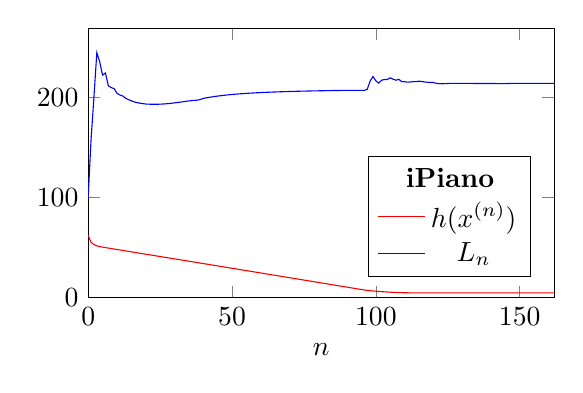
\begin{tikzpicture}
			\begin{axis}[%
					xlabel=$n$,
					xmin=0,
					xmax=162,
					ymin=0,
					height=5cm,
					width=7.5cm,
					legend style={at={(0.95,0.3)},anchor=east}
				]
				\addlegendimage{empty legend}
				\addlegendentry{\hspace{-.6cm}\textbf{iPiano}}
				%  %%%%%%%%%%%%%%%%%%%%%%%%%%%%%%%%%%%%%%%%%%%%%%%%%%%%%%%%%%%%
				\addplot[color=red] coordinates{
					(0,61.9284)
					(1,55.0942)
					(2,52.8104)
					(3,51.5286)
					(4,50.8406)
					(5,50.2876)
					(6,49.7831)
					(7,49.2999)
					(8,48.8285)
					(9,48.3644)
					(10,47.8984)
					(11,47.4317)
					(12,46.965)
					(13,46.4965)
					(14,46.0267)
					(15,45.5559)
					(16,45.0841)
					(17,44.6116)
					(18,44.139)
					(19,43.6663)
					(20,43.1937)
					(21,42.7214)
					(22,42.2497)
					(23,41.7785)
					(24,41.308)
					(25,40.8383)
					(26,40.3693)
					(27,39.901)
					(28,39.4335)
					(29,38.9666)
					(30,38.5003)
					(31,38.0343)
					(32,37.5685)
					(33,37.1025)
					(34,36.6362)
					(35,36.1691)
					(36,35.7009)
					(37,35.2314)
					(38,34.7606)
					(39,34.2897)
					(40,33.8195)
					(41,33.3495)
					(42,32.8795)
					(43,32.4094)
					(44,31.9393)
					(45,31.4692)
					(46,30.9989)
					(47,30.5285)
					(48,30.0581)
					(49,29.5875)
					(50,29.117)
					(51,28.6463)
					(52,28.1756)
					(53,27.7048)
					(54,27.234)
					(55,26.763)
					(56,26.292)
					(57,25.8209)
					(58,25.3498)
					(59,24.8786)
					(60,24.4072)
					(61,23.9358)
					(62,23.4644)
					(63,22.9928)
					(64,22.5212)
					(65,22.0496)
					(66,21.5778)
					(67,21.106)
					(68,20.6341)
					(69,20.1622)
					(70,19.6901)
					(71,19.2181)
					(72,18.7459)
					(73,18.2738)
					(74,17.8015)
					(75,17.3292)
					(76,16.8568)
					(77,16.3844)
					(78,15.9119)
					(79,15.4394)
					(80,14.9668)
					(81,14.4942)
					(82,14.0215)
					(83,13.5487)
					(84,13.0759)
					(85,12.6031)
					(86,12.1302)
					(87,11.6573)
					(88,11.1843)
					(89,10.7113)
					(90,10.2382)
					(91,9.76508)
					(92,9.29182)
					(93,8.81845)
					(94,8.34497)
					(95,7.87138)
					(96,7.40974)
					(97,7.01056)
					(98,6.69462)
					(99,6.42987)
					(100,6.18403)
					(101,5.95454)
					(102,5.74638)
					(103,5.55434)
					(104,5.37824)
					(105,5.21127)
					(106,5.05771)
					(107,4.92417)
					(108,4.80774)
					(109,4.71376)
					(110,4.6422)
					(111,4.59906)
					(112,4.57173)
					(113,4.55306)
					(114,4.53847)
					(115,4.52638)
					(116,4.51568)
					(117,4.50575)
					(118,4.4963)
					(119,4.48724)
					(120,4.4801)
					(121,4.47573)
					(122,4.47269)
					(123,4.47044)
					(124,4.46877)
					(125,4.4675)
					(126,4.4665)
					(127,4.46569)
					(128,4.46501)
					(129,4.46442)
					(130,4.4639)
					(131,4.46345)
					(132,4.46303)
					(133,4.46266)
					(134,4.46231)
					(135,4.462)
					(136,4.46172)
					(137,4.46145)
					(138,4.46121)
					(139,4.46099)
					(140,4.46078)
					(141,4.4606)
					(142,4.46042)
					(143,4.46026)
					(144,4.46012)
					(145,4.46003)
					(146,4.45996)
					(147,4.45992)
					(148,4.45989)
					(149,4.45986)
					(150,4.45985)
					(151,4.45984)
					(152,4.45983)
					(153,4.45982)
					(154,4.45982)
					(155,4.45982)
					(156,4.45981)
					(157,4.45981)
					(158,4.45981)
					(159,4.45981)
					(160,4.45981)
					(161,4.45981)
					(162,4.4598)
				};
				\addlegendentry{$h(x^{(n)})$}
				%-%
				%  %%%%%%%%%%%%%%%%%%%%%%%%%%%%%%%%%%%%%%%%%%%%%%%%%%%%%%%%%%%%
				\addplot[color=blue] coordinates{
					(0,100)
					(1,158.024)
					(2,200.18)
					(3,244.6)
					(4,235.454)
					(5,222.215)
					(6,224.275)
					(7,211.492)
					(8,209.73)
					(9,208.735)
					(10,204.029)
					(11,202.369)
					(12,201.391)
					(13,199.104)
					(14,197.717)
					(15,196.549)
					(16,195.419)
					(17,194.671)
					(18,194.155)
					(19,193.694)
					(20,193.286)
					(21,193.154)
					(22,193.063)
					(23,193.009)
					(24,193.052)
					(25,193.161)
					(26,193.314)
					(27,193.517)
					(28,193.772)
					(29,194.071)
					(30,194.411)
					(31,194.785)
					(32,195.184)
					(33,195.593)
					(34,195.995)
					(35,196.37)
					(36,196.699)
					(37,196.966)
					(38,197.158)
					(39,197.848)
					(40,198.849)
					(41,199.478)
					(42,199.942)
					(43,200.404)
					(44,200.848)
					(45,201.237)
					(46,201.589)
					(47,201.925)
					(48,202.247)
					(49,202.547)
					(50,202.822)
					(51,203.076)
					(52,203.313)
					(53,203.534)
					(54,203.741)
					(55,203.935)
					(56,204.117)
					(57,204.288)
					(58,204.449)
					(59,204.601)
					(60,204.743)
					(61,204.879)
					(62,205.006)
					(63,205.127)
					(64,205.242)
					(65,205.351)
					(66,205.455)
					(67,205.553)
					(68,205.647)
					(69,205.737)
					(70,205.823)
					(71,205.904)
					(72,205.983)
					(73,206.058)
					(74,206.129)
					(75,206.198)
					(76,206.264)
					(77,206.328)
					(78,206.389)
					(79,206.447)
					(80,206.504)
					(81,206.558)
					(82,206.611)
					(83,206.662)
					(84,206.71)
					(85,206.758)
					(86,206.803)
					(87,206.847)
					(88,206.89)
					(89,206.931)
					(90,206.971)
					(91,206.998)
					(92,206.985)
					(93,206.991)
					(94,207.002)
					(95,207.003)
					(96,207.003)
					(97,207.921)
					(98,216.117)
					(99,220.812)
					(100,216.462)
					(101,214.134)
					(102,217.09)
					(103,217.789)
					(104,217.875)
					(105,219.549)
					(106,218.02)
					(107,217.075)
					(108,217.983)
					(109,215.616)
					(110,215.608)
					(111,215.151)
					(112,215.38)
					(113,215.609)
					(114,215.719)
					(115,216.101)
					(116,215.817)
					(117,215.325)
					(118,215.049)
					(119,214.853)
					(120,214.863)
					(121,213.949)
					(122,213.683)
					(123,213.583)
					(124,213.647)
					(125,213.806)
					(126,213.923)
					(127,213.956)
					(128,213.947)
					(129,213.928)
					(130,213.912)
					(131,213.898)
					(132,213.886)
					(133,213.872)
					(134,213.859)
					(135,213.845)
					(136,213.831)
					(137,213.817)
					(138,213.803)
					(139,213.789)
					(140,213.775)
					(141,213.761)
					(142,213.747)
					(143,213.734)
					(144,213.721)
					(145,213.725)
					(146,213.811)
					(147,213.869)
					(148,213.924)
					(149,213.94)
					(150,213.941)
					(151,213.945)
					(152,213.949)
					(153,213.953)
					(154,213.957)
					(155,213.96)
					(156,213.962)
					(157,213.963)
					(158,213.965)
					(159,213.965)
					(160,213.965)
					(161,213.966)
					(162,213.965)
				};
				\addlegendentry{$L_n$}
			\end{axis}
		\end{tikzpicture}
		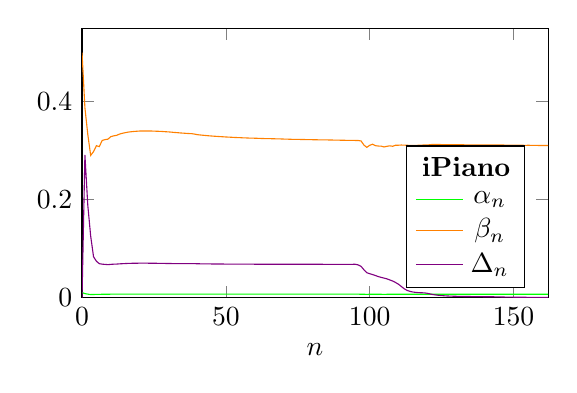
\begin{tikzpicture}
			\begin{axis}[%
					xlabel=$n$,
					xmin=0,
					xmax=162,
					ymin=0,
					height=5cm,
					width=7.5cm,
					legend style={at={(0.95,0.3)},anchor=east}
				]
				\addlegendimage{empty legend}
				\addlegendentry{\hspace{-.6cm}\textbf{iPiano}}
				%-%
				%  %%%%%%%%%%%%%%%%%%%%%%%%%%%%%%%%%%%%%%%%%%%%%%%%%%%%%%%%%%%%
				\addplot[color=green] coordinates{
					(0,0.009999)
					(1,0.00775131)
					(2,0.00666305)
					(3,0.00580436)
					(4,0.0059639)
					(5,0.00620958)
					(6,0.00617039)
					(7,0.00642403)
					(8,0.0064615)
					(9,0.00648293)
					(10,0.00658325)
					(11,0.00662004)
					(12,0.00664176)
					(13,0.00669282)
					(14,0.00672391)
					(15,0.00675074)
					(16,0.00677797)
					(17,0.00679593)
					(18,0.00680846)
					(19,0.00681984)
					(20,0.00683007)
					(21,0.00683349)
					(22,0.00683701)
					(23,0.00683863)
					(24,0.00683797)
					(25,0.00683578)
					(26,0.00683294)
					(27,0.0068281)
					(28,0.00682252)
					(29,0.00681627)
					(30,0.00680829)
					(31,0.00680032)
					(32,0.00679181)
					(33,0.00678263)
					(34,0.00677409)
					(35,0.00676608)
					(36,0.00675889)
					(37,0.00675382)
					(38,0.00674943)
					(39,0.00673411)
					(40,0.00671214)
					(41,0.00669822)
					(42,0.0066885)
					(43,0.0066785)
					(44,0.00666928)
					(45,0.00666095)
					(46,0.00665382)
					(47,0.00664672)
					(48,0.00663993)
					(49,0.00663364)
					(50,0.00662857)
					(51,0.00662332)
					(52,0.00661845)
					(53,0.00661423)
					(54,0.00660988)
					(55,0.00660648)
					(56,0.00660313)
					(57,0.00659992)
					(58,0.00659703)
					(59,0.00659361)
					(60,0.00659114)
					(61,0.00658852)
					(62,0.00658701)
					(63,0.00658471)
					(64,0.00658282)
					(65,0.00658033)
					(66,0.00657809)
					(67,0.00657659)
					(68,0.00657487)
					(69,0.00657356)
					(70,0.00657297)
					(71,0.00657215)
					(72,0.0065714)
					(73,0.00657038)
					(74,0.0065687)
					(75,0.00656816)
					(76,0.00656704)
					(77,0.0065663)
					(78,0.00656561)
					(79,0.00656465)
					(80,0.00656406)
					(81,0.00656351)
					(82,0.006563)
					(83,0.00656223)
					(84,0.00656148)
					(85,0.00656047)
					(86,0.00656011)
					(87,0.00656009)
					(88,0.00656011)
					(89,0.00655984)
					(90,0.0065596)
					(91,0.00656027)
					(92,0.00656117)
					(93,0.00656197)
					(94,0.00656266)
					(95,0.00656326)
					(96,0.00656419)
					(97,0.00654478)
					(98,0.0063741)
					(99,0.00628041)
					(100,0.00636825)
					(101,0.0064164)
					(102,0.00635669)
					(103,0.00634318)
					(104,0.00634258)
					(105,0.00630935)
					(106,0.00634079)
					(107,0.00636013)
					(108,0.0063421)
					(109,0.00639122)
					(110,0.00639138)
					(111,0.0064016)
					(112,0.00639719)
					(113,0.00639252)
					(114,0.00639078)
					(115,0.00638342)
					(116,0.00638972)
					(117,0.00639991)
					(118,0.00640585)
					(119,0.00640989)
					(120,0.00640997)
					(121,0.00642932)
					(122,0.00643467)
					(123,0.00643704)
					(124,0.006436)
					(125,0.00643359)
					(126,0.00643175)
					(127,0.00643135)
					(128,0.00643271)
					(129,0.00643311)
					(130,0.00643373)
					(131,0.00643431)
					(132,0.00643456)
					(133,0.00643571)
					(134,0.00643628)
					(135,0.0064371)
					(136,0.00643746)
					(137,0.0064379)
					(138,0.00643848)
					(139,0.00643906)
					(140,0.00643964)
					(141,0.00644021)
					(142,0.00644137)
					(143,0.00644194)
					(144,0.0064425)
					(145,0.00644271)
					(146,0.00644121)
					(147,0.00644088)
					(148,0.00644004)
					(149,0.00644028)
					(150,0.00644078)
					(151,0.00644112)
					(152,0.00644192)
					(153,0.00644212)
					(154,0.00644256)
					(155,0.00644234)
					(156,0.00644259)
					(157,0.00644372)
					(158,0.00644485)
					(159,0.00644543)
					(160,0.00644571)
					(161,0.00644628)
					(162,0.00644687)
				};
				\addlegendentry{$\alpha_n$}
				%-%
				%  %%%%%%%%%%%%%%%%%%%%%%%%%%%%%%%%%%%%%%%%%%%%%%%%%%%%%%%%%%%%
				\addplot[color=orange] coordinates{
					(0,0.5)
					(1,0.387555)
					(2,0.333094)
					(3,0.290126)
					(4,0.297888)
					(5,0.31007)
					(6,0.308069)
					(7,0.320685)
					(8,0.322413)
					(9,0.323323)
					(10,0.328415)
					(11,0.330086)
					(12,0.331138)
					(13,0.333651)
					(14,0.335285)
					(15,0.336572)
					(16,0.337726)
					(17,0.33845)
					(18,0.339053)
					(19,0.339517)
					(20,0.339923)
					(21,0.340042)
					(22,0.340011)
					(23,0.34004)
					(24,0.339956)
					(25,0.339796)
					(26,0.339483)
					(27,0.339323)
					(28,0.338994)
					(29,0.338513)
					(30,0.338197)
					(31,0.3377)
					(32,0.337107)
					(33,0.336683)
					(34,0.33609)
					(35,0.335673)
					(36,0.335266)
					(37,0.334864)
					(38,0.334646)
					(39,0.333836)
					(40,0.332581)
					(41,0.331926)
					(42,0.331345)
					(43,0.3308)
					(44,0.330245)
					(45,0.329783)
					(46,0.329332)
					(47,0.328932)
					(48,0.328547)
					(49,0.328187)
					(50,0.32779)
					(51,0.327481)
					(52,0.327192)
					(53,0.326822)
					(54,0.32658)
					(55,0.326353)
					(56,0.326027)
					(57,0.325858)
					(58,0.325554)
					(59,0.325472)
					(60,0.325254)
					(61,0.325077)
					(62,0.32481)
					(63,0.324648)
					(64,0.324396)
					(65,0.32436)
					(66,0.32425)
					(67,0.32408)
					(68,0.323947)
					(69,0.323787)
					(70,0.323567)
					(71,0.323383)
					(72,0.323203)
					(73,0.322994)
					(74,0.322999)
					(75,0.322829)
					(76,0.322727)
					(77,0.322595)
					(78,0.322466)
					(79,0.322372)
					(80,0.322248)
					(81,0.322126)
					(82,0.322006)
					(83,0.32192)
					(84,0.321836)
					(85,0.321787)
					(86,0.321674)
					(87,0.321531)
					(88,0.32139)
					(89,0.321282)
					(90,0.321176)
					(91,0.321019)
					(92,0.320969)
					(93,0.320866)
					(94,0.320758)
					(95,0.320693)
					(96,0.320597)
					(97,0.319603)
					(98,0.311223)
					(99,0.306604)
					(100,0.310757)
					(101,0.313016)
					(102,0.310013)
					(103,0.309264)
					(104,0.309056)
					(105,0.307393)
					(106,0.308791)
					(107,0.309688)
					(108,0.308765)
					(109,0.310976)
					(110,0.310984)
					(111,0.311345)
					(112,0.311086)
					(113,0.310859)
					(114,0.310625)
					(115,0.31027)
					(116,0.310427)
					(117,0.310969)
					(118,0.311213)
					(119,0.311409)
					(120,0.311368)
					(121,0.312158)
					(122,0.31251)
					(123,0.31258)
					(124,0.312484)
					(125,0.312231)
					(126,0.312051)
					(127,0.311986)
					(128,0.311871)
					(129,0.31189)
					(130,0.311875)
					(131,0.311858)
					(132,0.31187)
					(133,0.311789)
					(134,0.311772)
					(135,0.311662)
					(136,0.311667)
					(137,0.311735)
					(138,0.311718)
					(139,0.311701)
					(140,0.311684)
					(141,0.311667)
					(142,0.311587)
					(143,0.31157)
					(144,0.311551)
					(145,0.311516)
					(146,0.311399)
					(147,0.311247)
					(148,0.311162)
					(149,0.311083)
					(150,0.310958)
					(151,0.310976)
					(152,0.31088)
					(153,0.310844)
					(154,0.310716)
					(155,0.310799)
					(156,0.310765)
					(157,0.31064)
					(158,0.310514)
					(159,0.310452)
					(160,0.310421)
					(161,0.310358)
					(162,0.310297)
				};
				\addlegendentry{$\beta_n$}
				%-%
				%  %%%%%%%%%%%%%%%%%%%%%%%%%%%%%%%%%%%%%%%%%%%%%%%%%%%%%%%%%%%%
				\addplot[color=violet] coordinates{
					(0,-0.000364599)
					(1,0.29112)
					(2,0.188431)
					(3,0.125521)
					(4,0.0830333)
					(5,0.0738709)
					(6,0.0689289)
					(7,0.0679369)
					(8,0.0674423)
					(9,0.0669165)
					(10,0.0675091)
					(11,0.0678859)
					(12,0.0680741)
					(13,0.0685265)
					(14,0.068883)
					(15,0.0691719)
					(16,0.0694485)
					(17,0.0696419)
					(18,0.0697675)
					(19,0.0698584)
					(20,0.069932)
					(21,0.0699415)
					(22,0.0699245)
					(23,0.0698944)
					(24,0.0698413)
					(25,0.0697695)
					(26,0.0696822)
					(27,0.0695926)
					(28,0.0694934)
					(29,0.0693844)
					(30,0.0692828)
					(31,0.0691834)
					(32,0.0690892)
					(33,0.0690188)
					(34,0.0689643)
					(35,0.0689455)
					(36,0.068956)
					(37,0.0689982)
					(38,0.0690541)
					(39,0.0689863)
					(40,0.0687915)
					(41,0.0686534)
					(42,0.0685653)
					(43,0.0684898)
					(44,0.068418)
					(45,0.0683561)
					(46,0.0683031)
					(47,0.068253)
					(48,0.0682046)
					(49,0.0681588)
					(50,0.0681174)
					(51,0.0680799)
					(52,0.0680456)
					(53,0.0680094)
					(54,0.0679789)
					(55,0.0679562)
					(56,0.067928)
					(57,0.0679085)
					(58,0.0678839)
					(59,0.0678676)
					(60,0.0678502)
					(61,0.0678335)
					(62,0.0678178)
					(63,0.0678029)
					(64,0.0677843)
					(65,0.0677743)
					(66,0.0677632)
					(67,0.0677522)
					(68,0.0677416)
					(69,0.0677315)
					(70,0.0677219)
					(71,0.0677132)
					(72,0.0677048)
					(73,0.0676922)
					(74,0.0676878)
					(75,0.0676818)
					(76,0.0676753)
					(77,0.067669)
					(78,0.067663)
					(79,0.0676574)
					(80,0.0676521)
					(81,0.0676469)
					(82,0.067642)
					(83,0.0676373)
					(84,0.0676328)
					(85,0.0676285)
					(86,0.0676244)
					(87,0.0676206)
					(88,0.0676168)
					(89,0.0676135)
					(90,0.0676101)
					(91,0.0676095)
					(92,0.0676185)
					(93,0.0676263)
					(94,0.0676323)
					(95,0.0676399)
					(96,0.0664473)
					(97,0.0634335)
					(98,0.0563558)
					(99,0.0504509)
					(100,0.0484512)
					(101,0.0466692)
					(102,0.044658)
					(103,0.0425239)
					(104,0.0408775)
					(105,0.0394562)
					(106,0.0378493)
					(107,0.0356754)
					(108,0.033438)
					(109,0.0304092)
					(110,0.0269292)
					(111,0.0222727)
					(112,0.0176444)
					(113,0.01427)
					(114,0.0122985)
					(115,0.0110299)
					(116,0.0102373)
					(117,0.00975667)
					(118,0.00947644)
					(119,0.00927437)
					(120,0.00838955)
					(121,0.00705895)
					(122,0.00581927)
					(123,0.00495177)
					(124,0.0042562)
					(125,0.00368505)
					(126,0.00323513)
					(127,0.00289348)
					(128,0.00263187)
					(129,0.00242761)
					(130,0.00226444)
					(131,0.00213028)
					(132,0.00201653)
					(133,0.00191723)
					(134,0.0018283)
					(135,0.00174697)
					(136,0.00167164)
					(137,0.00160121)
					(138,0.00153457)
					(139,0.00147132)
					(140,0.00141093)
					(141,0.0013532)
					(142,0.00129802)
					(143,0.00124511)
					(144,0.00116703)
					(145,0.00102722)
					(146,0.000853786)
					(147,0.00070983)
					(148,0.000591104)
					(149,0.000493866)
					(150,0.000414036)
					(151,0.000348762)
					(152,0.000295921)
					(153,0.000253343)
					(154,0.000219127)
					(155,0.000191635)
					(156,0.000169635)
					(157,0.000151994)
					(158,0.000137841)
					(159,0.000126463)
					(160,0.000117236)
					(161,0.000109609)
					(162,0.00010332)
				};
				\addlegendentry{$\Delta_n$}
				%/%
			\end{axis}
		\end{tikzpicture}
	\end{subfigure}
	\begin{subfigure}[t]{0.85\textwidth}
		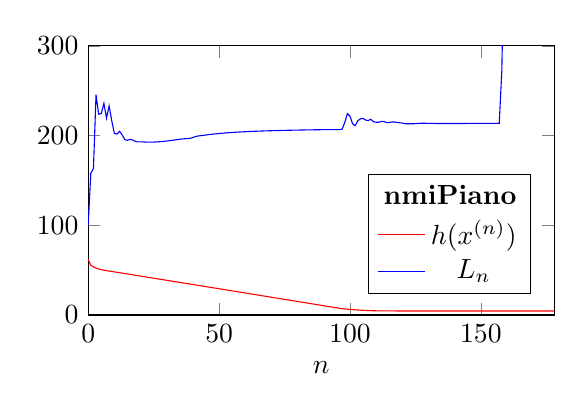
\begin{tikzpicture}
			\begin{axis}[%
					xlabel=$n$,
					xmin=0,
					xmax=178,
					ymin=0,
					ymax=300,
					height=5cm,
					width=7.5cm,
					legend style={at={(0.95,0.3)},anchor=east}
				]
				\addlegendimage{empty legend}
				\addlegendentry{\hspace{-.6cm}\textbf{nmiPiano}}
				%  %%%%%%%%%%%%%%%%%%%%%%%%%%%%%%%%%%%%%%%%%%%%%%%%%%%%%%%%%%%%
				\addplot[color=red] coordinates{
					(0,61.9284)
					(1,55.4126)
					(2,53.5439)
					(3,52.2985)
					(4,51.1704)
					(5,50.5461)
					(6,49.9138)
					(7,49.4093)
					(8,48.9473)
					(9,48.4961)
					(10,48.0341)
					(11,47.5708)
					(12,47.11)
					(13,46.6471)
					(14,46.1779)
					(15,45.7057)
					(16,45.2339)
					(17,44.7621)
					(18,44.289)
					(19,43.8152)
					(20,43.3416)
					(21,42.8684)
					(22,42.3957)
					(23,41.9234)
					(24,41.4517)
					(25,40.9806)
					(26,40.5102)
					(27,40.0405)
					(28,39.5715)
					(29,39.1031)
					(30,38.6353)
					(31,38.168)
					(32,37.7009)
					(33,37.2338)
					(34,36.7665)
					(35,36.2986)
					(36,35.8298)
					(37,35.36)
					(38,34.8887)
					(39,34.4164)
					(40,33.9441)
					(41,33.4725)
					(42,33.0012)
					(43,32.5299)
					(44,32.0586)
					(45,31.5871)
					(46,31.1155)
					(47,30.6439)
					(48,30.1722)
					(49,29.7004)
					(50,29.2285)
					(51,28.7566)
					(52,28.2846)
					(53,27.8127)
					(54,27.3406)
					(55,26.8685)
					(56,26.3964)
					(57,25.9241)
					(58,25.4519)
					(59,24.9795)
					(60,24.5071)
					(61,24.0346)
					(62,23.5621)
					(63,23.0895)
					(64,22.6168)
					(65,22.1441)
					(66,21.6713)
					(67,21.1985)
					(68,20.7256)
					(69,20.2527)
					(70,19.7796)
					(71,19.3066)
					(72,18.8334)
					(73,18.3603)
					(74,17.887)
					(75,17.4137)
					(76,16.9404)
					(77,16.467)
					(78,15.9935)
					(79,15.52)
					(80,15.0465)
					(81,14.5729)
					(82,14.0992)
					(83,13.6255)
					(84,13.1518)
					(85,12.678)
					(86,12.2041)
					(87,11.7303)
					(88,11.2563)
					(89,10.7824)
					(90,10.3084)
					(91,9.8343)
					(92,9.36015)
					(93,8.88588)
					(94,8.4115)
					(95,7.937)
					(96,7.46982)
					(97,7.06011)
					(98,6.73075)
					(99,6.45856)
					(100,6.20925)
					(101,5.97619)
					(102,5.76138)
					(103,5.56307)
					(104,5.38394)
					(105,5.21463)
					(106,5.05718)
					(107,4.92203)
					(108,4.80652)
					(109,4.71057)
					(110,4.63754)
					(111,4.59357)
					(112,4.56691)
					(113,4.54751)
					(114,4.53325)
					(115,4.52125)
					(116,4.51073)
					(117,4.50093)
					(118,4.49165)
					(119,4.48297)
					(120,4.47718)
					(121,4.4735)
					(122,4.47078)
					(123,4.46873)
					(124,4.46723)
					(125,4.46613)
					(126,4.46529)
					(127,4.46463)
					(128,4.46406)
					(129,4.46357)
					(130,4.46314)
					(131,4.46275)
					(132,4.46239)
					(133,4.46207)
					(134,4.46177)
					(135,4.46149)
					(136,4.46124)
					(137,4.46101)
					(138,4.4608)
					(139,4.46061)
					(140,4.46043)
					(141,4.46027)
					(142,4.46012)
					(143,4.46003)
					(144,4.45996)
					(145,4.45991)
					(146,4.45988)
					(147,4.45986)
					(148,4.45984)
					(149,4.45983)
					(150,4.45983)
					(151,4.45982)
					(152,4.45982)
					(153,4.45982)
					(154,4.45981)
					(155,4.45981)
					(156,4.45981)
					(157,4.45981)
					(158,4.45981)
					(159,4.45981)
					(160,4.45981)
					(161,4.45981)
					(162,4.45981)
					(163,4.45981)
					(164,4.45981)
					(165,4.45981)
					(166,4.4598)
					(167,4.45981)
					(168,4.45981)
					(169,4.45981)
					(170,4.45981)
					(171,4.4598)
					(172,4.4598)
					(173,4.45981)
					(174,4.45981)
					(175,4.4598)
					(176,4.45981)
					(177,4.45981)
					(178,4.4598)
				};
				\addlegendentry{$h(x^{(n)})$}
				%-%
				%  %%%%%%%%%%%%%%%%%%%%%%%%%%%%%%%%%%%%%%%%%%%%%%%%%%%%%%%%%%%%
				\addplot[color=blue] coordinates{
					(0,100)
					(1,158.022)
					(2,163.105)
					(3,245.471)
					(4,223.818)
					(5,224.457)
					(6,235.909)
					(7,219.423)
					(8,232.985)
					(9,216.391)
					(10,202.322)
					(11,201.656)
					(12,204.718)
					(13,200.646)
					(14,195.348)
					(15,194.725)
					(16,195.739)
					(17,194.992)
					(18,193.496)
					(19,192.872)
					(20,192.876)
					(21,192.861)
					(22,192.72)
					(23,192.631)
					(24,192.644)
					(25,192.715)
					(26,192.843)
					(27,193.037)
					(28,193.283)
					(29,193.571)
					(30,193.9)
					(31,194.266)
					(32,194.655)
					(33,195.055)
					(34,195.454)
					(35,195.838)
					(36,196.186)
					(37,196.479)
					(38,196.706)
					(39,196.858)
					(40,197.778)
					(41,198.84)
					(42,199.506)
					(43,199.892)
					(44,200.234)
					(45,200.619)
					(46,201.012)
					(47,201.362)
					(48,201.665)
					(49,201.948)
					(50,202.232)
					(51,202.515)
					(52,202.781)
					(53,203.02)
					(54,203.233)
					(55,203.428)
					(56,203.612)
					(57,203.788)
					(58,203.956)
					(59,204.115)
					(60,204.264)
					(61,204.404)
					(62,204.536)
					(63,204.661)
					(64,204.78)
					(65,204.892)
					(66,204.999)
					(67,205.101)
					(68,205.198)
					(69,205.29)
					(70,205.379)
					(71,205.463)
					(72,205.543)
					(73,205.62)
					(74,205.694)
					(75,205.765)
					(76,205.832)
					(77,205.898)
					(78,205.96)
					(79,206.02)
					(80,206.078)
					(81,206.134)
					(82,206.187)
					(83,206.239)
					(84,206.289)
					(85,206.337)
					(86,206.383)
					(87,206.428)
					(88,206.472)
					(89,206.514)
					(90,206.554)
					(91,206.593)
					(92,206.589)
					(93,206.575)
					(94,206.581)
					(95,206.596)
					(96,206.601)
					(97,207.038)
					(98,214.594)
					(99,224.436)
					(100,221.511)
					(101,213.071)
					(102,210.916)
					(103,216.564)
					(104,218.603)
					(105,219.068)
					(106,217.188)
					(107,216.695)
					(108,218.121)
					(109,215.279)
					(110,214.852)
					(111,214.848)
					(112,215.754)
					(113,215.737)
					(114,214.376)
					(115,214.515)
					(116,215.093)
					(117,215.123)
					(118,214.562)
					(119,214.168)
					(120,213.907)
					(121,213.174)
					(122,213.11)
					(123,213.069)
					(124,213.098)
					(125,213.267)
					(126,213.492)
					(127,213.645)
					(128,213.682)
					(129,213.638)
					(130,213.57)
					(131,213.514)
					(132,213.481)
					(133,213.467)
					(134,213.462)
					(135,213.454)
					(136,213.443)
					(137,213.429)
					(138,213.414)
					(139,213.4)
					(140,213.384)
					(141,213.37)
					(142,213.356)
					(143,213.367)
					(144,213.463)
					(145,213.53)
					(146,213.582)
					(147,213.619)
					(148,213.628)
					(149,213.616)
					(150,213.605)
					(151,213.605)
					(152,213.608)
					(153,213.611)
					(154,213.614)
					(155,213.618)
					(156,213.62)
					(157,213.62)
					(158,272.639)
					(159,442.824)
					(160,1111.91)
					(161,1551.01)
					(162,2647.69)
					(163,1877.73)
					(164,2176.37)
					(165,1623.11)
					(166,3724.77)
					(167,3537.62)
					(168,1701.84)
					(169,4105.64)
					(170,2393.89)
					(171,7012.66)
					(172,2391.9)
					(173,27490.6)
					(174,2766.56)
					(175,8946.06)
					(176,3709.78)
					(177,9386.35)
					(178,6042.67)
				};
				\addlegendentry{$L_n$}
			\end{axis}
		\end{tikzpicture}
		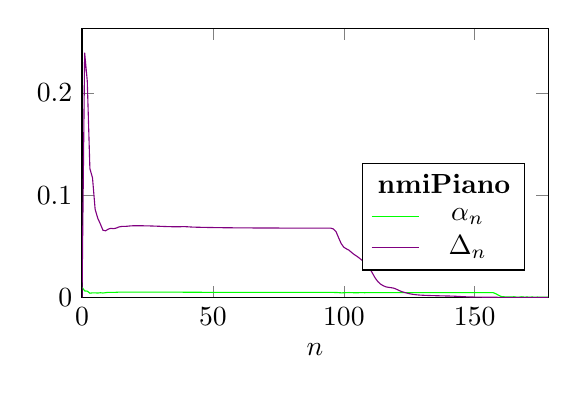
\begin{tikzpicture}
			\begin{axis}[%
					xlabel=$n$,
					xmin=0,
					xmax=178,
					ymin=0,
					height=5cm,
					width=7.5cm,
					legend style={at={(0.95,0.3)},anchor=east}
				]
				\addlegendimage{empty legend}
				\addlegendentry{\hspace{-.6cm}\textbf{nmiPiano}}
				%-%
				%  %%%%%%%%%%%%%%%%%%%%%%%%%%%%%%%%%%%%%%%%%%%%%%%%%%%%%%%%%%%%
				\addplot[color=green] coordinates{
					(0,0.01)
					(1,0.00632824)
					(2,0.00613102)
					(3,0.00407379)
					(4,0.00446791)
					(5,0.0044552)
					(6,0.00423893)
					(7,0.00455741)
					(8,0.00429212)
					(9,0.00462127)
					(10,0.00494262)
					(11,0.00495894)
					(12,0.00488476)
					(13,0.00498389)
					(14,0.00511907)
					(15,0.00513545)
					(16,0.00510885)
					(17,0.0051284)
					(18,0.00516806)
					(19,0.0051848)
					(20,0.00518467)
					(21,0.00518508)
					(22,0.00518888)
					(23,0.00519128)
					(24,0.00519092)
					(25,0.005189)
					(26,0.00518557)
					(27,0.00518035)
					(28,0.00517375)
					(29,0.00516607)
					(30,0.0051573)
					(31,0.00514759)
					(32,0.0051373)
					(33,0.00512677)
					(34,0.00511628)
					(35,0.00510626)
					(36,0.00509722)
					(37,0.0050896)
					(38,0.00508372)
					(39,0.00507981)
					(40,0.00505616)
					(41,0.00502918)
					(42,0.00501237)
					(43,0.00500271)
					(44,0.00499416)
					(45,0.00498456)
					(46,0.00497483)
					(47,0.00496619)
					(48,0.00495873)
					(49,0.00495178)
					(50,0.00494482)
					(51,0.00493791)
					(52,0.00493142)
					(53,0.00492561)
					(54,0.00492045)
					(55,0.00491575)
					(56,0.00491131)
					(57,0.00490706)
					(58,0.00490302)
					(59,0.00489921)
					(60,0.00489564)
					(61,0.00489228)
					(62,0.00488912)
					(63,0.00488613)
					(64,0.0048833)
					(65,0.00488061)
					(66,0.00487806)
					(67,0.00487564)
					(68,0.00487334)
					(69,0.00487115)
					(70,0.00486906)
					(71,0.00486706)
					(72,0.00486515)
					(73,0.00486333)
					(74,0.00486159)
					(75,0.00485992)
					(76,0.00485832)
					(77,0.00485678)
					(78,0.00485531)
					(79,0.00485389)
					(80,0.00485253)
					(81,0.00485122)
					(82,0.00484996)
					(83,0.00484874)
					(84,0.00484757)
					(85,0.00484644)
					(86,0.00484535)
					(87,0.0048443)
					(88,0.00484328)
					(89,0.00484229)
					(90,0.00484134)
					(91,0.00484044)
					(92,0.00484053)
					(93,0.00484085)
					(94,0.00484071)
					(95,0.00484037)
					(96,0.00484024)
					(97,0.00483002)
					(98,0.00465997)
					(99,0.00445561)
					(100,0.00451445)
					(101,0.00469327)
					(102,0.00474123)
					(103,0.00461757)
					(104,0.00457451)
					(105,0.00456479)
					(106,0.00460431)
					(107,0.00461477)
					(108,0.0045846)
					(109,0.00464514)
					(110,0.00465438)
					(111,0.00465445)
					(112,0.00463491)
					(113,0.00463526)
					(114,0.0046647)
					(115,0.00466168)
					(116,0.00464915)
					(117,0.0046485)
					(118,0.00466067)
					(119,0.00466924)
					(120,0.00467492)
					(121,0.00469101)
					(122,0.00469241)
					(123,0.00469332)
					(124,0.00469267)
					(125,0.00468895)
					(126,0.00468401)
					(127,0.00468066)
					(128,0.00467986)
					(129,0.00468081)
					(130,0.00468231)
					(131,0.00468354)
					(132,0.00468426)
					(133,0.00468457)
					(134,0.00468468)
					(135,0.00468484)
					(136,0.00468508)
					(137,0.00468539)
					(138,0.00468572)
					(139,0.00468605)
					(140,0.00468638)
					(141,0.0046867)
					(142,0.004687)
					(143,0.00468677)
					(144,0.00468466)
					(145,0.00468319)
					(146,0.00468205)
					(147,0.00468123)
					(148,0.00468103)
					(149,0.00468129)
					(150,0.00468153)
					(151,0.00468155)
					(152,0.00468147)
					(153,0.0046814)
					(154,0.00468133)
					(155,0.00468125)
					(156,0.00468121)
					(157,0.0046812)
					(158,0.00366786)
					(159,0.00225823)
					(160,0.000899355)
					(161,0.000644742)
					(162,0.000377687)
					(163,0.000532559)
					(164,0.000459481)
					(165,0.0006161)
					(166,0.000268473)
					(167,0.000282676)
					(168,0.000587599)
					(169,0.000243567)
					(170,0.00041773)
					(171,0.000142599)
					(172,0.000418078)
					(173,3.63761E-005)
					(174,0.00036146)
					(175,0.000111781)
					(176,0.000269558)
					(177,0.000106538)
					(178,0.00016549)
				};
				\addlegendentry{$\alpha_n$}
				%-%
				%  %%%%%%%%%%%%%%%%%%%%%%%%%%%%%%%%%%%%%%%%%%%%%%%%%%%%%%%%%%%%
				\addplot[color=violet] coordinates{
					(0,4.53227E-038)
					(1,0.23935)
					(2,0.211712)
					(3,0.125983)
					(4,0.116887)
					(5,0.0861964)
					(6,0.0774645)
					(7,0.0717913)
					(8,0.0656478)
					(9,0.0651478)
					(10,0.0667587)
					(11,0.0675469)
					(12,0.0672365)
					(13,0.0677334)
					(14,0.0688017)
					(15,0.0693876)
					(16,0.0694322)
					(17,0.0695386)
					(18,0.0698101)
					(19,0.0700127)
					(20,0.0700721)
					(21,0.0700687)
					(22,0.0700606)
					(23,0.0700441)
					(24,0.0700082)
					(25,0.0699558)
					(26,0.0698885)
					(27,0.0698066)
					(28,0.0697129)
					(29,0.0696124)
					(30,0.0695087)
					(31,0.0694055)
					(32,0.069309)
					(33,0.0692247)
					(34,0.0691583)
					(35,0.0691148)
					(36,0.0690987)
					(37,0.0691127)
					(38,0.0691576)
					(39,0.0692094)
					(40,0.0691258)
					(41,0.0689454)
					(42,0.0687895)
					(43,0.0686926)
					(44,0.0686287)
					(45,0.06857)
					(46,0.0685099)
					(47,0.0684541)
					(48,0.0684062)
					(49,0.0683635)
					(50,0.0683213)
					(51,0.0682781)
					(52,0.0682357)
					(53,0.0681967)
					(54,0.0681628)
					(55,0.0681331)
					(56,0.0681062)
					(57,0.0680812)
					(58,0.0680574)
					(59,0.068035)
					(60,0.0680141)
					(61,0.0679949)
					(62,0.067977)
					(63,0.0679603)
					(64,0.0679446)
					(65,0.0679301)
					(66,0.0679166)
					(67,0.0679036)
					(68,0.0678917)
					(69,0.0678807)
					(70,0.06787)
					(71,0.06786)
					(72,0.0678507)
					(73,0.0678419)
					(74,0.0678336)
					(75,0.0678259)
					(76,0.0678184)
					(77,0.0678114)
					(78,0.0678047)
					(79,0.0677985)
					(80,0.0677925)
					(81,0.0677869)
					(82,0.0677815)
					(83,0.0677764)
					(84,0.0677716)
					(85,0.067767)
					(86,0.0677625)
					(87,0.0677584)
					(88,0.0677544)
					(89,0.0677504)
					(90,0.0677467)
					(91,0.0677434)
					(92,0.0677472)
					(93,0.0677559)
					(94,0.0677638)
					(95,0.0677697)
					(96,0.066945)
					(97,0.0644225)
					(98,0.0583232)
					(99,0.0525208)
					(100,0.0490522)
					(101,0.0474738)
					(102,0.0461043)
					(103,0.0438688)
					(104,0.0418333)
					(105,0.0402151)
					(106,0.0382715)
					(107,0.0362116)
					(108,0.0338)
					(109,0.030984)
					(110,0.0278219)
					(111,0.0233015)
					(112,0.0188256)
					(113,0.0154167)
					(114,0.0130498)
					(115,0.011472)
					(116,0.0103807)
					(117,0.00984423)
					(118,0.00951737)
					(119,0.00907964)
					(120,0.00809702)
					(121,0.00685221)
					(122,0.00576316)
					(123,0.0049593)
					(124,0.00426882)
					(125,0.00365242)
					(126,0.00314059)
					(127,0.00275009)
					(128,0.00247395)
					(129,0.00227519)
					(130,0.0021214)
					(131,0.00199787)
					(132,0.001896)
					(133,0.00180778)
					(134,0.00172795)
					(135,0.00165381)
					(136,0.00158395)
					(137,0.00151765)
					(138,0.00145439)
					(139,0.00139383)
					(140,0.00133581)
					(141,0.00128017)
					(142,0.00119185)
					(143,0.00105644)
					(144,0.000902335)
					(145,0.000762624)
					(146,0.000638193)
					(147,0.000530488)
					(148,0.000439158)
					(149,0.000363253)
					(150,0.00030091)
					(151,0.00025162)
					(152,0.000213847)
					(153,0.000185139)
					(154,0.000163214)
					(155,0.000146484)
					(156,0.000133724)
					(157,0.000123884)
					(158,0.000104355)
					(159,7.72046E-005)
					(160,4.82765E-005)
					(161,3.09715E-005)
					(162,1.94378E-005)
					(163,1.52448E-005)
					(164,0.000012374)
					(165,1.25479E-005)
					(166,0.000009033)
					(167,0.000007428)
					(168,9.70836E-006)
					(169,7.33691E-006)
					(170,7.90323E-006)
					(171,5.39419E-006)
					(172,6.92562E-006)
					(173,3.83491E-006)
					(174,5.55453E-006)
					(175,3.91657E-006)
					(176,4.66735E-006)
					(177,3.41347E-006)
					(178,3.37153E-006)
				};
				\addlegendentry{$\Delta_n$}
				%/%
			\end{axis}
		\end{tikzpicture}
	\end{subfigure}
	\caption{Convergence of \textbf{iPiano}, \ie Algorithm \ref{alg:ipiano}, and \textbf{nmiPiano}, \ie Algorithm \ref{alg:nmipiano}. Shown is the value of the objective function $h(x{(n)})$ for each iterate $x{(n)}$, $n \geq 0$, as well as the corresponding parameters $\alpha_n$, $\beta_n$ and $L_n$. For \textbf{nmiPiano} we set $\beta = 0.5$. Furthermore, $\Delta_n := \|x^{(n)} - x^{(n - 1)}\|_2$ is shown.}
	\label{fig:signal-convergence}
\end{figure}

Discretization of the Markov Random Field model of Equation \eqref{eq:mrf} is straight forward:
\begin{align}
	h(\tilde{u}; u^{(0)}, \lambda) = \underbrace{\sum_{i = 1}^n \sum_{j = 1}^m \rho_1(\tilde{u}_{i, j} - \tilde{u}^{(0)}_{i,j})}_{= g(\tilde{u}; u^{(0)})} + \underbrace{\lambda\left[\sum_{i = 2}^n \sum_{j = 1}^m \rho_2(|\tilde{u}_{i,j} - \tilde{u}_{i - 1,j}|) + \sum_{i = 1}^n \sum_{j = 2}^m \rho_2(|\tilde{u}_{i,j} - \tilde{u}_{i,j - 1}|)\right]}_{= f(\tilde{u})}.
\end{align}
While differentiation is linear, leading to an easy-to-compute gradient $\nabla f$, we use the following lemma to compute $\prox{\alpha g}$ in practice:

\begin{lemmamd}
	For $x \in \mathbb{R}^{n \times m}$ and 
	\begin{align}
		g(x) = \sum_{i = 1}^n \sum_{j = 1}^m \rho(x_{i,j})
	\end{align}
	it holds $\prox{\alpha g} \in \mathbb{R}^{n \times m}$ and
	\begin{align}
		\left(\prox{\alpha g}\right)_{i,j} = \prox{\alpha \rho}(x_{i,j}).
	\end{align}
\end{lemmamd}

\subsubsection{Experiments}

In order to discuss convergence as well as the advantage of using $\rho_{1,\text{abs}}$, we first discuss signal denoising (\ie one-dimensional denoising). Figure \ref{fig:signal-convergence} shows the convergence of Algorithms \ref{alg:ipiano} and \ref{alg:nmipiano} for $\rho_{1,\text{abs}}$. Both algorithms converge to $h(x^\ast) := 4.4598$, however, Algorithm \ref{alg:ipiano} converges faster, needing only $162$ iterations compared to $178$ iterations needed for Algrithm \ref{alg:nmipiano} to converge. Of course, this may be due to a suboptimal choice of $\beta = 0.5$ for Algorithm \ref{alg:nmipiano}. On the other hand, this illustrates that automatically adapting both $\alpha_n$ and $\beta_n$ is beneficial. Figure \ref{fig:signal-denoising} shows a signal, the corresponding perturbed/noisy signal and results of using Algorithm \ref{alg:ipiano} for denoising using $\rho_{1,\text{abs}}$ and $\rho_{1,\text{sqr}}$ with different values of~$\lambda$. Gaussian additive noise with standard deviation $\sigma = 0.05$ has been used. The advantage of using $\rho_{1,\text{abs}}$ gets apparent for $\lambda > 0.2$ where the sharp edge is not preserved when using~$\rho_{1, \text{sqr}}$.

\begin{figure}[t]
	\centering
	\begin{subfigure}[t]{0.08\textwidth}
		
\includegraphics[scale=0.3]{pictures/denoising/signal/signal.png}
	\end{subfigure}
	\begin{subfigure}[t]{0.08\textwidth}
		
\includegraphics[scale=0.3]{pictures/denoising/signal/perturbed_signal.png}
	\end{subfigure}
	\begin{subfigure}[t]{0.08\textwidth}
		
\includegraphics[scale=0.3]{pictures/denoising/signal/ipiano_absolute_02.png}
		\scriptsize $\rho_{1,\text{abs}}$\\[2px]
		\scriptsize $\lambda = \frac{1}{0.2}$
	\end{subfigure}
	\begin{subfigure}[t]{0.08\textwidth}
		
\includegraphics[scale=0.3]{pictures/denoising/signal/ipiano_squared_02.png}
		\scriptsize $\rho_{1,\text{sqr}}$\\[2px]
		\scriptsize $\lambda = \frac{1}{0.2}$
	\end{subfigure}
	\begin{subfigure}[t]{0.08\textwidth}
		
\includegraphics[scale=0.3]{pictures/denoising/signal/ipiano_absolute_04.png}
		\scriptsize $\rho_{1,\text{abs}}$\\[2px]
		\scriptsize $\lambda = \frac{1}{0.4}$
	\end{subfigure}
	\begin{subfigure}[t]{0.08\textwidth}
		
\includegraphics[scale=0.3]{pictures/denoising/signal/ipiano_squared_04.png}
		\scriptsize $\rho_{1,\text{sqr}}$\\[2px]
		\scriptsize $\lambda = \frac{1}{0.4}$
	\end{subfigure}
	\begin{subfigure}[t]{0.08\textwidth}
		
\includegraphics[scale=0.3]{pictures/denoising/signal/ipiano_absolute_06.png}
		\scriptsize $\rho_{1,\text{abs}}$\\[2px]
		\scriptsize $\lambda = \frac{1}{0.6}$
	\end{subfigure}
	\begin{subfigure}[t]{0.08\textwidth}
		
\includegraphics[scale=0.3]{pictures/denoising/signal/ipiano_squared_06.png}
		\scriptsize $\rho_{1,\text{sqr}}$\\[2px]
		\scriptsize $\lambda = \frac{1}{0.6}$
	\end{subfigure}
	\begin{subfigure}[t]{0.08\textwidth}
		
\includegraphics[scale=0.3]{pictures/denoising/signal/ipiano_absolute_08.png}
		\scriptsize $\rho_{1,\text{abs}}$\\[2px]
		\scriptsize $\lambda = \frac{1}{0.8}$
	\end{subfigure}
	\begin{subfigure}[t]{0.08\textwidth}
		
\includegraphics[scale=0.3]{pictures/denoising/signal/ipiano_squared_08.png}
		\scriptsize $\rho_{1,\text{sqr}}$\\[2px]
		\scriptsize $\lambda = \frac{1}{0.8}$
	\end{subfigure}
	\caption{Simple signal denoising experiment; input signal shown on the left with the perturbed/noisy signal on its right. The result of applying Algorithm \ref{alg:ipiano} to the proposed denoising model using $\rho_{1, \text{abs}}$ and $\rho_{1,\text{sqr}}$ with $\lambda \in \{\frac{1}{0.2},\frac{1}{0.4},\frac{1}{0.6},\frac{1}{0.8}\}$ is shown.}
	\label{fig:signal-denoising}
\end{figure}

Results of applying Algorithm \ref{alg:ipiano} to denoise images from the Berkeley Segmentation Dataset \cite{ArbelaezMaireFowlkesMalik:2011} are shown in Figure \ref{fig:image-denoising}. Gaussian additive noise with standard deviation $\sigma = 0.05$ has been used. Again, $\rho_{1,\text{sqr}}$ is not able to preserve edges.

\begin{figure}[h]
	\centering
	\begin{subfigure}[t]{0.19\textwidth}
		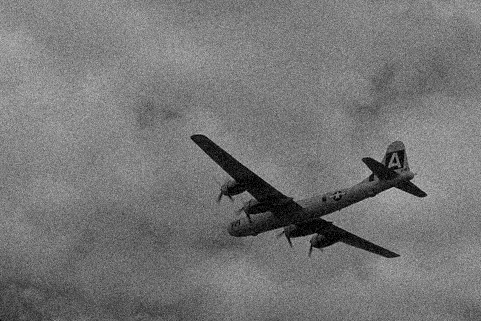
\includegraphics[scale=0.175]{pictures/denoising/image/3096_tilde.png}
	\end{subfigure}
	\begin{subfigure}[t]{0.19\textwidth}
		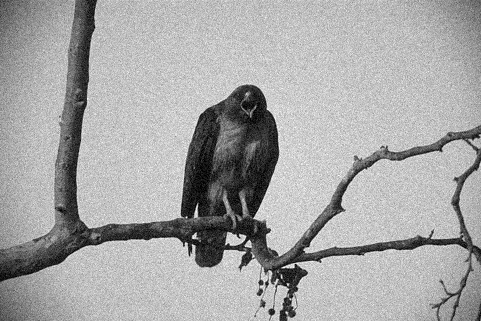
\includegraphics[scale=0.175]{pictures/denoising/image/42049_tilde.png}
	\end{subfigure}
	\begin{subfigure}[t]{0.19\textwidth}
		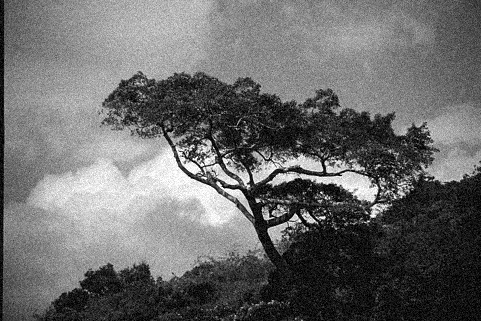
\includegraphics[scale=0.175]{pictures/denoising/image/147091_tilde.png}
	\end{subfigure}
	\begin{subfigure}[t]{0.19\textwidth}
		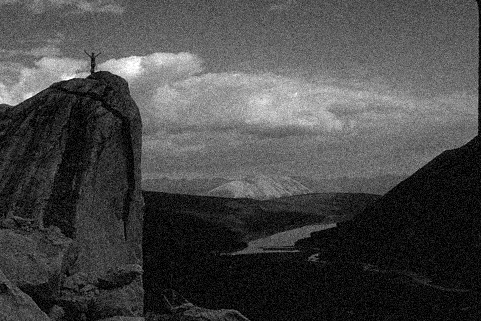
\includegraphics[scale=0.175]{pictures/denoising/image/14037_tilde.png}
	\end{subfigure}
	\begin{subfigure}[t]{0.19\textwidth}
		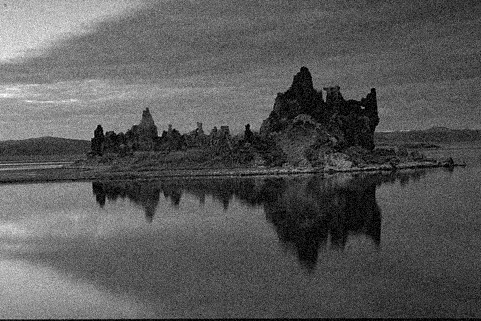
\includegraphics[scale=0.175]{pictures/denoising/image/143090_tilde.png}
	\end{subfigure}
	\begin{subfigure}[t]{0.19\textwidth}
		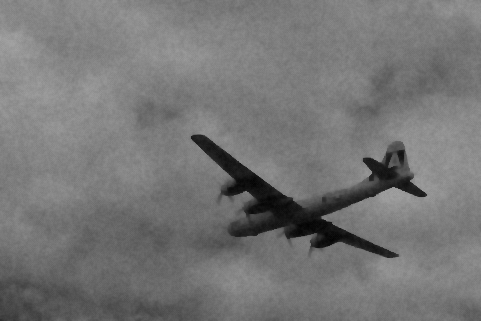
\includegraphics[scale=0.175]{pictures/denoising/image/3096_ipiano_absolute.png}
	\end{subfigure}
	\begin{subfigure}[t]{0.19\textwidth}
		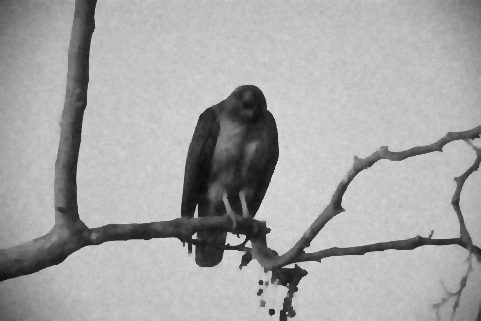
\includegraphics[scale=0.175]{pictures/denoising/image/42049_ipiano_absolute.png}
	\end{subfigure}
	\begin{subfigure}[t]{0.19\textwidth}
		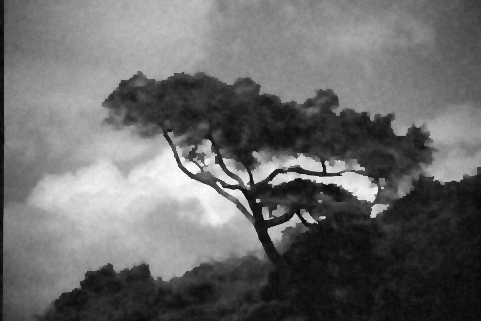
\includegraphics[scale=0.175]{pictures/denoising/image/147091_ipiano_absolute.png}
	\end{subfigure}
	\begin{subfigure}[t]{0.19\textwidth}
		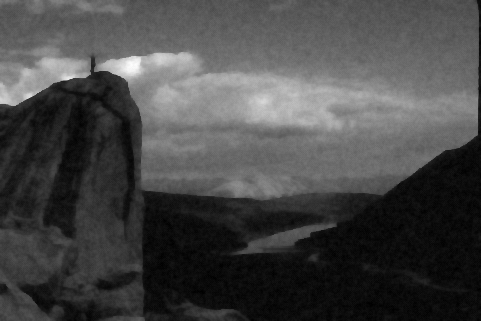
\includegraphics[scale=0.175]{pictures/denoising/image/14037_ipiano_absolute.png}
	\end{subfigure}
	\begin{subfigure}[t]{0.19\textwidth}
		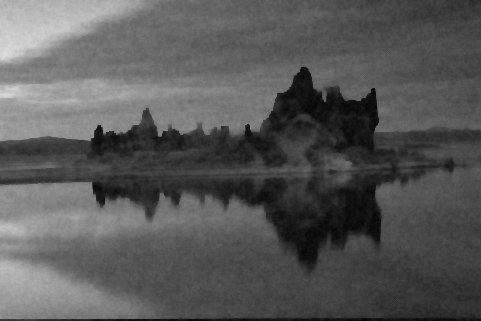
\includegraphics[scale=0.175]{pictures/denoising/image/143090_ipiano_absolute.png}
	\end{subfigure}
	\begin{subfigure}[t]{0.19\textwidth}
		
\includegraphics[scale=0.175]{pictures/denoising/image/3096_ipiano_squared.png}
	\end{subfigure}
	\begin{subfigure}[t]{0.19\textwidth}
		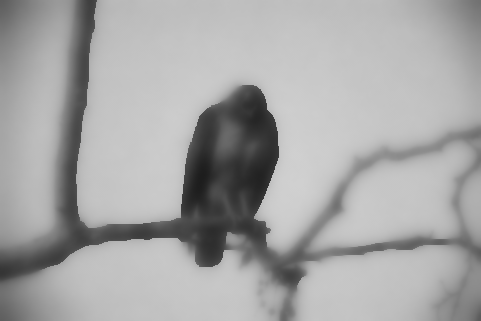
\includegraphics[scale=0.175]{pictures/denoising/image/42049_ipiano_squared.png}
	\end{subfigure}
	\begin{subfigure}[t]{0.19\textwidth}
		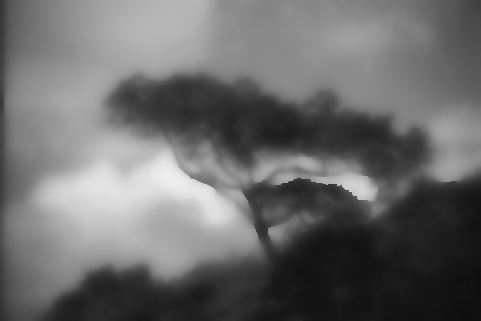
\includegraphics[scale=0.175]{pictures/denoising/image/147091_ipiano_squared.png}
	\end{subfigure}
	\begin{subfigure}[t]{0.19\textwidth}
		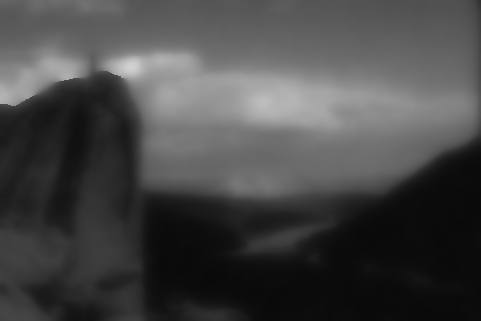
\includegraphics[scale=0.175]{pictures/denoising/image/14037_ipiano_squared.png}
	\end{subfigure}
	\begin{subfigure}[t]{0.19\textwidth}
		
\includegraphics[scale=0.175]{pictures/denoising/image/143090_ipiano_squared.png}
	\end{subfigure}
	\caption{Results of applying Algorithm \ref{alg:ipiano} to image denoising using the proposed model with the noisy image in the top row, $\rho_{1,\text{abs}}$ in the middle row and $\rho_{1,\text{sqr}}$ in the bottom row. Gaussian additive noise with standard deviation $\sigma = 0.05$ has been used. The discrete image has been scaled such that $\tilde{u}_{i,j} \in [0,1]$.}
	\label{fig:image-denoising}
\end{figure}

\subsection{Segmentation}

Following Shen \cite{Shen:2005} we want to apply Algorithm \ref{alg:ipiano} to image segmentation using a (2-)phase-field. Therefore, Shen considers the reduced Mumford-Shah\footnote{
	In particular, we consider the 2-phase model of the Mumford-Shah model.
} model \cite{MumfordShah:1989}:
\begin{align}
	h(O; c_+, c_-, u^{(0)}) = \int_{O} (u^{(0)}(x) - c_+)^2 dx + \int_{\Omega\setminus O} (u^{(0)}(x) - c_-)^2 dx + \lambda \per(O)
\end{align}
where $\lambda$ is a regularization parameter, $c_+$ and $c_-$ average intensities and $\per(O)$ is the perimeter of $O \subset \Omega$ (also called the length in \cite{Shen:2005}):
\begin{align}
	\per(O) := |\chi_O|_{BV(\Omega)},
\end{align}
\ie the total variation of the characteristics function $\chi_O$. Obviously, minimization over the set $O$ is problematic. One of the most popular approaches to this problem may be the work by Chan and Vese \cite{ChanVese:2002} who apply the level set framework. Instead, Shen -- following Ambrosio and Tortorelli \cite{AmbrosioTortorelli:1990} -- derives a $\Gamma$-convergence formulation of the reduced Mumford-Shah model:
\begin{align}
	\begin{aligned}
		h_\epsilon(u; c_+, c_-, u^{(0)}, \lambda) =& \int_{\Omega} \left(9 \epsilon \|\nabla u(x)\|_2^2 + \frac{(1 - u(x)^2)^2}{64 \epsilon}\right) dx\\
		& + \lambda \int_{\Omega}\left(\frac{1 + u(x)}{2}\right)^2(u^{(0)}(x) - c_+)^2 dx\\
		& + \lambda \int_{\Omega} \left(\frac{1 - u(x)}{2}\right)^2 (u^{(0)}(x) - c_-)^2 dx.
	\end{aligned}\label{eq:phase-field-h}
\end{align}
We briefly give the intuition behind this model without covering the necessary mathematical background. Let $u : \Omega \rightarrow [-1, 1]$ be called phase-field with the corresponding phase field energy given by
\begin{align}
	f_\epsilon(u) = \int_\Omega \left(9\epsilon \|\nabla u\|_2^2 + \frac{(1 - u^2)^2}{64 \epsilon}\right) dx.\label{eq:phase-field-f}
\end{align}
For $\epsilon > 0$ but close to $0$, this energy will force $u$ to be $1$ or $-1$ almost everywhere. Then, the perimeter $\per(O)$ can be approximated by $f_\epsilon$. In this sense Equation \eqref{eq:phase-field-f} represents an approximation to the reduced Mumford-Shah model. Shen proposes an alternating scheme to minimize $h_\epsilon$, \ie for fixed $c_+$ and $c_-$ minimize $h_\epsilon$ and for fixed $u$ compute
\begin{align}
	c_+ &= \frac{\int_\Omega (1 + u(x))^2 u^{(0)}(x) dx}{\int_\Omega (1 + u(x))^2 dx};\label{eq:segmentation-cp}\\
	c_- &= \frac{\int_\Omega (1 - u(x))^2 u^{(0)}(x) dx}{\int_\Omega (1 - u(x))^2 dx}.\label{eq:segmentation-cm}
\end{align}
As notation of Equations \eqref{eq:phase-field-h} and \eqref{eq:phase-field-f} suggests, Algorithm \ref{alg:ipiano} can be used to minimize
\begin{align}
	h_\epsilon(u; c_+, c_-, u^{(0)}, \lambda) = f_\epsilon(u) + g_{\text{sqr}}(u; c_+, c_-, u^{(0)}, \lambda)
\end{align}
with
\begin{align}
	g_{\text{sqr}}(u; c_+, c_-, u^{(0)}, \lambda) = \lambda \int_{\Omega}\left(\frac{1 + u(x)}{2}\right)^2(u^{(0)}(x) - c_+)^2 dx + \lambda \int_{\Omega} \left(\frac{1 - u(x)}{2}\right)^2 (u^{(0)}(x) - c_-)^2 dx.
\end{align}
As the integrands are continuously differentiable and $g_{\text{sqr}}$ is convex in $u$, Algorithm \ref{alg:ipiano} can easily be applied after discretization. 

Before discussing discretization and experiments, we discuss an alternative $g$ comprising absolute terms:
\begin{align}
	g_{\text{abs}}(u; c_+, c_-, u^{(0)}, \lambda) = \lambda \int_{\Omega}\frac{|1 + u(x)|}{2}(u^{(0)}(x) - c_+)^2 dx + \lambda \int_{\Omega} \frac{|1 - u(x)|}{2} (u^{(0)}(x) - c_-)dx.
\end{align}
Equations \eqref{eq:segmentation-cp} and \eqref{eq:segmentation-cm} can be adapted accordingly. As we will see, the proximal mapping needed after discretization cannot be derived using the rules presented in \cite{CombettesPesquet:2011}.

\subsubsection{Discretization}

It remains to discuss the discretization of Equation \eqref{eq:phase-field-h}. Given an image $\tilde{u}^{(0)} \in \mathbb{R}^{n \times m}$, we discretize $h_\epsilon$ as follows
\begin{align}
	f_\epsilon(\tilde{u}) &= \sum_{i = 2}^n \sum_{j = 1}^m 9 \epsilon (\tilde{u}_{i,j} - \tilde{u}_{i - 1,j})^2 + \sum_{i = 1}^n \sum_{j = 2}^m (\tilde{u}_{i,j} - \tilde{u}_{i, j - 1})^2 + \sum_{i = 1}^n \sum_{j = 1}^m \frac{1}{64 \epsilon} (1 - \tilde{u}_{i,j}^2)^2;\\
	g_{\text{sqr}}(\tilde{u}; c_+, c_-, \tilde{u}^{(0)}) &= \left[\sum_{i = 1}^n \sum_{j = 1}^m \frac{1}{4} (1 + \tilde{u}_{i,j})^2 (\tilde{u}^{(0)}_{i,j} - c_+)^2 + \sum_{i = 1}^n \sum_{j = 1}^m \frac{1}{4} (1 - \tilde{u}_{i,j})^2 (\tilde{u}^{(0)}_{i,j} - c_-)^2\right];
\end{align}
Then, $c_+$ and $c_-$ can be computed as
\begin{align}
	c_+ &= \frac{\sum_{i = 1}^n \sum_{j = 1}^m (1 + \tilde{u}_{i,j})^2 \tilde{u}^{(0)}_{i, j}}{\sum_{i = 1}^n \sum_{j = 1}^n (1 + \tilde{u}_{i,j})^2};\\
	c_- &= \frac{\sum_{i = 1}^n \sum_{j = 1}^m (1 - \tilde{u}_{i,j})^2 \tilde{u}^{(0)}_{i, j}}{\sum_{i = 1}^n \sum_{j = 1}^n (1 - \tilde{u}_{i,j})^2}.
\end{align}
Again, for $g_{\text{abs}}$ these equations can easily be adapted. Finally, the segmentation is obtained by thresholding $\tilde{u}$, \ie the foreground and background segments $S_f$, $S_b \subset \tilde{\Omega}$ are obtained as
\begin{align}
	S_f := \{(i, j) \in \tilde{\Omega} | \tilde{u}_{i,j} > \tau\},\quad S_b := \tilde{\Omega}\setminus S_f.
\end{align}

To practically implement this segmentation model using $g_{\text{abs}}$ we first rewrite the above discretization:
\begin{align}
	g_{\text{abs}}(\tilde{u}; c_+, c_-, \tilde{u}^{(0)}) &= \left[\sum_{i = 1}^n \sum_{j = 1}^m |1 + \tilde{u}_{i,j}| (\tilde{u}^{(0)}_{i,j} - c_+)^2 + |1 - \tilde{u}_{i,j}| (\tilde{u}^{(0)}_{i,j} - c_-)^2\right];
\end{align}
then, we need to derive the proximal mapping for
\begin{align}
	\rho(x) := |1 - x|C_+ + |1 + x|C_-.
\end{align}

\begin{figure}
	\centering
	\begin{subfigure}[t]{0.16\textwidth}
		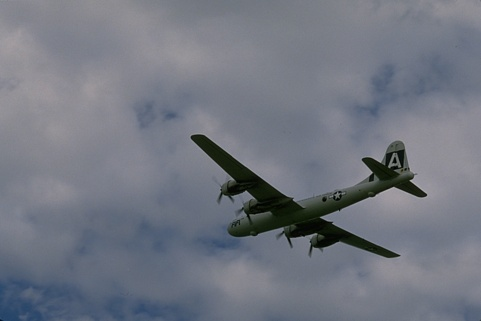
\includegraphics[scale=0.15]{pictures/3096.jpg}
	\end{subfigure}
	\begin{subfigure}[t]{0.16\textwidth}
		\includegraphics[scale=0.15]{pictures/segmentation/squared/{3096_-0.200000_seg}.png}
	\end{subfigure}
	\begin{subfigure}[t]{0.16\textwidth}
		\includegraphics[scale=0.15]{pictures/segmentation/squared/{3096_-0.100000_seg}.png}
	\end{subfigure}
	\begin{subfigure}[t]{0.16\textwidth}
		\includegraphics[scale=0.15]{pictures/segmentation/squared/{3096_0.000000_seg}.png}
	\end{subfigure}
	\begin{subfigure}[t]{0.16\textwidth}
		\includegraphics[scale=0.15]{pictures/segmentation/squared/{3096_0.100000_seg}.png}
	\end{subfigure}
	\begin{subfigure}[t]{0.16\textwidth}
		\includegraphics[scale=0.15]{pictures/segmentation/squared/{3096_0.200000_seg}.png}
	\end{subfigure}
	\vskip 2px
	%%%%%%%%%%%%%%%%%%%%%%%%%%%%%%%%
	\begin{subfigure}[t]{0.16\textwidth}
		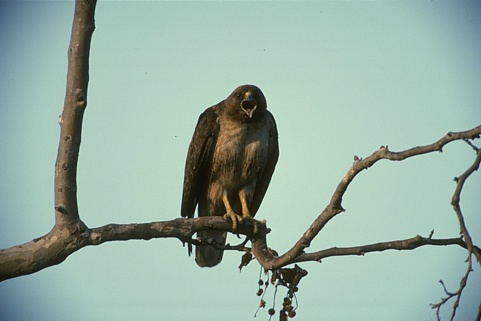
\includegraphics[scale=0.15]{pictures/42049.jpg}
	\end{subfigure}
	\begin{subfigure}[t]{0.16\textwidth}
		\includegraphics[scale=0.15]{pictures/segmentation/squared/{42049_-0.200000_seg}.png}
	\end{subfigure}
	\begin{subfigure}[t]{0.16\textwidth}
		\includegraphics[scale=0.15]{pictures/segmentation/squared/{42049_-0.100000_seg}.png}
	\end{subfigure}
	\begin{subfigure}[t]{0.16\textwidth}
		\includegraphics[scale=0.15]{pictures/segmentation/squared/{42049_0.000000_seg}.png}
	\end{subfigure}
	\begin{subfigure}[t]{0.16\textwidth}
		\includegraphics[scale=0.15]{pictures/segmentation/squared/{42049_0.100000_seg}.png}
	\end{subfigure}
	\begin{subfigure}[t]{0.16\textwidth}
		\includegraphics[scale=0.15]{pictures/segmentation/squared/{42049_0.200000_seg}.png}
	\end{subfigure}
	\vskip 2px
	%%%%%%%%%%%%%%%%%%%%%%%%%%%%%%%%
	\begin{subfigure}[t]{0.16\textwidth}
		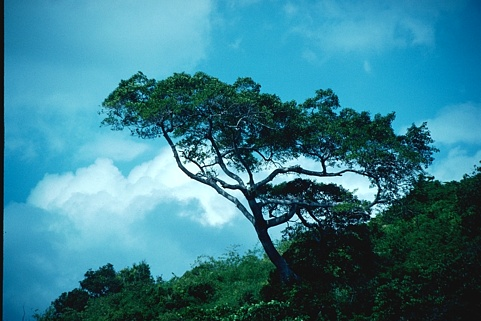
\includegraphics[scale=0.15]{pictures/147091.jpg}
	\end{subfigure}
	\begin{subfigure}[t]{0.16\textwidth}
		\includegraphics[scale=0.15]{pictures/segmentation/squared/{147091_-0.200000_seg}.png}
	\end{subfigure}
	\begin{subfigure}[t]{0.16\textwidth}
		\includegraphics[scale=0.15]{pictures/segmentation/squared/{147091_-0.100000_seg}.png}
	\end{subfigure}
	\begin{subfigure}[t]{0.16\textwidth}
		\includegraphics[scale=0.15]{pictures/segmentation/squared/{147091_0.000000_seg}.png}
	\end{subfigure}
	\begin{subfigure}[t]{0.16\textwidth}
		\includegraphics[scale=0.15]{pictures/segmentation/squared/{147091_0.100000_seg}.png}
	\end{subfigure}
	\begin{subfigure}[t]{0.16\textwidth}
		\includegraphics[scale=0.15]{pictures/segmentation/squared/{147091_0.200000_seg}.png}
	\end{subfigure}
	\vskip 2px
	%%%%%%%%%%%%%%%%%%%%%%%%%%%%%%%%
	\begin{subfigure}[t]{0.16\textwidth}
		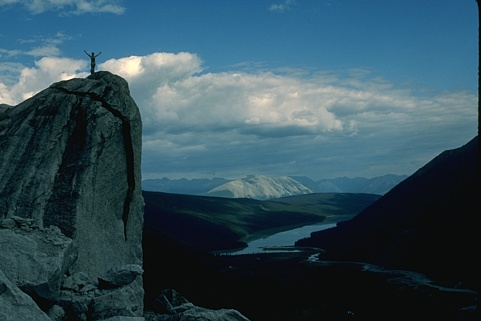
\includegraphics[scale=0.15]{pictures/14037.jpg}
	\end{subfigure}
	\begin{subfigure}[t]{0.16\textwidth}
		\includegraphics[scale=0.15]{pictures/segmentation/squared//{14037_-0.200000_seg}.png}
	\end{subfigure}
	\begin{subfigure}[t]{0.16\textwidth}
		\includegraphics[scale=0.15]{pictures/segmentation/squared/{14037_-0.100000_seg}.png}
	\end{subfigure}
	\begin{subfigure}[t]{0.16\textwidth}
		\includegraphics[scale=0.15]{pictures/segmentation/squared/{14037_0.000000_seg}.png}
	\end{subfigure}
	\begin{subfigure}[t]{0.16\textwidth}
		\includegraphics[scale=0.15]{pictures/segmentation/squared/{14037_0.100000_seg}.png}
	\end{subfigure}
	\begin{subfigure}[t]{0.16\textwidth}
		\includegraphics[scale=0.15]{pictures/segmentation/squared/{14037_0.200000_seg}.png}
	\end{subfigure}
	\vskip 2px
	%%%%%%%%%%%%%%%%%%%%%%%%%%%%%%%%
	\begin{subfigure}[t]{0.16\textwidth}
		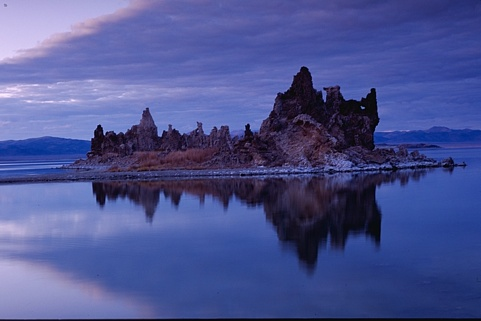
\includegraphics[scale=0.15]{pictures/143090.jpg}
	\end{subfigure}
	\begin{subfigure}[t]{0.16\textwidth}
		\includegraphics[scale=0.15]{pictures/segmentation/squared/{143090_-0.200000_seg}.png}
	\end{subfigure}
	\begin{subfigure}[t]{0.16\textwidth}
		\includegraphics[scale=0.15]{pictures/segmentation/squared/{143090_-0.100000_seg}.png}
	\end{subfigure}
	\begin{subfigure}[t]{0.16\textwidth}
		\includegraphics[scale=0.15]{pictures/segmentation/squared/{143090_0.000000_seg}.png}
	\end{subfigure}
	\begin{subfigure}[t]{0.16\textwidth}
		\includegraphics[scale=0.15]{pictures/segmentation/squared/{143090_0.100000_seg}.png}
	\end{subfigure}
	\begin{subfigure}[t]{0.16\textwidth}
		\includegraphics[scale=0.15]{pictures/segmentation/squared/{143090_0.200000_seg}.png}
	\end{subfigure}
	\caption{Segmentation results for five images from the Berkeley Segmentation Dataset \cite{ArbelaezMaireFowlkesMalik:2011} for thresholds $\tau = -0.1, -0.2, 0.0, 0.1, 0.2$ and using $g_{\text{sqr}}$; the foreground segment $S_f$ is depicted in white.}
	\label{fig:segmentation}
\end{figure}

\begin{lemmamd}
	For $\rho$ as defined above, the proximal mapping $\prox{\alpha \rho}$ is given as
	\begin{align}
		\prox{\alpha \rho}(x) = \begin{cases}
			- \alpha(C_+ + C_-) + x&\quad x > 1 + \alpha(C_+ + C_-)\\
			1&\quad x \in [1 + \alpha(C_+ - C_-), 1 + \alpha(C_p + C_-)\\
			\alpha(-C_+ + C_-) + x&\quad x \in (-1 + \alpha(C_+ - C_-), 1 + \alpha(C_+ - C_-))\\
			-1&\quad x \in [ -1 - \alpha(C_+ + C_-), -1 + \alpha(C_+ - C_-)]\\
			\alpha(C_+ + C_-) + x&\quad x < -1 - \alpha(C_+ + C_-)
		\end{cases}.\label{eq:prox-segmentation}
	\end{align}
\end{lemmamd}

\begin{proof}
	We first rewrite $\rho$ as piecewise linear function:
	\begin{align}
		\rho(x) = |1 - x|C_- + |1 - x|C_+.
	\end{align}
	The proximal mapping is then defined as
	\begin{align}
		\prox{\alpha \rho}(x) = \argmin_{\hat{x}}\alpha \rho(\hat{x}) + \frac{1}{2}(\hat{x} - x)^2.
	\end{align}
	Note that without loss of generality we can assume $\alpha = 1$ as $\alpha$ merely scales $C_+$ and $C_-$. Then, using the subdifferential
	\begin{align}
		\partial \rho(x) = \begin{cases}
			C_+ + C_-&\quad x > 1\\
			[C_+ - C_-, C_+ + C_-]&\quad x = 1\\
			C_+ - C_-&\quad -1 < x < 1\\
			[-(C_+ + C_-), C_+ - C_-]&\quad x = -1\\
			-(C_+ + C_-)&\quad x < -1
		\end{cases},
	\end{align}
	we derive the first-order condition
	\begin{align}
		\partial \rho(\hat {x}) + (\hat{x} - x).
	\end{align}
	We distinguish the following cases:
	\setlist[enumerate,1]{leftmargin=0.75cm}
	\begin{enumerate}[label=\arabic*)]
		\item $x > 1$ gives
		\begin{align}
			C_+ + C_- + \hat{x} - x = 0\quad&\Leftrightarrow\quad \hat {x} = -(C_+ + C_-) + x\\
			&\Rightarrow \hat{x} > 1 \quad\Leftrightarrow\quad x > 1 + C_+ + C_-
		\end{align}
		\item $-1 < x < 1$ gives
		\begin{align}
			C_+ - C_- + \hat{x} - x = 0 \quad&\Leftrightarrow\quad \hat {x} = - C_+ + C_- + x\\
			&\Rightarrow -1 < \hat{x} < 1 \quad\Leftrightarrow\quad -1 + C_+ - C_- < x < 1 + C_+ - C_-.
		\end{align}
		\item $x < -1$ gives
		\begin{align}
			-(C_+ + C_-) + \hat{x} - x = 0 \quad&\Leftrightarrow\quad \hat{x} = (C_+ + C_-) + x\\
			&\Rightarrow \hat{x} < -1 \quad\Leftrightarrow\quad x < -1 - (C_+ + C_-).
		\end{align}
	\end{enumerate}
	It remains to discuss the following cases:
	\setlist[enumerate,1]{leftmargin=0.75cm}
	\begin{enumerate}[label=\arabic*)]
		\setcounter{enumi}{3}
		\item $x = 1 + C_+ + C_-$ and $x = 1 + C_+ - C_-$ give $\hat{x} = 1$.
		\item $x = -1 + C_+ - C_-$ and $x = -1 - (C_+ + C_-)$ give $\hat{x} = -1$.
	\end{enumerate}
	Overall, Equation \eqref{eq:prox-segmentation} follows.
\end{proof}

\subsubsection{Experiments}

We conducted experiments on several color images from the Berkeley Segmentation Dataset \cite{ArbelaezMaireFowlkesMalik:2011}; results for several thresholds $\tau$ and $\lambda = 100$ using $g_{\text{sqr}}$ are shown in Figure \ref{fig:segmentation}. Figure \ref{fig:segmentation-absolute}, in contrast, shows results using $g_{\text{abs}}$. As can be seen, using $g_{\text{abs}}$ resolves parts of the artifacts on the lower left border of the ``airplane' image. However, this also removes clear contours around the airplane.

\begin{figure}
	\centering
	\begin{subfigure}[t]{0.16\textwidth}
		\includegraphics[scale=0.15]{pictures/3096.jpg}
	\end{subfigure}
	\begin{subfigure}[t]{0.16\textwidth}
		\includegraphics[scale=0.15]{pictures/segmentation/absolute/{3096_-0.200000_seg}.png}
	\end{subfigure}
	\begin{subfigure}[t]{0.16\textwidth}
		\includegraphics[scale=0.15]{pictures/segmentation/absolute/{3096_-0.100000_seg}.png}
	\end{subfigure}
	\begin{subfigure}[t]{0.16\textwidth}
		\includegraphics[scale=0.15]{pictures/segmentation/absolute/{3096_0.000000_seg}.png}
	\end{subfigure}
	\begin{subfigure}[t]{0.16\textwidth}
		\includegraphics[scale=0.15]{pictures/segmentation/absolute/{3096_0.100000_seg}.png}
	\end{subfigure}
	\begin{subfigure}[t]{0.16\textwidth}
		\includegraphics[scale=0.15]{pictures/segmentation/absolute/{3096_0.200000_seg}.png}
	\end{subfigure}
	\caption{Segmentation results for an image from the Berkeley Segmentation Dataset \cite{ArbelaezMaireFowlkesMalik:2011} for thresholds $\tau = -0.2, -0.1, 0.0, 0.1, 0.2$ and using $g_{\text{abs}}$; the foreground segment $S_f$ is depicted in white.}
	\label{fig:segmentation-absolute}
\end{figure}

%\subsection{Future Work}

%We would like to extend the presented approximation to the reduced Mumford-Shah model using an absolute distance $|1 \rpm u(x)|$ as weighting in Equation \eqref{eq:phase-field-h}. However, we were not able to implement and minimize the corresponding proximal mapping.

\section{Conclusion}
\label{sec:conclusion}

In this paper, we introduced the iPiano algorithm for minimization of non-convex and non-smooth composite functions. Following Ochs \etal \cite{OchsChenBroxPock:2013}, we proved convergence for objectives satisfying the Kurdyka-Lojasiewicz property \cite{Lojasiewicz:1993,Kurdyka:1998} and discussed the practical implementation of the proposed algorithm. Finally, we discussed the application of iPiano to image denoising and image segmentation. Overall, we showed that iPiano is able to reliably minimize non-smooth and non-convex composite functions frequently used in image processing and computer vision applications.

\subsection{Connection to \cite{Berkels:2015}}

In \cite[Bem. 4.12]{Berkels:2015}, Berkels introduces the reader to the forward-backward splitting algorithm where iterates are computed according to
\begin{align}
	x^{(n + 1)} = \prox{\alpha g}(x^{(n)} - \nabla f(x^{(n)})),\label{eq:fb-iteration}
\end{align}
assuimg that both $g$ and $f$ are proper closed convex and $f$ is continuously differentiable. As mentioned in Section \ref{sec:related-work}, Ochs \etal extend this scheme by adding an inertial force (\ie a momentum term) and disregarding the requirement of $f$ being proper closed convex. In particular, Equation \eqref{eq:iteration} extends Equation \eqref{eq:fb-iteration} by the inertial force term $\beta_n(x^{(n)} - x^{(n - 1)})$.

\bibliographystyle{siamplain}
\bibliography{paper}

\begin{appendix}
	\section{C++ Implementation}
	
	The following sections present a C++ implementation of Algorithms \ref{alg:nmipiano} and \ref{alg:ipiano}. The implementation requires C++11, OpenCV, Eigen as well as Google GLOG and will be made publicly available at \url{https://github.com/davidstutz}. For brevity, some details are skipped in the following listings.
	
	\subsection{nmiPiano}
	
	The following listing presents the implementation of Algorithm \ref{alg:nmipiano}, \ie nmiPiano.
	
	\vspace{-0.3cm}
	\begin{lstlisting}
#ifndef NMIPIANO_H
#define	NMIPIANO_H

#include <random>
#include <fstream>
#include <functional>
#include <Eigen/Dense>
#include <glog/logging.h>

/** \brief Implementation of nmiPiano (algorithm 4) as proposed in [1]:
 *  [1] P. Ochs, Y. Chen, T. Brox, T. Pock.
 *      iPiano: Inertial Proximal Algorithm for Nonconvex Optimization.
 *      SIAM J. Imaging Sciences, vol. 7, no. 2, 2014.
 * \author David Stutz
 */
class nmiPiano
{
public:
    
    /** \brief Options of algorithm. */
    struct Options
    {
        /** \brief Initial iterate. */
        Eigen::MatrixXf x_0;
        /** \brief Maximum number of iterations. */
        unsigned int max_iter;
        /** \brief Fixed beta in [0, 1). */
        float beta = 0.5f;
        /** \brief Fixed eta for backtracking the local lipschitz constant. */
        float eta = 1.05f;
        /** \brief Initialization of loca Lipschitz. */
        float L_0m1 = 1.f;
        /** \brief Whether to bound estimated Lipschitz constant below by the given L_n. */
        bool BOUND_L_N = false;
        /** \brief Termination criterion; stop if Delta_n smaller than epsilon. */
        float epsilon = 0;
    };
    
    /** \brief Structure representing an iteration, passed as is to a callback function
     * to be able to monitor process. */
    struct Iteration
    {
        /** \brief Current iterate. */
        Eigen::MatrixXf x_n;
        /** \brief Last iterate. */
        Eigen::MatrixXf x_nm1;
        /** \brief Update: x_np1 = x_n + Delta_x_n. */
        Eigen::MatrixXf Delta_x_n;
        /** \brief Difference between two iterates. */
        float Delta_n;
        /** \brief Smooth objective function at current iterate. */
        float f_x_n;
        /** \brief Derivative of smooth objective at current iterate. */
        Eigen::MatrixXf df_x_n;
        /** Nonsmooth objective function at current iterate. */
        float g_x_n;
        /** \brief L_n of current iterate (within iterations, this is also used to estimate L_np1 via backtracking). */
        float L_n;
        /** \brief alpha_n of current iterate (within iterations, this is also used to estimate alpha_np1). */
        float alpha_n;
        /** \brief Current iteration. */
        int n;
    };
    
    // Definition of different callbacks skipped ...
    
    /** \brief Constructor.
     * \param[in] f
     * \param[in] df
     * \param[in] prox_g
     * \param[in] callback
     */
    nmiPiano(const std::function<float(const Eigen::MatrixXf&)> f, 
            const std::function<void(const Eigen::MatrixXf&, Eigen::MatrixXf&)> df,
            std::function<float(const Eigen::MatrixXf&)> g,
            const std::function<void(const Eigen::MatrixXf&, Eigen::MatrixXf&, float alpha)> prox_g,
            Options options,
            const std::function<void(const Iteration&)> callback = [](const Iteration &iteration) -> void { /* Nothing ... */ });
            
    /** \brief Destructor. */
    ~nmiPiano();
    
    /** \brief Optimize the given objective using the nmiPiano algorithm. 
     * \param[out] x_star
     * \param[out] f_x_star
     */
    void optimize(Eigen::MatrixXf &x_star, float &f_x_star);
    
protected:
    
    /** \brief Initialize the iteration structure (i.e. set iteration 0): 
     * \param[in] iteration
     */
    void initialize(Iteration &iteration);
    
    float estimateL(const Iteration &iteration);
    
    /** \brief Do an iteration, i.e. compute x_np1.
     * \param[in] iteration
     * \param[in] beta
     * \param[out] x_np1
     */
    void iterate(Iteration &iteration, float beta, Eigen::MatrixXf &x_np1);
    
    /** \brief Check the lipschitz condition for backtracking.
     * \param[in] iteration
     * \param[in] x_np1
     * \return
     */
    bool checkLipschitz(const Iteration& iteration, const Eigen::MatrixXf &x_np1);
    
    /** \brief The smooth part of the objective function. */
    std::function<float(const Eigen::MatrixXf&)> f_;
    /** \brief Gradient of smooth part of the objective function (i.e. derivative). */
    std::function<void(const Eigen::MatrixXf&, Eigen::MatrixXf&)> df_;
    /** \brief Convex, nonsmooth part of objective. */
    std::function<float(const Eigen::MatrixXf&)> g_;
    /** \brief Proximal map for g, i.e. (I + alpha_n*g)^(-1). */
    std::function<void(const Eigen::MatrixXf&, Eigen::MatrixXf&, float)> prox_g_;
    /** \brief Callback, can e.g. be sued to monitor process using the provided information in the Iteration structure. */
    std::function<void(const Iteration&)> callback_;
    /** \brief Options.*/
    Options options_;
};

// Implementation of different callbacks skipped ...

////////////////////////////////////////////////////////////////////////////////
// nmiPiano::nmiPiano
////////////////////////////////////////////////////////////////////////////////

nmiPiano::nmiPiano(const std::function<float(const Eigen::MatrixXf&)> f, 
        const std::function<void(const Eigen::MatrixXf&,Eigen::MatrixXf&)> df, 
        std::function<float(const Eigen::MatrixXf &)> g,
        const std::function<void(const Eigen::MatrixXf&, Eigen::MatrixXf&, float alpha)> prox_g,
        nmiPiano::Options options,
        const std::function<void(const nmiPiano::Iteration&)> callback)
{
    f_ = f;
    df_ = df;
    g_ = g;
    prox_g_ = prox_g;
    callback_ = callback;
    options_ = options;
}

////////////////////////////////////////////////////////////////////////////////
// nmiPiano::~nmiPiano
////////////////////////////////////////////////////////////////////////////////

nmiPiano::~nmiPiano()
{
    // ...
}

////////////////////////////////////////////////////////////////////////////////
// nmiPiano::optimize
////////////////////////////////////////////////////////////////////////////////

void nmiPiano::optimize(Eigen::MatrixXf &x_star, float &f_x_star)
{
    nmiPiano::Iteration iteration;
    initialize(iteration);
    
    // Used for backtracking; referring to the next iterate x_np1:
    Eigen::MatrixXf x_np1;
    
    for (unsigned int t = 0; t <= options_.max_iter; t++)
    {
        callback_(iteration);
        
        // Backtrack for the lipschitz constant L_n:
        float L_nm1 = estimateL(iteration);
        
        // Fall back to last L_n in worst case.
        if (std::isinf(L_nm1) || std::isnan(L_nm1) || options_.BOUND_L_N)
        {
            LOG_IF(INFO, !options_.BOUND_L_N) << "Could not get starting value for local Lipschitz constant, using L_nm1 instead (L_n = " << L_nm1 << ")";
            L_nm1 = iteration.L_n;
        }
        
        bool condition = false;
        
        int l = 0; // Backtracking steps.
        do
        {
            iteration.L_n = std::pow(options_.eta,  l)*L_nm1;
            
            LOG_IF(FATAL, std::isinf(iteration.L_n) || std::isnan(iteration.L_n)) 
                    << "Could not find the local Lipschitz constant - L_n = " 
                    << iteration.L_n << std::endl;
            LOG_IF(INFO, l > 0 && l%1000 == 0) 
                    << "Having a hard time finding the local Lipschitz constant (L_n = " << iteration.L_n 
                    << "; L_nm1 = " << L_nm1 << "; eta = " << options_.eta << "; l = " << l << ")" << std::endl;
            
            iteration.alpha_n = 2*(1 - options_.beta)/iteration.L_n;
            LOG_IF(FATAL, iteration.alpha_n < 0)
                    << "Cannot choose alpha_n - it does not exist: alpha_n = " 
                    << iteration.alpha_n << " (L_n = " << iteration.L_n << ")!";
            
            
            // We fixes L_n and alpha_n, so we can try an iteration to check the
            // Lipschitz condition.
            iterate(iteration, options_.beta, x_np1);
            condition = checkLipschitz(iteration, x_np1);
            
            l++;
        }
        while (!condition); // Now alpha_n and L_n are set correctly.
        
        iteration.x_nm1 = iteration.x_n;
        iteration.x_n = x_np1;
        
        // For iteration 0, this is done in initialize():
        iteration.f_x_n = f_(iteration.x_n);
        iteration.g_x_n = g_(iteration.x_n);
        df_(iteration.x_n, iteration.df_x_n);
        
        LOG_IF(FATAL, iteration.x_n.rows() != iteration.df_x_n.rows() 
                || iteration.x_n.cols() != iteration.df_x_n.cols()) << "Output dimensions of df invalid.";
        
        iteration.n++;
        
        // Termination criterion
        if (iteration.Delta_n < options_.epsilon && options_.epsilon > 0)
        {
            break;
        }
    }
    
    x_star = iteration.x_n;
    f_x_star = iteration.f_x_n;
}

////////////////////////////////////////////////////////////////////////////////
// nmiPiano::initialize
////////////////////////////////////////////////////////////////////////////////

void nmiPiano::initialize(nmiPiano::Iteration &iteration)
{
    iteration.n = 0;
    iteration.x_n = options_.x_0;
    iteration.x_nm1 = options_.x_0;
    
    iteration.g_x_n = g_(iteration.x_n);
    iteration.f_x_n = f_(iteration.x_n);
    df_(iteration.x_n, iteration.df_x_n);
    
    LOG_IF(FATAL, iteration.x_n.rows() != iteration.df_x_n.rows() 
            || iteration.x_n.cols() != iteration.df_x_n.cols()) << "Output dimensions of df invalid.";
    
    iteration.alpha_n = 0.1f; // Required for estimateL!
    
    // Estimate L_n.
    if (options_.L_0m1 > 0)
    {
        iteration.L_n = options_.L_0m1;
    }
    
    // Estimate L and take max.
    if (iteration.df_x_n.squaredNorm() > 0.001)
    {
        iteration.L_n = std::max(iteration.L_n, estimateL(iteration));
    }
    
    iteration.alpha_n = 2*(1 - options_.beta)/iteration.L_n;
}

float nmiPiano::estimateL(const nmiPiano::Iteration &iteration)
{
    Eigen::MatrixXf x_tilde = iteration.x_n - iteration.alpha_n*iteration.df_x_n;

    Eigen::MatrixXf df_x_tilde;
    df_(x_tilde, df_x_tilde);

    Eigen::MatrixXf delta_df_x = iteration.df_x_n - df_x_tilde;
    Eigen::MatrixXf delta_x = iteration.x_n - x_tilde;
    
    float L_n = std::sqrt(delta_df_x.squaredNorm())/std::sqrt(delta_x.squaredNorm ());
    if (options_.BOUND_L_N) {
        L_n = std::max(L_n, options_.L_0m1);
    }
    
    return L_n;
}

////////////////////////////////////////////////////////////////////////////////
// nmiPiano::iterate
////////////////////////////////////////////////////////////////////////////////

void nmiPiano::iterate(nmiPiano::Iteration& iteration, float beta, Eigen::MatrixXf& x_np1)
{
    // TODO: precompute x_n - x_nm1
    iteration.Delta_x_n = - iteration.alpha_n*iteration.df_x_n + beta*(iteration.x_n - iteration.x_nm1);
    
    prox_g_(iteration.x_n + iteration.Delta_x_n, x_np1, iteration.alpha_n);
    
    LOG_IF(FATAL, iteration.x_n.rows() != x_np1.rows() 
            || iteration.x_n.cols() != x_np1.cols()) << "Output dimensions of prox_g invalid.";
    
    Eigen::MatrixXf Delta_n = iteration.x_n - x_np1;
    iteration.Delta_n = std::sqrt(Delta_n.squaredNorm());
}

////////////////////////////////////////////////////////////////////////////////
// nmiPiano::checkLipschitz
////////////////////////////////////////////////////////////////////////////////

bool nmiPiano::checkLipschitz(const nmiPiano::Iteration& iteration, const Eigen::MatrixXf& x_np1)
{
    float f_x_np1 = f_(x_np1);
    
    Eigen::MatrixXf residual = x_np1 - iteration.x_n;
    Eigen::MatrixXf product = iteration.df_x_n.array()*residual.array();
    float threshold = iteration.f_x_n + product.squaredNorm() + iteration.L_n/2.f * residual.squaredNorm();
    
    return (f_x_np1 <= threshold);
}

#endif	/* NMIPIANO_H */
	\end{lstlisting}
	
	\subsection{iPiano}
	
	The following listing presents the implementation of Algorithm \ref{alg:ipiano}, \ie iPiano.
	
	\vspace{-0.3cm}
	\begin{lstlisting}
#ifndef IPIANO_H
#define	IPIANO_H

#include <random>
#include <fstream>
#include <functional>
#include <Eigen/Dense>
#include <glog/logging.h>

#include "nmipiano.h"

/** \brief Implementation of iPiano (algorithm 5) as proposed in [1]:
 *  [1] P. Ochs, Y. Chen, T. Brox, T. Pock.
 *      iPiano: Inertial Proximal Algorithm for Nonconvex Optimization.
 *      SIAM J. Imaging Sciences, vol. 7, no. 2, 2014.
 * \author David Stutz
 */
class iPiano : public nmiPiano
{
public:
    
    /** \brief Options of algorithm. */
    struct Options : public nmiPiano::Options
    {
        /** \brief beta_0m1 to initialize alpha_0m1, delta_0m1 and gamma_0m1 according to Equations (21) and (22). */
        float beta_0m1 = 0.5f;
        /** \brief Fixed c_1. */
        float c_1 = 1e-8;
        /** \brief Fixed c_2. */
        float c_2 = 1e-8;
        /** \brief Number of dicsrete steps for alpha_n and beta_n to try. */
        int steps = 10000;
    };
    
    /** \brief Structure representing an iteration, passed as is to a callback function
     * to be able to monitor process. */
    struct Iteration : public nmiPiano::Iteration
    {
        /** \brief beta_n of current iterate (within iterations, this is also used to estimate beta_np1). */
        float beta_n;
        /** \brief delta_n of current iterate (within iterations, this is also used to estimate delta_np1). */
        float delta_n;
        /** \brief gamma_n of current iterate (within iterations, this is also used to estimate gamma_np1). */
        float gamma_n;
    };
    
    // Definition of different callbacks skipped ...
    
    /** \brief Constructor.
     * \param[in] f
     * \param[in] df
     * \param[in] prox_g
     * \param[in] callback
     */
    iPiano(const std::function<float(const Eigen::MatrixXf&)> f, 
            const std::function<void(const Eigen::MatrixXf&, Eigen::MatrixXf&)> df,
            std::function<float(const Eigen::MatrixXf&)> g,
            const std::function<void(const Eigen::MatrixXf&, Eigen::MatrixXf&, float alpha)> prox_g,
            Options options,
            const std::function<void(const Iteration&)> callback = [](const Iteration &iteration) -> void { /* Nothing ... */ });
            
    /** \brief Destructor. */
    ~iPiano();
    
    /** \brief Optimize the given objective using the iPiano algorithm. 
     * \param[out] x_star
     * \param[out] f_x_star
     */
    void optimize(Eigen::MatrixXf &x_star, float &f_x_star);
    
protected:
    
    /** \brief Initialize the iteration structure (i.e. set iteration 0): 
     * \param[in] iteration
     */
    void initialize(Iteration &iteration);
    
    /** \brief Callback, note: overwrites nmiPiano::callback_! */
    std::function<void(const Iteration&)> callback_;
    /** \brief Options (note: overwrites nmiPiano::options_!). */
    Options options_;
};

// Implementation of different callbacks skipped ...

////////////////////////////////////////////////////////////////////////////////
// iPiano::iPiano
////////////////////////////////////////////////////////////////////////////////

iPiano::iPiano(const std::function<float(const Eigen::MatrixXf&)> f, 
        const std::function<void(const Eigen::MatrixXf&,Eigen::MatrixXf&)> df, 
        std::function<float(const Eigen::MatrixXf &)> g,
        const std::function<void(const Eigen::MatrixXf&, Eigen::MatrixXf&, float alpha)> prox_g,
        iPiano::Options options,
        const std::function<void(const iPiano::Iteration&)> callback)
        : nmiPiano(f, df, g, prox_g, options)
{
    options_ = options;
    callback_ = callback;
}

////////////////////////////////////////////////////////////////////////////////
// iPiano::~iPiano
////////////////////////////////////////////////////////////////////////////////

iPiano::~iPiano()
{
    // ...
}

////////////////////////////////////////////////////////////////////////////////
// iPiano::optimize
////////////////////////////////////////////////////////////////////////////////

void iPiano::optimize(Eigen::MatrixXf &x_star, float &f_x_star)
{
    iPiano::Iteration iteration;
    initialize(iteration);
    
    // Used for backtracking; referring to the next iterate x_np1:
    Eigen::MatrixXf x_np1;
    
    for (unsigned int t = 0; t <= options_.max_iter; t++)
    {
        callback_(iteration);
        
        // Backtrack for the Lipschitz constant L_n and the updates
        // alpha_n and beta_n:
        float L_nm1 = estimateL(iteration);
        
        // Fall back to last L_n in worst case.
        if (std::isinf(L_nm1) || std::isnan(L_nm1) || options_.BOUND_L_N)
        {
            LOG_IF(INFO, !options_.BOUND_L_N) << "Could not get starting value for local Lipschitz constant, using L_nm1 (L_n = " << L_nm1 << ")";
            L_nm1 = iteration.L_n;
        }
        
        float delta_nm1 = iteration.delta_n;
        bool condition = false;
        
        int l = 0;
        do
        {
            iteration.L_n = std::pow(options_.eta, l)*L_nm1;
            
            LOG_IF(FATAL, std::isinf(iteration.L_n) || std::isnan(iteration.L_n)) 
                    << "Could not find the local Lipschitz constant - L_n = " 
                    << iteration.L_n << std::endl;
            LOG_IF(INFO, l > 0 && l%1000 == 0) 
                    << "Having a hard time finding the local Lipschitz constant (L_n = " << iteration.L_n 
                    << "; L_nm1 = " << L_nm1 << "; eta = " << options_.eta << "; l = " << l << ")" << std::endl;
            
            float b = (delta_nm1 + iteration.L_n/2)/(options_.c_2 + iteration.L_n/2);
            float beta = (b - 1)/(b - 1.f/2.f);
//            float beta = 0.999;
            
            for (iteration.beta_n = beta; iteration.beta_n >= 0; 
                    iteration.beta_n -= beta/options_.steps)
            {
                bool take = false; // Whether to take current beta_n.
//                float alpha = 2*(1 - iteration.beta_n)/(iteration.L_n/2.f + options_.c_2);
                float alpha = 2*(1 - iteration.beta_n)/(iteration.L_n);
                
                LOG_IF(FATAL, alpha < options_.c_1)
                        << "Cannot choose alpha_n - it does not exist: c_1 = " 
                        << options_.c_1  << "; alpha_n = " << alpha
                        << " (L_n = " << iteration.L_n << ")!";
                
                for (iteration.alpha_n = alpha; iteration.alpha_n > options_.c_1; 
                        iteration.alpha_n -= (alpha - options_.c_1)/options_.steps)
                {
                    // TODO save some computation here!
                    iteration.delta_n = 1/iteration.alpha_n - iteration.L_n/2 
                            - iteration.beta_n/(2*iteration.alpha_n);
                    iteration.gamma_n = 1/iteration.alpha_n - iteration.L_n/2 
                            - iteration.beta_n/iteration.alpha_n;
                    
                    if (iteration.delta_n < delta_nm1
                            && iteration.delta_n >= iteration.gamma_n 
                            && iteration.gamma_n >= options_.c_2)
                    {
                        // Good parameters, so take these!
                        take = true;
                        break;
                    }
                }
                
                if (take)
                {
                    break;
                }
            }
                
            // We fixes L_n and alpha_n, so we can try an iteration to check the
            // Lipschitz condition.
            iterate(iteration, iteration.beta_n, x_np1);
            condition = checkLipschitz(iteration, x_np1);
            
            l++;
        }
        while (!condition); // Now alpha_n and L_n are set correctly.
        
        iteration.x_nm1 = iteration.x_n;
        iteration.x_n = x_np1;
        
        // For iteration 0, this is done in initialize():
        iteration.f_x_n = f_(iteration.x_n);
        iteration.g_x_n = g_(iteration.x_n);
        df_(iteration.x_n, iteration.df_x_n);
        
        LOG_IF(FATAL, iteration.x_n.rows() != iteration.df_x_n.rows() 
                || iteration.x_n.cols() != iteration.df_x_n.cols()) << "Output dimensions of df invalid.";
       
        iteration.n++;
        
        // Termination criterion
        if (iteration.Delta_n < options_.epsilon && options_.epsilon > 0)
        {
            break;
        }
    }
    
    x_star = iteration.x_n;
    f_x_star = iteration.f_x_n;
}

////////////////////////////////////////////////////////////////////////////////
// iPiano::initialize
////////////////////////////////////////////////////////////////////////////////

void iPiano::initialize(iPiano::Iteration &iteration)
{
    iteration.n = 0;
    iteration.x_n = options_.x_0;
    iteration.x_nm1 = options_.x_0;
    
    iteration.g_x_n = g_(iteration.x_n);
    iteration.f_x_n = f_(iteration.x_n);
    
    df_(iteration.x_n, iteration.df_x_n);
    
    LOG_IF(FATAL, iteration.x_n.rows() != iteration.df_x_n.rows() 
            || iteration.x_n.cols() != iteration.df_x_n.cols()) << "Output dimensions of df invalid.";
    
    iteration.alpha_n = 0.1f; // Required for estimateL!
    
    // Estimate L_n.
    if (options_.L_0m1 > 0)
    {
        iteration.L_n = options_.L_0m1;
    }
    
    // Estimate L and take max.
    if (iteration.df_x_n.squaredNorm() > 0.001)
    {
        iteration.L_n = std::max(iteration.L_n, estimateL(iteration));
    }
    
    // beta_0m1 is given by the options!
    iteration.beta_n = options_.beta_0m1;
    
    // Initialize alpha_0m1 to suffice alpha_0m1 <= 2*(1 - beta_0m)/L_0m1
    // and delta_0m1 >= gamma_0m1 > c_2 where delta_0m1 and gamma_0m1 depend upon alpha_0m1.
    
//    float alpha = 2*(1 - iteration.beta_n)/(iteration.L_n/2.f + options_.c_2);
    float alpha = 2*(1 - iteration.beta_n)/(iteration.L_n);
    
    LOG_IF(FATAL, alpha < options_.c_1)
            << "Cannot choose alpha_n - it does not exist: c_1 = " 
            << options_.c_1  << "; alpha_n = " << alpha 
            << " (L_n = " << iteration.L_n << ")!";
                
    for (iteration.alpha_n = alpha; iteration.alpha_n > options_.c_1; iteration.alpha_n -= (alpha - options_.c_1)/options_.steps)
    {
        // TODO save some computation here!
        iteration.delta_n = 1/iteration.alpha_n - iteration.L_n/2 
                - iteration.beta_n/(2*iteration.alpha_n);
        iteration.gamma_n = 1/iteration.alpha_n - iteration.L_n/2 
                - iteration.beta_n/iteration.alpha_n;

        if (iteration.delta_n >= iteration.gamma_n && iteration.gamma_n >= options_.c_2)
        {
            // Good parameters, so take these!
            break;
        }
    }
}

#endif	/* IPIANO_H */
	\end{lstlisting}
\end{appendix}
\end{document}